\documentclass{book}
\usepackage[a4paper,top=2.5cm,bottom=2.5cm,left=2.5cm,right=2.5cm]{geometry}
\usepackage{makeidx}
\usepackage{natbib}
\usepackage{graphicx}
\usepackage{multicol}
\usepackage{float}
\usepackage{listings}
\usepackage{color}
\usepackage{ifthen}
\usepackage[table]{xcolor}
\usepackage{textcomp}
\usepackage{alltt}
\usepackage{ifpdf}
\ifpdf
\usepackage[pdftex,
            pagebackref=true,
            colorlinks=true,
            linkcolor=blue,
            unicode
           ]{hyperref}
\else
\usepackage[ps2pdf,
            pagebackref=true,
            colorlinks=true,
            linkcolor=blue,
            unicode
           ]{hyperref}
\usepackage{pspicture}
\fi
\usepackage[utf8]{inputenc}
\usepackage{mathptmx}
\usepackage[scaled=.90]{helvet}
\usepackage{courier}
\usepackage{sectsty}
\usepackage{amssymb}
\usepackage[titles]{tocloft}
\usepackage{doxygen}
\lstset{language=C++,inputencoding=utf8,basicstyle=\footnotesize,breaklines=true,breakatwhitespace=true,tabsize=4,numbers=left }
\makeindex
\setcounter{tocdepth}{3}
\renewcommand{\footrulewidth}{0.4pt}
\renewcommand{\familydefault}{\sfdefault}
\hfuzz=15pt
\setlength{\emergencystretch}{15pt}
\hbadness=750
\tolerance=750
\begin{document}
\hypersetup{pageanchor=false,citecolor=blue}
\begin{titlepage}
\vspace*{7cm}
\begin{center}
{\Large Count Me In \\[1ex]\large 0.\-001 }\\
\vspace*{1cm}
{\large Generated by Doxygen 1.8.3.1}\\
\vspace*{0.5cm}
{\small Sun Mar 3 2013 20:15:26}\\
\end{center}
\end{titlepage}
\clearemptydoublepage
\pagenumbering{roman}
\tableofcontents
\clearemptydoublepage
\pagenumbering{arabic}
\hypersetup{pageanchor=true,citecolor=blue}
\chapter{C\-M\-I}
\label{md_README}
\hypertarget{md_README}{}
Count Me In Web Application -- V\-E\-R\-Y E\-A\-R\-L\-Y D\-E\-V\-E\-L\-O\-P\-M\-E\-N\-T... 
\chapter{Namespace Index}
\section{Namespace List}
Here is a list of all namespaces with brief descriptions\-:\begin{DoxyCompactList}
\item\contentsline{section}{\hyperlink{namespacecom}{com} }{\pageref{namespacecom}}{}
\item\contentsline{section}{\hyperlink{namespacecom_1_1tecnick}{com\textbackslash{}tecnick} }{\pageref{namespacecom_1_1tecnick}}{}
\item\contentsline{section}{\hyperlink{namespacecom_1_1tecnick_1_1tcpdf}{com\textbackslash{}tecnick\textbackslash{}tcpdf} }{\pageref{namespacecom_1_1tecnick_1_1tcpdf}}{}
\end{DoxyCompactList}

\chapter{Hierarchical Index}
\section{Class Hierarchy}
This inheritance list is sorted roughly, but not completely, alphabetically\-:\begin{DoxyCompactList}
\item \contentsline{section}{db}{\pageref{classdb}}{}
\begin{DoxyCompactList}
\item \contentsline{section}{atadmin}{\pageref{classatadmin}}{}
\end{DoxyCompactList}
\item \contentsline{section}{Frame\-Filler}{\pageref{class_frame_filler}}{}
\item \contentsline{section}{qr}{\pageref{classqr}}{}
\item \contentsline{section}{Q\-Rbitstream}{\pageref{class_q_rbitstream}}{}
\item \contentsline{section}{Q\-Rcode}{\pageref{class_q_rcode}}{}
\item \contentsline{section}{Q\-Rencode}{\pageref{class_q_rencode}}{}
\item \contentsline{section}{Q\-Rimage}{\pageref{class_q_rimage}}{}
\item \contentsline{section}{Q\-Rinput}{\pageref{class_q_rinput}}{}
\item \contentsline{section}{Q\-Rinput\-Item}{\pageref{class_q_rinput_item}}{}
\item \contentsline{section}{Q\-Rmask}{\pageref{class_q_rmask}}{}
\item \contentsline{section}{Q\-Rrawcode}{\pageref{class_q_rrawcode}}{}
\item \contentsline{section}{Q\-Rrs}{\pageref{class_q_rrs}}{}
\item \contentsline{section}{Q\-Rrsblock}{\pageref{class_q_rrsblock}}{}
\item \contentsline{section}{Q\-Rrs\-Item}{\pageref{class_q_rrs_item}}{}
\item \contentsline{section}{Q\-Rsplit}{\pageref{class_q_rsplit}}{}
\item \contentsline{section}{qrstr}{\pageref{classqrstr}}{}
\item \contentsline{section}{Q\-Rtools}{\pageref{class_q_rtools}}{}
\end{DoxyCompactList}

\chapter{Data Structure Index}
\section{Data Structures}
Here are the data structures with brief descriptions\-:\begin{DoxyCompactList}
\item\contentsline{section}{\hyperlink{classatadmin}{atadmin} }{\pageref{classatadmin}}{}
\item\contentsline{section}{\hyperlink{classdb}{db} }{\pageref{classdb}}{}
\item\contentsline{section}{\hyperlink{class_frame_filler}{Frame\-Filler} }{\pageref{class_frame_filler}}{}
\item\contentsline{section}{\hyperlink{classqr}{qr} }{\pageref{classqr}}{}
\item\contentsline{section}{\hyperlink{class_q_rbitstream}{Q\-Rbitstream} }{\pageref{class_q_rbitstream}}{}
\item\contentsline{section}{\hyperlink{class_q_rcode}{Q\-Rcode} }{\pageref{class_q_rcode}}{}
\item\contentsline{section}{\hyperlink{class_q_rencode}{Q\-Rencode} }{\pageref{class_q_rencode}}{}
\item\contentsline{section}{\hyperlink{class_q_rimage}{Q\-Rimage} }{\pageref{class_q_rimage}}{}
\item\contentsline{section}{\hyperlink{class_q_rinput}{Q\-Rinput} }{\pageref{class_q_rinput}}{}
\item\contentsline{section}{\hyperlink{class_q_rinput_item}{Q\-Rinput\-Item} }{\pageref{class_q_rinput_item}}{}
\item\contentsline{section}{\hyperlink{class_q_rmask}{Q\-Rmask} }{\pageref{class_q_rmask}}{}
\item\contentsline{section}{\hyperlink{class_q_rrawcode}{Q\-Rrawcode} }{\pageref{class_q_rrawcode}}{}
\item\contentsline{section}{\hyperlink{class_q_rrs}{Q\-Rrs} }{\pageref{class_q_rrs}}{}
\item\contentsline{section}{\hyperlink{class_q_rrsblock}{Q\-Rrsblock} }{\pageref{class_q_rrsblock}}{}
\item\contentsline{section}{\hyperlink{class_q_rrs_item}{Q\-Rrs\-Item} }{\pageref{class_q_rrs_item}}{}
\item\contentsline{section}{\hyperlink{class_q_rsplit}{Q\-Rsplit} }{\pageref{class_q_rsplit}}{}
\item\contentsline{section}{\hyperlink{classqrstr}{qrstr} }{\pageref{classqrstr}}{}
\item\contentsline{section}{\hyperlink{class_q_rtools}{Q\-Rtools} }{\pageref{class_q_rtools}}{}
\end{DoxyCompactList}

\chapter{File Index}
\section{File List}
Here is a list of all files with brief descriptions\-:\begin{DoxyCompactList}
\item\contentsline{section}{C\-:/wamp/www/vesey.\-atspace.\-eu/\hyperlink{index_8php}{index.\-php} }{\pageref{index_8php}}{}
\item\contentsline{section}{C\-:/wamp/www/vesey.\-atspace.\-eu/\hyperlink{logout_8php}{logout.\-php} }{\pageref{logout_8php}}{}
\item\contentsline{section}{C\-:/wamp/www/vesey.\-atspace.\-eu/\hyperlink{run_q_r_8php}{run\-Q\-R.\-php} }{\pageref{run_q_r_8php}}{}
\item\contentsline{section}{C\-:/wamp/www/vesey.\-atspace.\-eu/\hyperlink{testindex_8php}{testindex.\-php} }{\pageref{testindex_8php}}{}
\item\contentsline{section}{C\-:/wamp/www/vesey.\-atspace.\-eu/056c8de75e1eced5490118e700edf589/\hyperlink{056c8de75e1eced5490118e700edf589_2index_8php}{index.\-php} }{\pageref{056c8de75e1eced5490118e700edf589_2index_8php}}{}
\item\contentsline{section}{C\-:/wamp/www/vesey.\-atspace.\-eu/056c8de75e1eced5490118e700edf589/\hyperlink{056c8de75e1eced5490118e700edf589_2insertdata_8php}{insertdata.\-php} }{\pageref{056c8de75e1eced5490118e700edf589_2insertdata_8php}}{}
\item\contentsline{section}{C\-:/wamp/www/vesey.\-atspace.\-eu/27f336a5c26c13980456ec7f51bae1bb/\hyperlink{27f336a5c26c13980456ec7f51bae1bb_2index_8php}{index.\-php} }{\pageref{27f336a5c26c13980456ec7f51bae1bb_2index_8php}}{}
\item\contentsline{section}{C\-:/wamp/www/vesey.\-atspace.\-eu/27f336a5c26c13980456ec7f51bae1bb/\hyperlink{27f336a5c26c13980456ec7f51bae1bb_2insertdata_8php}{insertdata.\-php} }{\pageref{27f336a5c26c13980456ec7f51bae1bb_2insertdata_8php}}{}
\item\contentsline{section}{C\-:/wamp/www/vesey.\-atspace.\-eu/36c5fef23dcc67c1413250b1f3612868/\hyperlink{36c5fef23dcc67c1413250b1f3612868_2index_8php}{index.\-php} }{\pageref{36c5fef23dcc67c1413250b1f3612868_2index_8php}}{}
\item\contentsline{section}{C\-:/wamp/www/vesey.\-atspace.\-eu/36c5fef23dcc67c1413250b1f3612868/\hyperlink{36c5fef23dcc67c1413250b1f3612868_2insertdata_8php}{insertdata.\-php} }{\pageref{36c5fef23dcc67c1413250b1f3612868_2insertdata_8php}}{}
\item\contentsline{section}{C\-:/wamp/www/vesey.\-atspace.\-eu/68a9a6f303baf1061e6a90cd295de530/\hyperlink{68a9a6f303baf1061e6a90cd295de530_2index_8php}{index.\-php} }{\pageref{68a9a6f303baf1061e6a90cd295de530_2index_8php}}{}
\item\contentsline{section}{C\-:/wamp/www/vesey.\-atspace.\-eu/68a9a6f303baf1061e6a90cd295de530/\hyperlink{68a9a6f303baf1061e6a90cd295de530_2insertdata_8php}{insertdata.\-php} }{\pageref{68a9a6f303baf1061e6a90cd295de530_2insertdata_8php}}{}
\item\contentsline{section}{C\-:/wamp/www/vesey.\-atspace.\-eu/841be8673a344d1feac5b6476063587c/\hyperlink{841be8673a344d1feac5b6476063587c_2index_8php}{index.\-php} }{\pageref{841be8673a344d1feac5b6476063587c_2index_8php}}{}
\item\contentsline{section}{C\-:/wamp/www/vesey.\-atspace.\-eu/841be8673a344d1feac5b6476063587c/\hyperlink{841be8673a344d1feac5b6476063587c_2insertdata_8php}{insertdata.\-php} }{\pageref{841be8673a344d1feac5b6476063587c_2insertdata_8php}}{}
\item\contentsline{section}{C\-:/wamp/www/vesey.\-atspace.\-eu/bdfbf2d725de0eb1e733c0b1dfd1365c/\hyperlink{bdfbf2d725de0eb1e733c0b1dfd1365c_2index_8php}{index.\-php} }{\pageref{bdfbf2d725de0eb1e733c0b1dfd1365c_2index_8php}}{}
\item\contentsline{section}{C\-:/wamp/www/vesey.\-atspace.\-eu/bdfbf2d725de0eb1e733c0b1dfd1365c/\hyperlink{bdfbf2d725de0eb1e733c0b1dfd1365c_2insertdata_8php}{insertdata.\-php} }{\pageref{bdfbf2d725de0eb1e733c0b1dfd1365c_2insertdata_8php}}{}
\item\contentsline{section}{C\-:/wamp/www/vesey.\-atspace.\-eu/d2a97155e70801455675f5ee261c7628/\hyperlink{d2a97155e70801455675f5ee261c7628_2index_8php}{index.\-php} }{\pageref{d2a97155e70801455675f5ee261c7628_2index_8php}}{}
\item\contentsline{section}{C\-:/wamp/www/vesey.\-atspace.\-eu/d2a97155e70801455675f5ee261c7628/\hyperlink{d2a97155e70801455675f5ee261c7628_2insertdata_8php}{insertdata.\-php} }{\pageref{d2a97155e70801455675f5ee261c7628_2insertdata_8php}}{}
\item\contentsline{section}{C\-:/wamp/www/vesey.\-atspace.\-eu/db/\hyperlink{atadmin_8php}{atadmin.\-php} }{\pageref{atadmin_8php}}{}
\item\contentsline{section}{C\-:/wamp/www/vesey.\-atspace.\-eu/db/\hyperlink{db_8php}{db.\-php} }{\pageref{db_8php}}{}
\item\contentsline{section}{C\-:/wamp/www/vesey.\-atspace.\-eu/db/\hyperlink{md5_8php}{md5.\-php} }{\pageref{md5_8php}}{}
\item\contentsline{section}{C\-:/wamp/www/vesey.\-atspace.\-eu/e6eb969f6d830dc3d69fea7cd32ba179/\hyperlink{e6eb969f6d830dc3d69fea7cd32ba179_2index_8php}{index.\-php} }{\pageref{e6eb969f6d830dc3d69fea7cd32ba179_2index_8php}}{}
\item\contentsline{section}{C\-:/wamp/www/vesey.\-atspace.\-eu/e6eb969f6d830dc3d69fea7cd32ba179/\hyperlink{e6eb969f6d830dc3d69fea7cd32ba179_2insertdata_8php}{insertdata.\-php} }{\pageref{e6eb969f6d830dc3d69fea7cd32ba179_2insertdata_8php}}{}
\item\contentsline{section}{C\-:/wamp/www/vesey.\-atspace.\-eu/lib/\hyperlink{courses_8php}{courses.\-php} }{\pageref{courses_8php}}{}
\item\contentsline{section}{C\-:/wamp/www/vesey.\-atspace.\-eu/lib/\hyperlink{lib_2index_8php}{index.\-php} }{\pageref{lib_2index_8php}}{}
\item\contentsline{section}{C\-:/wamp/www/vesey.\-atspace.\-eu/lib/\hyperlink{lib_2insertdata_8php}{insertdata.\-php} }{\pageref{lib_2insertdata_8php}}{}
\item\contentsline{section}{C\-:/wamp/www/vesey.\-atspace.\-eu/lib/\hyperlink{login_8php}{login.\-php} }{\pageref{login_8php}}{}
\item\contentsline{section}{C\-:/wamp/www/vesey.\-atspace.\-eu/lib/\hyperlink{show_q_r_8php}{show\-Q\-R.\-php} }{\pageref{show_q_r_8php}}{}
\item\contentsline{section}{C\-:/wamp/www/vesey.\-atspace.\-eu/lib/\hyperlink{sloggedin_8php}{sloggedin.\-php} }{\pageref{sloggedin_8php}}{}
\item\contentsline{section}{C\-:/wamp/www/vesey.\-atspace.\-eu/lib/\hyperlink{slogin_8php}{slogin.\-php} }{\pageref{slogin_8php}}{}
\item\contentsline{section}{C\-:/wamp/www/vesey.\-atspace.\-eu/lib/\hyperlink{takeattend_8php}{takeattend.\-php} }{\pageref{takeattend_8php}}{}
\item\contentsline{section}{C\-:/wamp/www/vesey.\-atspace.\-eu/qr/\hyperlink{qr_2index_8php}{index.\-php} }{\pageref{qr_2index_8php}}{}
\item\contentsline{section}{C\-:/wamp/www/vesey.\-atspace.\-eu/qr/\hyperlink{phpqrcode_8php}{phpqrcode.\-php} }{\pageref{phpqrcode_8php}}{}
\item\contentsline{section}{C\-:/wamp/www/vesey.\-atspace.\-eu/qr/\hyperlink{qr_8php}{qr.\-php} }{\pageref{qr_8php}}{}
\item\contentsline{section}{C\-:/wamp/www/vesey.\-atspace.\-eu/qr/\hyperlink{qrbitstream_8php}{qrbitstream.\-php} }{\pageref{qrbitstream_8php}}{}
\item\contentsline{section}{C\-:/wamp/www/vesey.\-atspace.\-eu/qr/\hyperlink{qrconfig_8php}{qrconfig.\-php} }{\pageref{qrconfig_8php}}{}
\item\contentsline{section}{C\-:/wamp/www/vesey.\-atspace.\-eu/qr/\hyperlink{qrconst_8php}{qrconst.\-php} }{\pageref{qrconst_8php}}{}
\item\contentsline{section}{C\-:/wamp/www/vesey.\-atspace.\-eu/qr/\hyperlink{qrencode_8php}{qrencode.\-php} }{\pageref{qrencode_8php}}{}
\item\contentsline{section}{C\-:/wamp/www/vesey.\-atspace.\-eu/qr/\hyperlink{qrimage_8php}{qrimage.\-php} }{\pageref{qrimage_8php}}{}
\item\contentsline{section}{C\-:/wamp/www/vesey.\-atspace.\-eu/qr/\hyperlink{qrinput_8php}{qrinput.\-php} }{\pageref{qrinput_8php}}{}
\item\contentsline{section}{C\-:/wamp/www/vesey.\-atspace.\-eu/qr/\hyperlink{qrlib_8php}{qrlib.\-php} }{\pageref{qrlib_8php}}{}
\item\contentsline{section}{C\-:/wamp/www/vesey.\-atspace.\-eu/qr/\hyperlink{qrmask_8php}{qrmask.\-php} }{\pageref{qrmask_8php}}{}
\item\contentsline{section}{C\-:/wamp/www/vesey.\-atspace.\-eu/qr/\hyperlink{qrrscode_8php}{qrrscode.\-php} }{\pageref{qrrscode_8php}}{}
\item\contentsline{section}{C\-:/wamp/www/vesey.\-atspace.\-eu/qr/\hyperlink{qrspec_8php}{qrspec.\-php} }{\pageref{qrspec_8php}}{}
\item\contentsline{section}{C\-:/wamp/www/vesey.\-atspace.\-eu/qr/\hyperlink{qrsplit_8php}{qrsplit.\-php} }{\pageref{qrsplit_8php}}{}
\item\contentsline{section}{C\-:/wamp/www/vesey.\-atspace.\-eu/qr/\hyperlink{qrtools_8php}{qrtools.\-php} }{\pageref{qrtools_8php}}{}
\item\contentsline{section}{C\-:/wamp/www/vesey.\-atspace.\-eu/qr/bindings/tcpdf/\hyperlink{qrcode_8php}{qrcode.\-php} }{\pageref{qrcode_8php}}{}
\item\contentsline{section}{C\-:/wamp/www/vesey.\-atspace.\-eu/qr/tools/\hyperlink{merge_8php}{merge.\-php} }{\pageref{merge_8php}}{}
\item\contentsline{section}{C\-:/wamp/www/vesey.\-atspace.\-eu/qr/tools/\hyperlink{merged__config_8php}{merged\-\_\-config.\-php} }{\pageref{merged__config_8php}}{}
\item\contentsline{section}{C\-:/wamp/www/vesey.\-atspace.\-eu/qr/tools/\hyperlink{merged__header_8php}{merged\-\_\-header.\-php} }{\pageref{merged__header_8php}}{}
\end{DoxyCompactList}

\chapter{Namespace Documentation}
\input{namespacecom}
\hypertarget{namespacecom_1_1tecnick}{\section{com\textbackslash{}tecnick Namespace Reference}
\label{namespacecom_1_1tecnick}\index{com\textbackslash{}tecnick@{com\textbackslash{}tecnick}}
}
\subsection*{Namespaces}
\begin{DoxyCompactItemize}
\item 
namespace \hyperlink{namespacecom_1_1tecnick_1_1tcpdf}{tcpdf}
\end{DoxyCompactItemize}

\hypertarget{namespacecom_1_1tecnick_1_1tcpdf}{\section{com\textbackslash{}tecnick\textbackslash{}tcpdf Namespace Reference}
\label{namespacecom_1_1tecnick_1_1tcpdf}\index{com\textbackslash{}tecnick\textbackslash{}tcpdf@{com\textbackslash{}tecnick\textbackslash{}tcpdf}}
}


\subsection{Detailed Description}
Class to create Q\-R-\/code arrays for T\-C\-P\-D\-F class. Q\-R Code symbol is a 2\-D barcode that can be scanned by handy terminals such as a mobile phone with C\-C\-D. The capacity of Q\-R Code is up to 7000 digits or 4000 characters, and has high robustness. This class supports Q\-R Code model 2, described in J\-I\-S (Japanese Industrial Standards) X0510\-:2004 or I\-S\-O/\-I\-E\-C 18004. Currently the following features are not supported\-: E\-C\-I and F\-N\-C1 mode, Micro Q\-R Code, Q\-R Code model 1, Structured mode.

This class is derived from \char`\"{}\-P\-H\-P Q\-R Code encoder\char`\"{} by Dominik Dzienia (\href{http://phpqrcode.sourceforge.net/}{\tt http\-://phpqrcode.\-sourceforge.\-net/}) based on \char`\"{}libqrencode C library 3.\-1.\-1.\char`\"{} by Kentaro Fukuchi (\href{http://megaui.net/fukuchi/works/qrencode/index.en.html}{\tt http\-://megaui.\-net/fukuchi/works/qrencode/index.\-en.\-html}), contains Reed-\/\-Solomon code written by Phil Karn, K\-A9\-Q. Q\-R Code is registered trademark of D\-E\-N\-S\-O W\-A\-V\-E I\-N\-C\-O\-R\-P\-O\-R\-A\-T\-E\-D (\href{http://www.denso-wave.com/qrcode/index-e.html}{\tt http\-://www.\-denso-\/wave.\-com/qrcode/index-\/e.\-html}). Please read comments on this class source file for full copyright and license information.

Class for generating Q\-R-\/code array for T\-C\-P\-D\-F. \begin{DoxyAuthor}{Author}
Nicola Asuni 
\end{DoxyAuthor}
\begin{DoxyCopyright}{Copyright}
2010 Nicola Asuni -\/ Tecnick.\-com S.\-r.\-l (www.\-tecnick.\-com) Via Della Pace, 11 -\/ 09044 -\/ Quartucciu (C\-A) -\/ I\-T\-A\-L\-Y -\/ www.\-tecnick.\-com -\/ \href{mailto:info@tecnick.com}{\tt info@tecnick.\-com} \hyperlink{}{\href{http://www.gnu.org/copyleft/lesser.html}{\tt http\-://www.\-gnu.\-org/copyleft/lesser.\-html} L\-G\-P\-L  1.\-0.\-002 }
\end{DoxyCopyright}

\chapter{Data Structure Documentation}
\hypertarget{classatadmin}{\section{atadmin Class Reference}
\label{classatadmin}\index{atadmin@{atadmin}}
}
Inheritance diagram for atadmin\-:\begin{figure}[H]
\begin{center}
\leavevmode
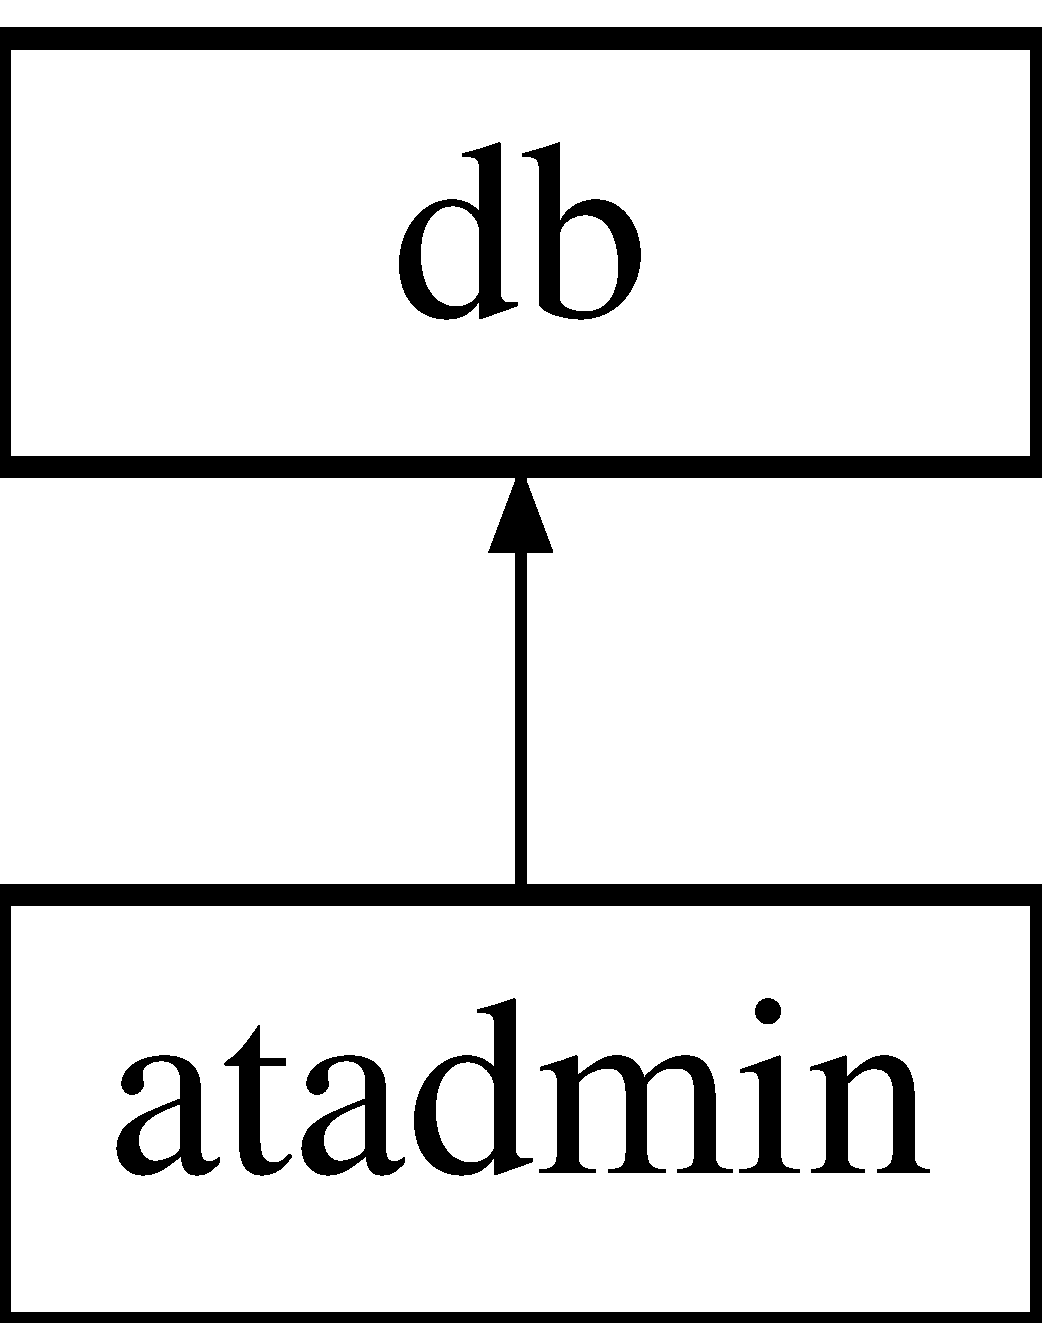
\includegraphics[height=2.000000cm]{classatadmin}
\end{center}
\end{figure}
\subsection*{Public Member Functions}
\begin{DoxyCompactItemize}
\item 
\hyperlink{classatadmin_a7b79f8f3cfeb01295b1910b47f177d68}{create\-Class} (\$Mod\-I\-D, \$class\-Start, \$class\-End, \$qr\-M\-D5)
\item 
\hyperlink{classatadmin_ace33597a2778eceac70fc2dbab17ef74}{get\-Class\-I\-D} (\$qr\-M\-D5)
\end{DoxyCompactItemize}
\subsection*{Additional Inherited Members}


\subsection{Member Function Documentation}
\hypertarget{classatadmin_a7b79f8f3cfeb01295b1910b47f177d68}{\index{atadmin@{atadmin}!create\-Class@{create\-Class}}
\index{create\-Class@{create\-Class}!atadmin@{atadmin}}
\subsubsection[{create\-Class}]{\setlength{\rightskip}{0pt plus 5cm}create\-Class (
\begin{DoxyParamCaption}
\item[{}]{\$\-Mod\-I\-D, }
\item[{}]{\$class\-Start, }
\item[{}]{\$class\-End, }
\item[{}]{\$qr\-M\-D5}
\end{DoxyParamCaption}
)}}\label{classatadmin_a7b79f8f3cfeb01295b1910b47f177d68}
\hypertarget{classatadmin_ace33597a2778eceac70fc2dbab17ef74}{\index{atadmin@{atadmin}!get\-Class\-I\-D@{get\-Class\-I\-D}}
\index{get\-Class\-I\-D@{get\-Class\-I\-D}!atadmin@{atadmin}}
\subsubsection[{get\-Class\-I\-D}]{\setlength{\rightskip}{0pt plus 5cm}get\-Class\-I\-D (
\begin{DoxyParamCaption}
\item[{}]{\$qr\-M\-D5}
\end{DoxyParamCaption}
)}}\label{classatadmin_ace33597a2778eceac70fc2dbab17ef74}


The documentation for this class was generated from the following file\-:\begin{DoxyCompactItemize}
\item 
C\-:/wamp/www/vesey.\-atspace.\-eu/db/\hyperlink{atadmin_8php}{atadmin.\-php}\end{DoxyCompactItemize}

\hypertarget{classdb}{\section{db Class Reference}
\label{classdb}\index{db@{db}}
}
Inheritance diagram for db\-:\begin{figure}[H]
\begin{center}
\leavevmode
\includegraphics[height=2.000000cm]{classdb}
\end{center}
\end{figure}
\subsection*{Public Member Functions}
\begin{DoxyCompactItemize}
\item 
\hyperlink{classdb_aadb6cdfdaf2a6596ecbe1a60e24b51ac}{condb} ()
\item 
\hyperlink{classdb_aa36d52ba4bb4a7696119c537187a37eb}{closedb} ()
\item 
\hyperlink{classdb_a95ff0a9a55f03aaade9edbb977595061}{checklogin} ()
\item 
\hyperlink{classdb_ad870c94a5775868891f6c50b9818d627}{login} (\$username, \$password)
\item 
\hyperlink{classdb_ae8aa276bf5607f9dc5e8877d18cec9a5}{log\-Attend} (\$class, \$username, \$password)
\item 
\hyperlink{classdb_a81b37a3c9d639574e394f80c1138c75e}{get\-Username} ()
\item 
\hyperlink{classdb_a04e0957baeb7acde9c0c86556da2d43f}{get\-Password} ()
\item 
\hyperlink{classdb_aab5647a5bd77aa3eb60010b4258ae11e}{get\-Courses} (\$User\-I\-D)
\item 
\hyperlink{classdb_aafaff27dbe8ed98b9ce03af5047b2d22}{get\-Mod\-Attend} (\$module)
\item 
\hyperlink{classdb_ac87d4cfaf79b234def1019bd9faa9421}{format\-X\-M\-L} (\$result, \$root\-Element\-Name, \$child\-Element\-Name)
\item 
\hyperlink{classdb_a6413de1c7e932e73b97142084a9e4a40}{get\-Mod\-Access\-Level} (\$module)
\item 
\hyperlink{classdb_a723148b84aa331ce72baf09cdaedcabe}{get\-Overall\-Attend} (\$module)
\end{DoxyCompactItemize}
\subsection*{Protected Attributes}
\begin{DoxyCompactItemize}
\item 
\hyperlink{classdb_a82912d256f27bdb90a9114b053eb07c8}{\$\-\_\-dcon} = \char`\"{}\char`\"{}
\end{DoxyCompactItemize}


\subsection{Member Function Documentation}
\hypertarget{classdb_a95ff0a9a55f03aaade9edbb977595061}{\index{db@{db}!checklogin@{checklogin}}
\index{checklogin@{checklogin}!db@{db}}
\subsubsection[{checklogin}]{\setlength{\rightskip}{0pt plus 5cm}checklogin (
\begin{DoxyParamCaption}
{}
\end{DoxyParamCaption}
)}}\label{classdb_a95ff0a9a55f03aaade9edbb977595061}
\hypertarget{classdb_aa36d52ba4bb4a7696119c537187a37eb}{\index{db@{db}!closedb@{closedb}}
\index{closedb@{closedb}!db@{db}}
\subsubsection[{closedb}]{\setlength{\rightskip}{0pt plus 5cm}closedb (
\begin{DoxyParamCaption}
{}
\end{DoxyParamCaption}
)}}\label{classdb_aa36d52ba4bb4a7696119c537187a37eb}
\hypertarget{classdb_aadb6cdfdaf2a6596ecbe1a60e24b51ac}{\index{db@{db}!condb@{condb}}
\index{condb@{condb}!db@{db}}
\subsubsection[{condb}]{\setlength{\rightskip}{0pt plus 5cm}condb (
\begin{DoxyParamCaption}
{}
\end{DoxyParamCaption}
)}}\label{classdb_aadb6cdfdaf2a6596ecbe1a60e24b51ac}
\hypertarget{classdb_ac87d4cfaf79b234def1019bd9faa9421}{\index{db@{db}!format\-X\-M\-L@{format\-X\-M\-L}}
\index{format\-X\-M\-L@{format\-X\-M\-L}!db@{db}}
\subsubsection[{format\-X\-M\-L}]{\setlength{\rightskip}{0pt plus 5cm}format\-X\-M\-L (
\begin{DoxyParamCaption}
\item[{}]{\$result, }
\item[{}]{\$root\-Element\-Name, }
\item[{}]{\$child\-Element\-Name}
\end{DoxyParamCaption}
)}}\label{classdb_ac87d4cfaf79b234def1019bd9faa9421}
\hypertarget{classdb_aab5647a5bd77aa3eb60010b4258ae11e}{\index{db@{db}!get\-Courses@{get\-Courses}}
\index{get\-Courses@{get\-Courses}!db@{db}}
\subsubsection[{get\-Courses}]{\setlength{\rightskip}{0pt plus 5cm}get\-Courses (
\begin{DoxyParamCaption}
\item[{}]{\$\-User\-I\-D}
\end{DoxyParamCaption}
)}}\label{classdb_aab5647a5bd77aa3eb60010b4258ae11e}
\hypertarget{classdb_a6413de1c7e932e73b97142084a9e4a40}{\index{db@{db}!get\-Mod\-Access\-Level@{get\-Mod\-Access\-Level}}
\index{get\-Mod\-Access\-Level@{get\-Mod\-Access\-Level}!db@{db}}
\subsubsection[{get\-Mod\-Access\-Level}]{\setlength{\rightskip}{0pt plus 5cm}get\-Mod\-Access\-Level (
\begin{DoxyParamCaption}
\item[{}]{\$module}
\end{DoxyParamCaption}
)}}\label{classdb_a6413de1c7e932e73b97142084a9e4a40}
\hypertarget{classdb_aafaff27dbe8ed98b9ce03af5047b2d22}{\index{db@{db}!get\-Mod\-Attend@{get\-Mod\-Attend}}
\index{get\-Mod\-Attend@{get\-Mod\-Attend}!db@{db}}
\subsubsection[{get\-Mod\-Attend}]{\setlength{\rightskip}{0pt plus 5cm}get\-Mod\-Attend (
\begin{DoxyParamCaption}
\item[{}]{\$module}
\end{DoxyParamCaption}
)}}\label{classdb_aafaff27dbe8ed98b9ce03af5047b2d22}
\hypertarget{classdb_a723148b84aa331ce72baf09cdaedcabe}{\index{db@{db}!get\-Overall\-Attend@{get\-Overall\-Attend}}
\index{get\-Overall\-Attend@{get\-Overall\-Attend}!db@{db}}
\subsubsection[{get\-Overall\-Attend}]{\setlength{\rightskip}{0pt plus 5cm}get\-Overall\-Attend (
\begin{DoxyParamCaption}
\item[{}]{\$module}
\end{DoxyParamCaption}
)}}\label{classdb_a723148b84aa331ce72baf09cdaedcabe}
\hypertarget{classdb_a04e0957baeb7acde9c0c86556da2d43f}{\index{db@{db}!get\-Password@{get\-Password}}
\index{get\-Password@{get\-Password}!db@{db}}
\subsubsection[{get\-Password}]{\setlength{\rightskip}{0pt plus 5cm}get\-Password (
\begin{DoxyParamCaption}
{}
\end{DoxyParamCaption}
)}}\label{classdb_a04e0957baeb7acde9c0c86556da2d43f}
\hypertarget{classdb_a81b37a3c9d639574e394f80c1138c75e}{\index{db@{db}!get\-Username@{get\-Username}}
\index{get\-Username@{get\-Username}!db@{db}}
\subsubsection[{get\-Username}]{\setlength{\rightskip}{0pt plus 5cm}get\-Username (
\begin{DoxyParamCaption}
{}
\end{DoxyParamCaption}
)}}\label{classdb_a81b37a3c9d639574e394f80c1138c75e}
\hypertarget{classdb_ae8aa276bf5607f9dc5e8877d18cec9a5}{\index{db@{db}!log\-Attend@{log\-Attend}}
\index{log\-Attend@{log\-Attend}!db@{db}}
\subsubsection[{log\-Attend}]{\setlength{\rightskip}{0pt plus 5cm}log\-Attend (
\begin{DoxyParamCaption}
\item[{}]{\$class, }
\item[{}]{\$username, }
\item[{}]{\$password}
\end{DoxyParamCaption}
)}}\label{classdb_ae8aa276bf5607f9dc5e8877d18cec9a5}
\hypertarget{classdb_ad870c94a5775868891f6c50b9818d627}{\index{db@{db}!login@{login}}
\index{login@{login}!db@{db}}
\subsubsection[{login}]{\setlength{\rightskip}{0pt plus 5cm}login (
\begin{DoxyParamCaption}
\item[{}]{\$username, }
\item[{}]{\$password}
\end{DoxyParamCaption}
)}}\label{classdb_ad870c94a5775868891f6c50b9818d627}


\subsection{Field Documentation}
\hypertarget{classdb_a82912d256f27bdb90a9114b053eb07c8}{\index{db@{db}!\$\-\_\-dcon@{\$\-\_\-dcon}}
\index{\$\-\_\-dcon@{\$\-\_\-dcon}!db@{db}}
\subsubsection[{\$\-\_\-dcon}]{\setlength{\rightskip}{0pt plus 5cm}\$\-\_\-dcon = \char`\"{}\char`\"{}\hspace{0.3cm}{\ttfamily [protected]}}}\label{classdb_a82912d256f27bdb90a9114b053eb07c8}


The documentation for this class was generated from the following file\-:\begin{DoxyCompactItemize}
\item 
C\-:/wamp/www/vesey.\-atspace.\-eu/db/\hyperlink{db_8php}{db.\-php}\end{DoxyCompactItemize}

\hypertarget{class_frame_filler}{\section{Frame\-Filler Class Reference}
\label{class_frame_filler}\index{Frame\-Filler@{Frame\-Filler}}
}
\subsection*{Public Member Functions}
\begin{DoxyCompactItemize}
\item 
\hyperlink{class_frame_filler_a4257c01489a1295e5907060176af470b}{\-\_\-\-\_\-construct} (\$width, \&\$frame)
\item 
\hyperlink{class_frame_filler_a116b16f8a805109f74df9c28355282ce}{set\-Frame\-At} (\$at, \$val)
\item 
\hyperlink{class_frame_filler_a29a104e9c06167abd578b41e38217b09}{get\-Frame\-At} (\$at)
\item 
\hyperlink{class_frame_filler_acea62048bfee7b3cd80ed446c86fb78a}{next} ()
\end{DoxyCompactItemize}
\subsection*{Data Fields}
\begin{DoxyCompactItemize}
\item 
\hyperlink{class_frame_filler_a5795120b4b324bc4ca83f1e6fdce7d57}{\$width}
\item 
\hyperlink{class_frame_filler_a2c5e909bcaf7c8dfc4672361f47867ee}{\$frame}
\item 
\hyperlink{class_frame_filler_af3a16c5f0dd7a74cf9acf6a49fff73a7}{\$x}
\item 
\hyperlink{class_frame_filler_a77b973d137fb33212e018b042df6e3e7}{\$y}
\item 
\hyperlink{class_frame_filler_a1659f0a629d408e0f849dbe4ee061e62}{\$dir}
\item 
\hyperlink{class_frame_filler_a43ea1718834af94a8cbebd17611666ae}{\$bit}
\end{DoxyCompactItemize}


\subsection{Constructor \& Destructor Documentation}
\hypertarget{class_frame_filler_a4257c01489a1295e5907060176af470b}{\index{Frame\-Filler@{Frame\-Filler}!\-\_\-\-\_\-construct@{\-\_\-\-\_\-construct}}
\index{\-\_\-\-\_\-construct@{\-\_\-\-\_\-construct}!FrameFiller@{Frame\-Filler}}
\subsubsection[{\-\_\-\-\_\-construct}]{\setlength{\rightskip}{0pt plus 5cm}\-\_\-\-\_\-construct (
\begin{DoxyParamCaption}
\item[{}]{\$width, }
\item[{\&}]{\$frame}
\end{DoxyParamCaption}
)}}\label{class_frame_filler_a4257c01489a1295e5907060176af470b}


\subsection{Member Function Documentation}
\hypertarget{class_frame_filler_a29a104e9c06167abd578b41e38217b09}{\index{Frame\-Filler@{Frame\-Filler}!get\-Frame\-At@{get\-Frame\-At}}
\index{get\-Frame\-At@{get\-Frame\-At}!FrameFiller@{Frame\-Filler}}
\subsubsection[{get\-Frame\-At}]{\setlength{\rightskip}{0pt plus 5cm}get\-Frame\-At (
\begin{DoxyParamCaption}
\item[{}]{\$at}
\end{DoxyParamCaption}
)}}\label{class_frame_filler_a29a104e9c06167abd578b41e38217b09}
\hypertarget{class_frame_filler_acea62048bfee7b3cd80ed446c86fb78a}{\index{Frame\-Filler@{Frame\-Filler}!next@{next}}
\index{next@{next}!FrameFiller@{Frame\-Filler}}
\subsubsection[{next}]{\setlength{\rightskip}{0pt plus 5cm}next (
\begin{DoxyParamCaption}
{}
\end{DoxyParamCaption}
)}}\label{class_frame_filler_acea62048bfee7b3cd80ed446c86fb78a}
\hypertarget{class_frame_filler_a116b16f8a805109f74df9c28355282ce}{\index{Frame\-Filler@{Frame\-Filler}!set\-Frame\-At@{set\-Frame\-At}}
\index{set\-Frame\-At@{set\-Frame\-At}!FrameFiller@{Frame\-Filler}}
\subsubsection[{set\-Frame\-At}]{\setlength{\rightskip}{0pt plus 5cm}set\-Frame\-At (
\begin{DoxyParamCaption}
\item[{}]{\$at, }
\item[{}]{\$val}
\end{DoxyParamCaption}
)}}\label{class_frame_filler_a116b16f8a805109f74df9c28355282ce}


\subsection{Field Documentation}
\hypertarget{class_frame_filler_a43ea1718834af94a8cbebd17611666ae}{\index{Frame\-Filler@{Frame\-Filler}!\$bit@{\$bit}}
\index{\$bit@{\$bit}!FrameFiller@{Frame\-Filler}}
\subsubsection[{\$bit}]{\setlength{\rightskip}{0pt plus 5cm}\$bit}}\label{class_frame_filler_a43ea1718834af94a8cbebd17611666ae}
\hypertarget{class_frame_filler_a1659f0a629d408e0f849dbe4ee061e62}{\index{Frame\-Filler@{Frame\-Filler}!\$dir@{\$dir}}
\index{\$dir@{\$dir}!FrameFiller@{Frame\-Filler}}
\subsubsection[{\$dir}]{\setlength{\rightskip}{0pt plus 5cm}\$dir}}\label{class_frame_filler_a1659f0a629d408e0f849dbe4ee061e62}
\hypertarget{class_frame_filler_a2c5e909bcaf7c8dfc4672361f47867ee}{\index{Frame\-Filler@{Frame\-Filler}!\$frame@{\$frame}}
\index{\$frame@{\$frame}!FrameFiller@{Frame\-Filler}}
\subsubsection[{\$frame}]{\setlength{\rightskip}{0pt plus 5cm}\$frame}}\label{class_frame_filler_a2c5e909bcaf7c8dfc4672361f47867ee}
\hypertarget{class_frame_filler_a5795120b4b324bc4ca83f1e6fdce7d57}{\index{Frame\-Filler@{Frame\-Filler}!\$width@{\$width}}
\index{\$width@{\$width}!FrameFiller@{Frame\-Filler}}
\subsubsection[{\$width}]{\setlength{\rightskip}{0pt plus 5cm}\$width}}\label{class_frame_filler_a5795120b4b324bc4ca83f1e6fdce7d57}
\hypertarget{class_frame_filler_af3a16c5f0dd7a74cf9acf6a49fff73a7}{\index{Frame\-Filler@{Frame\-Filler}!\$x@{\$x}}
\index{\$x@{\$x}!FrameFiller@{Frame\-Filler}}
\subsubsection[{\$x}]{\setlength{\rightskip}{0pt plus 5cm}\$x}}\label{class_frame_filler_af3a16c5f0dd7a74cf9acf6a49fff73a7}
\hypertarget{class_frame_filler_a77b973d137fb33212e018b042df6e3e7}{\index{Frame\-Filler@{Frame\-Filler}!\$y@{\$y}}
\index{\$y@{\$y}!FrameFiller@{Frame\-Filler}}
\subsubsection[{\$y}]{\setlength{\rightskip}{0pt plus 5cm}\$y}}\label{class_frame_filler_a77b973d137fb33212e018b042df6e3e7}


The documentation for this class was generated from the following file\-:\begin{DoxyCompactItemize}
\item 
C\-:/wamp/www/vesey.\-atspace.\-eu/qr/\hyperlink{qrencode_8php}{qrencode.\-php}\end{DoxyCompactItemize}

\hypertarget{classqr}{\section{qr Class Reference}
\label{classqr}\index{qr@{qr}}
}
\subsection*{Public Member Functions}
\begin{DoxyCompactItemize}
\item 
\hyperlink{classqr_add85d8c27a6bd7d4c55066800dbcb078}{distroyqr} ()
\item 
\hyperlink{classqr_af360cd17cda1feaa24049df204c71a07}{make\-Q\-R\-Code} (\$md5)
\end{DoxyCompactItemize}


\subsection{Member Function Documentation}
\hypertarget{classqr_add85d8c27a6bd7d4c55066800dbcb078}{\index{qr@{qr}!distroyqr@{distroyqr}}
\index{distroyqr@{distroyqr}!qr@{qr}}
\subsubsection[{distroyqr}]{\setlength{\rightskip}{0pt plus 5cm}distroyqr (
\begin{DoxyParamCaption}
{}
\end{DoxyParamCaption}
)}}\label{classqr_add85d8c27a6bd7d4c55066800dbcb078}
\hypertarget{classqr_af360cd17cda1feaa24049df204c71a07}{\index{qr@{qr}!make\-Q\-R\-Code@{make\-Q\-R\-Code}}
\index{make\-Q\-R\-Code@{make\-Q\-R\-Code}!qr@{qr}}
\subsubsection[{make\-Q\-R\-Code}]{\setlength{\rightskip}{0pt plus 5cm}make\-Q\-R\-Code (
\begin{DoxyParamCaption}
\item[{}]{\$md5}
\end{DoxyParamCaption}
)}}\label{classqr_af360cd17cda1feaa24049df204c71a07}


The documentation for this class was generated from the following file\-:\begin{DoxyCompactItemize}
\item 
C\-:/wamp/www/vesey.\-atspace.\-eu/qr/\hyperlink{qr_8php}{qr.\-php}\end{DoxyCompactItemize}

\hypertarget{class_q_rbitstream}{\section{Q\-Rbitstream Class Reference}
\label{class_q_rbitstream}\index{Q\-Rbitstream@{Q\-Rbitstream}}
}
\subsection*{Public Member Functions}
\begin{DoxyCompactItemize}
\item 
\hyperlink{class_q_rbitstream_a775bfb88c1bb7975d67f277eade2a1b7}{size} ()
\item 
\hyperlink{class_q_rbitstream_adc9952419d09d0d0afedfacd4471433f}{allocate} (\$set\-Length)
\item 
\hyperlink{class_q_rbitstream_a75000673a2a1620408fbf91ccc31e7b0}{append} (\hyperlink{class_q_rbitstream}{Q\-Rbitstream} \$arg)
\item 
\hyperlink{class_q_rbitstream_a99b3b6b2a865deb3d1945aebd07c3bf3}{append\-Num} (\$bits, \$num)
\item 
\hyperlink{class_q_rbitstream_acca7cd6db4b1ff6eddf243ccb3d90b9b}{append\-Bytes} (\$\hyperlink{class_q_rbitstream_a775bfb88c1bb7975d67f277eade2a1b7}{size}, \$data)
\item 
\hyperlink{class_q_rbitstream_a084c4c03b3b0c907ce584eac4eecd475}{to\-Byte} ()
\end{DoxyCompactItemize}
\subsection*{Static Public Member Functions}
\begin{DoxyCompactItemize}
\item 
static \hyperlink{class_q_rbitstream_a7d553d41faeb9fed6099a106f9ad64da}{new\-From\-Num} (\$bits, \$num)
\item 
static \hyperlink{class_q_rbitstream_a233d5da4c0c11b8dbda14d10349e55e2}{new\-From\-Bytes} (\$\hyperlink{class_q_rbitstream_a775bfb88c1bb7975d67f277eade2a1b7}{size}, \$data)
\end{DoxyCompactItemize}
\subsection*{Data Fields}
\begin{DoxyCompactItemize}
\item 
\hyperlink{class_q_rbitstream_a6efc15b5a2314dd4b5aaa556a375c6d6}{\$data} = array()
\end{DoxyCompactItemize}


\subsection{Member Function Documentation}
\hypertarget{class_q_rbitstream_adc9952419d09d0d0afedfacd4471433f}{\index{Q\-Rbitstream@{Q\-Rbitstream}!allocate@{allocate}}
\index{allocate@{allocate}!QRbitstream@{Q\-Rbitstream}}
\subsubsection[{allocate}]{\setlength{\rightskip}{0pt plus 5cm}allocate (
\begin{DoxyParamCaption}
\item[{}]{\$set\-Length}
\end{DoxyParamCaption}
)}}\label{class_q_rbitstream_adc9952419d09d0d0afedfacd4471433f}
\hypertarget{class_q_rbitstream_a75000673a2a1620408fbf91ccc31e7b0}{\index{Q\-Rbitstream@{Q\-Rbitstream}!append@{append}}
\index{append@{append}!QRbitstream@{Q\-Rbitstream}}
\subsubsection[{append}]{\setlength{\rightskip}{0pt plus 5cm}append (
\begin{DoxyParamCaption}
\item[{{\bf Q\-Rbitstream}}]{\$arg}
\end{DoxyParamCaption}
)}}\label{class_q_rbitstream_a75000673a2a1620408fbf91ccc31e7b0}
\hypertarget{class_q_rbitstream_acca7cd6db4b1ff6eddf243ccb3d90b9b}{\index{Q\-Rbitstream@{Q\-Rbitstream}!append\-Bytes@{append\-Bytes}}
\index{append\-Bytes@{append\-Bytes}!QRbitstream@{Q\-Rbitstream}}
\subsubsection[{append\-Bytes}]{\setlength{\rightskip}{0pt plus 5cm}append\-Bytes (
\begin{DoxyParamCaption}
\item[{}]{\$size, }
\item[{}]{\$data}
\end{DoxyParamCaption}
)}}\label{class_q_rbitstream_acca7cd6db4b1ff6eddf243ccb3d90b9b}
\hypertarget{class_q_rbitstream_a99b3b6b2a865deb3d1945aebd07c3bf3}{\index{Q\-Rbitstream@{Q\-Rbitstream}!append\-Num@{append\-Num}}
\index{append\-Num@{append\-Num}!QRbitstream@{Q\-Rbitstream}}
\subsubsection[{append\-Num}]{\setlength{\rightskip}{0pt plus 5cm}append\-Num (
\begin{DoxyParamCaption}
\item[{}]{\$bits, }
\item[{}]{\$num}
\end{DoxyParamCaption}
)}}\label{class_q_rbitstream_a99b3b6b2a865deb3d1945aebd07c3bf3}
\hypertarget{class_q_rbitstream_a233d5da4c0c11b8dbda14d10349e55e2}{\index{Q\-Rbitstream@{Q\-Rbitstream}!new\-From\-Bytes@{new\-From\-Bytes}}
\index{new\-From\-Bytes@{new\-From\-Bytes}!QRbitstream@{Q\-Rbitstream}}
\subsubsection[{new\-From\-Bytes}]{\setlength{\rightskip}{0pt plus 5cm}static new\-From\-Bytes (
\begin{DoxyParamCaption}
\item[{}]{\$size, }
\item[{}]{\$data}
\end{DoxyParamCaption}
)\hspace{0.3cm}{\ttfamily [static]}}}\label{class_q_rbitstream_a233d5da4c0c11b8dbda14d10349e55e2}
\hypertarget{class_q_rbitstream_a7d553d41faeb9fed6099a106f9ad64da}{\index{Q\-Rbitstream@{Q\-Rbitstream}!new\-From\-Num@{new\-From\-Num}}
\index{new\-From\-Num@{new\-From\-Num}!QRbitstream@{Q\-Rbitstream}}
\subsubsection[{new\-From\-Num}]{\setlength{\rightskip}{0pt plus 5cm}static new\-From\-Num (
\begin{DoxyParamCaption}
\item[{}]{\$bits, }
\item[{}]{\$num}
\end{DoxyParamCaption}
)\hspace{0.3cm}{\ttfamily [static]}}}\label{class_q_rbitstream_a7d553d41faeb9fed6099a106f9ad64da}
\hypertarget{class_q_rbitstream_a775bfb88c1bb7975d67f277eade2a1b7}{\index{Q\-Rbitstream@{Q\-Rbitstream}!size@{size}}
\index{size@{size}!QRbitstream@{Q\-Rbitstream}}
\subsubsection[{size}]{\setlength{\rightskip}{0pt plus 5cm}size (
\begin{DoxyParamCaption}
{}
\end{DoxyParamCaption}
)}}\label{class_q_rbitstream_a775bfb88c1bb7975d67f277eade2a1b7}
\hypertarget{class_q_rbitstream_a084c4c03b3b0c907ce584eac4eecd475}{\index{Q\-Rbitstream@{Q\-Rbitstream}!to\-Byte@{to\-Byte}}
\index{to\-Byte@{to\-Byte}!QRbitstream@{Q\-Rbitstream}}
\subsubsection[{to\-Byte}]{\setlength{\rightskip}{0pt plus 5cm}to\-Byte (
\begin{DoxyParamCaption}
{}
\end{DoxyParamCaption}
)}}\label{class_q_rbitstream_a084c4c03b3b0c907ce584eac4eecd475}


\subsection{Field Documentation}
\hypertarget{class_q_rbitstream_a6efc15b5a2314dd4b5aaa556a375c6d6}{\index{Q\-Rbitstream@{Q\-Rbitstream}!\$data@{\$data}}
\index{\$data@{\$data}!QRbitstream@{Q\-Rbitstream}}
\subsubsection[{\$data}]{\setlength{\rightskip}{0pt plus 5cm}\$data = array()}}\label{class_q_rbitstream_a6efc15b5a2314dd4b5aaa556a375c6d6}


The documentation for this class was generated from the following file\-:\begin{DoxyCompactItemize}
\item 
C\-:/wamp/www/vesey.\-atspace.\-eu/qr/\hyperlink{qrbitstream_8php}{qrbitstream.\-php}\end{DoxyCompactItemize}

\hypertarget{class_q_rcode}{\section{Q\-Rcode Class Reference}
\label{class_q_rcode}\index{Q\-Rcode@{Q\-Rcode}}
}
\subsection*{Public Member Functions}
\begin{DoxyCompactItemize}
\item 
\hyperlink{class_q_rcode_acf42d0cdad5d76be2def212ac6b97d96}{encode\-Mask} (\hyperlink{class_q_rinput}{Q\-Rinput} \$input, \$mask)
\item 
\hyperlink{class_q_rcode_ab5a5a1beab6c2d2e456fe81c7d2c91fd}{encode\-Input} (\hyperlink{class_q_rinput}{Q\-Rinput} \$input)
\item 
\hyperlink{class_q_rcode_ae2c56d379dde08a538d0e8ea41a40249}{encode\-String8bit} (\$string, \$version, \$level)
\item 
\hyperlink{class_q_rcode_ae7268450e652c25d1bdb58f915fe6aee}{encode\-String} (\$string, \$version, \$level, \$hint, \$casesensitive)
\end{DoxyCompactItemize}
\subsection*{Static Public Member Functions}
\begin{DoxyCompactItemize}
\item 
static \hyperlink{class_q_rcode_af1ddbe08ddc863554785e57c0a6b5162}{png} (\$\hyperlink{class_q_rcode_a6d3a6d648171f75856c70d5b7e727d51}{text}, \$outfile=false, \$level=\hyperlink{qrconst_8php_ae106d3baebd9c27c90b2abadb25df012}{Q\-R\-\_\-\-E\-C\-L\-E\-V\-E\-L\-\_\-\-L}, \$size=3, \$margin=4, \$saveandprint=false)
\item 
static \hyperlink{class_q_rcode_a6d3a6d648171f75856c70d5b7e727d51}{text} (\$text, \$outfile=false, \$level=\hyperlink{qrconst_8php_ae106d3baebd9c27c90b2abadb25df012}{Q\-R\-\_\-\-E\-C\-L\-E\-V\-E\-L\-\_\-\-L}, \$size=3, \$margin=4)
\item 
static \hyperlink{class_q_rcode_a87ffd66d8e405c5c98d5e0f3c7a5f914}{raw} (\$\hyperlink{class_q_rcode_a6d3a6d648171f75856c70d5b7e727d51}{text}, \$outfile=false, \$level=\hyperlink{qrconst_8php_ae106d3baebd9c27c90b2abadb25df012}{Q\-R\-\_\-\-E\-C\-L\-E\-V\-E\-L\-\_\-\-L}, \$size=3, \$margin=4)
\end{DoxyCompactItemize}
\subsection*{Data Fields}
\begin{DoxyCompactItemize}
\item 
\hyperlink{class_q_rcode_a17c8948c68aa44fa9961ae169b6a8961}{\$version}
\item 
\hyperlink{class_q_rcode_a5795120b4b324bc4ca83f1e6fdce7d57}{\$width}
\item 
\hyperlink{class_q_rcode_a6efc15b5a2314dd4b5aaa556a375c6d6}{\$data}
\end{DoxyCompactItemize}


\subsection{Member Function Documentation}
\hypertarget{class_q_rcode_ab5a5a1beab6c2d2e456fe81c7d2c91fd}{\index{Q\-Rcode@{Q\-Rcode}!encode\-Input@{encode\-Input}}
\index{encode\-Input@{encode\-Input}!QRcode@{Q\-Rcode}}
\subsubsection[{encode\-Input}]{\setlength{\rightskip}{0pt plus 5cm}encode\-Input (
\begin{DoxyParamCaption}
\item[{{\bf Q\-Rinput}}]{\$input}
\end{DoxyParamCaption}
)}}\label{class_q_rcode_ab5a5a1beab6c2d2e456fe81c7d2c91fd}
\hypertarget{class_q_rcode_acf42d0cdad5d76be2def212ac6b97d96}{\index{Q\-Rcode@{Q\-Rcode}!encode\-Mask@{encode\-Mask}}
\index{encode\-Mask@{encode\-Mask}!QRcode@{Q\-Rcode}}
\subsubsection[{encode\-Mask}]{\setlength{\rightskip}{0pt plus 5cm}encode\-Mask (
\begin{DoxyParamCaption}
\item[{{\bf Q\-Rinput}}]{\$input, }
\item[{}]{\$mask}
\end{DoxyParamCaption}
)}}\label{class_q_rcode_acf42d0cdad5d76be2def212ac6b97d96}
\hypertarget{class_q_rcode_ae7268450e652c25d1bdb58f915fe6aee}{\index{Q\-Rcode@{Q\-Rcode}!encode\-String@{encode\-String}}
\index{encode\-String@{encode\-String}!QRcode@{Q\-Rcode}}
\subsubsection[{encode\-String}]{\setlength{\rightskip}{0pt plus 5cm}encode\-String (
\begin{DoxyParamCaption}
\item[{}]{\$string, }
\item[{}]{\$version, }
\item[{}]{\$level, }
\item[{}]{\$hint, }
\item[{}]{\$casesensitive}
\end{DoxyParamCaption}
)}}\label{class_q_rcode_ae7268450e652c25d1bdb58f915fe6aee}
\hypertarget{class_q_rcode_ae2c56d379dde08a538d0e8ea41a40249}{\index{Q\-Rcode@{Q\-Rcode}!encode\-String8bit@{encode\-String8bit}}
\index{encode\-String8bit@{encode\-String8bit}!QRcode@{Q\-Rcode}}
\subsubsection[{encode\-String8bit}]{\setlength{\rightskip}{0pt plus 5cm}encode\-String8bit (
\begin{DoxyParamCaption}
\item[{}]{\$string, }
\item[{}]{\$version, }
\item[{}]{\$level}
\end{DoxyParamCaption}
)}}\label{class_q_rcode_ae2c56d379dde08a538d0e8ea41a40249}
\hypertarget{class_q_rcode_af1ddbe08ddc863554785e57c0a6b5162}{\index{Q\-Rcode@{Q\-Rcode}!png@{png}}
\index{png@{png}!QRcode@{Q\-Rcode}}
\subsubsection[{png}]{\setlength{\rightskip}{0pt plus 5cm}static png (
\begin{DoxyParamCaption}
\item[{}]{\$text, }
\item[{}]{\$outfile = {\ttfamily false}, }
\item[{}]{\$level = {\ttfamily {\bf Q\-R\-\_\-\-E\-C\-L\-E\-V\-E\-L\-\_\-\-L}}, }
\item[{}]{\$size = {\ttfamily 3}, }
\item[{}]{\$margin = {\ttfamily 4}, }
\item[{}]{\$saveandprint = {\ttfamily false}}
\end{DoxyParamCaption}
)\hspace{0.3cm}{\ttfamily [static]}}}\label{class_q_rcode_af1ddbe08ddc863554785e57c0a6b5162}
\hypertarget{class_q_rcode_a87ffd66d8e405c5c98d5e0f3c7a5f914}{\index{Q\-Rcode@{Q\-Rcode}!raw@{raw}}
\index{raw@{raw}!QRcode@{Q\-Rcode}}
\subsubsection[{raw}]{\setlength{\rightskip}{0pt plus 5cm}static raw (
\begin{DoxyParamCaption}
\item[{}]{\$text, }
\item[{}]{\$outfile = {\ttfamily false}, }
\item[{}]{\$level = {\ttfamily {\bf Q\-R\-\_\-\-E\-C\-L\-E\-V\-E\-L\-\_\-\-L}}, }
\item[{}]{\$size = {\ttfamily 3}, }
\item[{}]{\$margin = {\ttfamily 4}}
\end{DoxyParamCaption}
)\hspace{0.3cm}{\ttfamily [static]}}}\label{class_q_rcode_a87ffd66d8e405c5c98d5e0f3c7a5f914}
\hypertarget{class_q_rcode_a6d3a6d648171f75856c70d5b7e727d51}{\index{Q\-Rcode@{Q\-Rcode}!text@{text}}
\index{text@{text}!QRcode@{Q\-Rcode}}
\subsubsection[{text}]{\setlength{\rightskip}{0pt plus 5cm}static text (
\begin{DoxyParamCaption}
\item[{}]{\$text, }
\item[{}]{\$outfile = {\ttfamily false}, }
\item[{}]{\$level = {\ttfamily {\bf Q\-R\-\_\-\-E\-C\-L\-E\-V\-E\-L\-\_\-\-L}}, }
\item[{}]{\$size = {\ttfamily 3}, }
\item[{}]{\$margin = {\ttfamily 4}}
\end{DoxyParamCaption}
)\hspace{0.3cm}{\ttfamily [static]}}}\label{class_q_rcode_a6d3a6d648171f75856c70d5b7e727d51}


\subsection{Field Documentation}
\hypertarget{class_q_rcode_a6efc15b5a2314dd4b5aaa556a375c6d6}{\index{Q\-Rcode@{Q\-Rcode}!\$data@{\$data}}
\index{\$data@{\$data}!QRcode@{Q\-Rcode}}
\subsubsection[{\$data}]{\setlength{\rightskip}{0pt plus 5cm}\$data}}\label{class_q_rcode_a6efc15b5a2314dd4b5aaa556a375c6d6}
\hypertarget{class_q_rcode_a17c8948c68aa44fa9961ae169b6a8961}{\index{Q\-Rcode@{Q\-Rcode}!\$version@{\$version}}
\index{\$version@{\$version}!QRcode@{Q\-Rcode}}
\subsubsection[{\$version}]{\setlength{\rightskip}{0pt plus 5cm}\$version}}\label{class_q_rcode_a17c8948c68aa44fa9961ae169b6a8961}
\hypertarget{class_q_rcode_a5795120b4b324bc4ca83f1e6fdce7d57}{\index{Q\-Rcode@{Q\-Rcode}!\$width@{\$width}}
\index{\$width@{\$width}!QRcode@{Q\-Rcode}}
\subsubsection[{\$width}]{\setlength{\rightskip}{0pt plus 5cm}\$width}}\label{class_q_rcode_a5795120b4b324bc4ca83f1e6fdce7d57}


The documentation for this class was generated from the following file\-:\begin{DoxyCompactItemize}
\item 
C\-:/wamp/www/vesey.\-atspace.\-eu/qr/\hyperlink{qrencode_8php}{qrencode.\-php}\end{DoxyCompactItemize}

\hypertarget{class_q_rencode}{\section{Q\-Rencode Class Reference}
\label{class_q_rencode}\index{Q\-Rencode@{Q\-Rencode}}
}
\subsection*{Public Member Functions}
\begin{DoxyCompactItemize}
\item 
\hyperlink{class_q_rencode_af8ed8f99c7502ab956dbaf376fca823d}{encode\-R\-A\-W} (\$intext, \$outfile=false)
\item 
\hyperlink{class_q_rencode_a95064ef9e3bce3de7f067ce50de4b943}{encode} (\$intext, \$outfile=false)
\item 
\hyperlink{class_q_rencode_ac0b9fc2d5171db18552a557afc26d6c8}{encode\-P\-N\-G} (\$intext, \$outfile=false, \$saveandprint=false)
\end{DoxyCompactItemize}
\subsection*{Static Public Member Functions}
\begin{DoxyCompactItemize}
\item 
static \hyperlink{class_q_rencode_a21c0c2ab9b0ac05aec27ba27d576ae24}{factory} (\$level=\hyperlink{qrconst_8php_ae106d3baebd9c27c90b2abadb25df012}{Q\-R\-\_\-\-E\-C\-L\-E\-V\-E\-L\-\_\-\-L}, \$size=3, \$margin=4)
\end{DoxyCompactItemize}
\subsection*{Data Fields}
\begin{DoxyCompactItemize}
\item 
\hyperlink{class_q_rencode_a738d4eedb8dfbe5361ad820cd8fca7c9}{\$casesensitive} = true
\item 
\hyperlink{class_q_rencode_af333d0de58e860998e40201cb1cee3df}{\$eightbit} = false
\item 
\hyperlink{class_q_rencode_a17c8948c68aa44fa9961ae169b6a8961}{\$version} = 0
\item 
\hyperlink{class_q_rencode_af594986e4618a8d6a5d7566617f583c6}{\$size} = 3
\item 
\hyperlink{class_q_rencode_a3bcbb0dc2ef6299e52d39c45188f6bbc}{\$margin} = 4
\item 
\hyperlink{class_q_rencode_ad7eb64c756edb0b0e7973b6967d94ebc}{\$structured} = 0
\item 
\hyperlink{class_q_rencode_abd32cc82c6a3f79491987de36ad580ca}{\$level} = \hyperlink{qrconst_8php_ae106d3baebd9c27c90b2abadb25df012}{Q\-R\-\_\-\-E\-C\-L\-E\-V\-E\-L\-\_\-\-L}
\item 
\hyperlink{class_q_rencode_ac40d3d27b2d848f906775623025116d7}{\$hint} = \hyperlink{qrconst_8php_aa3452182528d53c7b65c6802ad15b772}{Q\-R\-\_\-\-M\-O\-D\-E\-\_\-8}
\end{DoxyCompactItemize}


\subsection{Member Function Documentation}
\hypertarget{class_q_rencode_a95064ef9e3bce3de7f067ce50de4b943}{\index{Q\-Rencode@{Q\-Rencode}!encode@{encode}}
\index{encode@{encode}!QRencode@{Q\-Rencode}}
\subsubsection[{encode}]{\setlength{\rightskip}{0pt plus 5cm}encode (
\begin{DoxyParamCaption}
\item[{}]{\$intext, }
\item[{}]{\$outfile = {\ttfamily false}}
\end{DoxyParamCaption}
)}}\label{class_q_rencode_a95064ef9e3bce3de7f067ce50de4b943}
\hypertarget{class_q_rencode_ac0b9fc2d5171db18552a557afc26d6c8}{\index{Q\-Rencode@{Q\-Rencode}!encode\-P\-N\-G@{encode\-P\-N\-G}}
\index{encode\-P\-N\-G@{encode\-P\-N\-G}!QRencode@{Q\-Rencode}}
\subsubsection[{encode\-P\-N\-G}]{\setlength{\rightskip}{0pt plus 5cm}encode\-P\-N\-G (
\begin{DoxyParamCaption}
\item[{}]{\$intext, }
\item[{}]{\$outfile = {\ttfamily false}, }
\item[{}]{\$saveandprint = {\ttfamily false}}
\end{DoxyParamCaption}
)}}\label{class_q_rencode_ac0b9fc2d5171db18552a557afc26d6c8}
\hypertarget{class_q_rencode_af8ed8f99c7502ab956dbaf376fca823d}{\index{Q\-Rencode@{Q\-Rencode}!encode\-R\-A\-W@{encode\-R\-A\-W}}
\index{encode\-R\-A\-W@{encode\-R\-A\-W}!QRencode@{Q\-Rencode}}
\subsubsection[{encode\-R\-A\-W}]{\setlength{\rightskip}{0pt plus 5cm}encode\-R\-A\-W (
\begin{DoxyParamCaption}
\item[{}]{\$intext, }
\item[{}]{\$outfile = {\ttfamily false}}
\end{DoxyParamCaption}
)}}\label{class_q_rencode_af8ed8f99c7502ab956dbaf376fca823d}
\hypertarget{class_q_rencode_a21c0c2ab9b0ac05aec27ba27d576ae24}{\index{Q\-Rencode@{Q\-Rencode}!factory@{factory}}
\index{factory@{factory}!QRencode@{Q\-Rencode}}
\subsubsection[{factory}]{\setlength{\rightskip}{0pt plus 5cm}static factory (
\begin{DoxyParamCaption}
\item[{}]{\$level = {\ttfamily {\bf Q\-R\-\_\-\-E\-C\-L\-E\-V\-E\-L\-\_\-\-L}}, }
\item[{}]{\$size = {\ttfamily 3}, }
\item[{}]{\$margin = {\ttfamily 4}}
\end{DoxyParamCaption}
)\hspace{0.3cm}{\ttfamily [static]}}}\label{class_q_rencode_a21c0c2ab9b0ac05aec27ba27d576ae24}


\subsection{Field Documentation}
\hypertarget{class_q_rencode_a738d4eedb8dfbe5361ad820cd8fca7c9}{\index{Q\-Rencode@{Q\-Rencode}!\$casesensitive@{\$casesensitive}}
\index{\$casesensitive@{\$casesensitive}!QRencode@{Q\-Rencode}}
\subsubsection[{\$casesensitive}]{\setlength{\rightskip}{0pt plus 5cm}\$casesensitive = true}}\label{class_q_rencode_a738d4eedb8dfbe5361ad820cd8fca7c9}
\hypertarget{class_q_rencode_af333d0de58e860998e40201cb1cee3df}{\index{Q\-Rencode@{Q\-Rencode}!\$eightbit@{\$eightbit}}
\index{\$eightbit@{\$eightbit}!QRencode@{Q\-Rencode}}
\subsubsection[{\$eightbit}]{\setlength{\rightskip}{0pt plus 5cm}\$eightbit = false}}\label{class_q_rencode_af333d0de58e860998e40201cb1cee3df}
\hypertarget{class_q_rencode_ac40d3d27b2d848f906775623025116d7}{\index{Q\-Rencode@{Q\-Rencode}!\$hint@{\$hint}}
\index{\$hint@{\$hint}!QRencode@{Q\-Rencode}}
\subsubsection[{\$hint}]{\setlength{\rightskip}{0pt plus 5cm}\$hint = {\bf Q\-R\-\_\-\-M\-O\-D\-E\-\_\-8}}}\label{class_q_rencode_ac40d3d27b2d848f906775623025116d7}
\hypertarget{class_q_rencode_abd32cc82c6a3f79491987de36ad580ca}{\index{Q\-Rencode@{Q\-Rencode}!\$level@{\$level}}
\index{\$level@{\$level}!QRencode@{Q\-Rencode}}
\subsubsection[{\$level}]{\setlength{\rightskip}{0pt plus 5cm}\$level = {\bf Q\-R\-\_\-\-E\-C\-L\-E\-V\-E\-L\-\_\-\-L}}}\label{class_q_rencode_abd32cc82c6a3f79491987de36ad580ca}
\hypertarget{class_q_rencode_a3bcbb0dc2ef6299e52d39c45188f6bbc}{\index{Q\-Rencode@{Q\-Rencode}!\$margin@{\$margin}}
\index{\$margin@{\$margin}!QRencode@{Q\-Rencode}}
\subsubsection[{\$margin}]{\setlength{\rightskip}{0pt plus 5cm}\$margin = 4}}\label{class_q_rencode_a3bcbb0dc2ef6299e52d39c45188f6bbc}
\hypertarget{class_q_rencode_af594986e4618a8d6a5d7566617f583c6}{\index{Q\-Rencode@{Q\-Rencode}!\$size@{\$size}}
\index{\$size@{\$size}!QRencode@{Q\-Rencode}}
\subsubsection[{\$size}]{\setlength{\rightskip}{0pt plus 5cm}\$size = 3}}\label{class_q_rencode_af594986e4618a8d6a5d7566617f583c6}
\hypertarget{class_q_rencode_ad7eb64c756edb0b0e7973b6967d94ebc}{\index{Q\-Rencode@{Q\-Rencode}!\$structured@{\$structured}}
\index{\$structured@{\$structured}!QRencode@{Q\-Rencode}}
\subsubsection[{\$structured}]{\setlength{\rightskip}{0pt plus 5cm}\$structured = 0}}\label{class_q_rencode_ad7eb64c756edb0b0e7973b6967d94ebc}
\hypertarget{class_q_rencode_a17c8948c68aa44fa9961ae169b6a8961}{\index{Q\-Rencode@{Q\-Rencode}!\$version@{\$version}}
\index{\$version@{\$version}!QRencode@{Q\-Rencode}}
\subsubsection[{\$version}]{\setlength{\rightskip}{0pt plus 5cm}\$version = 0}}\label{class_q_rencode_a17c8948c68aa44fa9961ae169b6a8961}


The documentation for this class was generated from the following file\-:\begin{DoxyCompactItemize}
\item 
C\-:/wamp/www/vesey.\-atspace.\-eu/qr/\hyperlink{qrencode_8php}{qrencode.\-php}\end{DoxyCompactItemize}

\hypertarget{class_q_rimage}{\section{Q\-Rimage Class Reference}
\label{class_q_rimage}\index{Q\-Rimage@{Q\-Rimage}}
}
\subsection*{Static Public Member Functions}
\begin{DoxyCompactItemize}
\item 
static \hyperlink{class_q_rimage_a5cf45ffddabf688340853b091ead49e5}{png} (\$frame, \$filename=false, \$pixel\-Per\-Point=4, \$outer\-Frame=4, \$saveandprint=F\-A\-L\-S\-E)
\item 
static \hyperlink{class_q_rimage_a4d1ddac46a2425f91955db0d7db25ea6}{jpg} (\$frame, \$filename=false, \$pixel\-Per\-Point=8, \$outer\-Frame=4, \$q=85)
\end{DoxyCompactItemize}


\subsection{Member Function Documentation}
\hypertarget{class_q_rimage_a4d1ddac46a2425f91955db0d7db25ea6}{\index{Q\-Rimage@{Q\-Rimage}!jpg@{jpg}}
\index{jpg@{jpg}!QRimage@{Q\-Rimage}}
\subsubsection[{jpg}]{\setlength{\rightskip}{0pt plus 5cm}static jpg (
\begin{DoxyParamCaption}
\item[{}]{\$frame, }
\item[{}]{\$filename = {\ttfamily false}, }
\item[{}]{\$pixel\-Per\-Point = {\ttfamily 8}, }
\item[{}]{\$outer\-Frame = {\ttfamily 4}, }
\item[{}]{\$q = {\ttfamily 85}}
\end{DoxyParamCaption}
)\hspace{0.3cm}{\ttfamily [static]}}}\label{class_q_rimage_a4d1ddac46a2425f91955db0d7db25ea6}
\hypertarget{class_q_rimage_a5cf45ffddabf688340853b091ead49e5}{\index{Q\-Rimage@{Q\-Rimage}!png@{png}}
\index{png@{png}!QRimage@{Q\-Rimage}}
\subsubsection[{png}]{\setlength{\rightskip}{0pt plus 5cm}static png (
\begin{DoxyParamCaption}
\item[{}]{\$frame, }
\item[{}]{\$filename = {\ttfamily false}, }
\item[{}]{\$pixel\-Per\-Point = {\ttfamily 4}, }
\item[{}]{\$outer\-Frame = {\ttfamily 4}, }
\item[{}]{\$saveandprint = {\ttfamily FALSE}}
\end{DoxyParamCaption}
)\hspace{0.3cm}{\ttfamily [static]}}}\label{class_q_rimage_a5cf45ffddabf688340853b091ead49e5}


The documentation for this class was generated from the following file\-:\begin{DoxyCompactItemize}
\item 
C\-:/wamp/www/vesey.\-atspace.\-eu/qr/\hyperlink{qrimage_8php}{qrimage.\-php}\end{DoxyCompactItemize}

\hypertarget{class_q_rinput}{\section{Q\-Rinput Class Reference}
\label{class_q_rinput}\index{Q\-Rinput@{Q\-Rinput}}
}
\subsection*{Public Member Functions}
\begin{DoxyCompactItemize}
\item 
\hyperlink{class_q_rinput_a2351f3e3ad5a02db547f8ee889c3decd}{\-\_\-\-\_\-construct} (\$version=0, \$level=\hyperlink{qrconst_8php_ae106d3baebd9c27c90b2abadb25df012}{Q\-R\-\_\-\-E\-C\-L\-E\-V\-E\-L\-\_\-\-L})
\item 
\hyperlink{class_q_rinput_afa8e7a3a646144eab50188b7a805a389}{get\-Version} ()
\item 
\hyperlink{class_q_rinput_a6a2f870d59df617e76c79a9996646832}{set\-Version} (\$version)
\item 
\hyperlink{class_q_rinput_a6e49359a6d54ec766176ad52095fe8fb}{get\-Error\-Correction\-Level} ()
\item 
\hyperlink{class_q_rinput_a0d2d8094a1d5f38f40d0c7c92a8e4e55}{set\-Error\-Correction\-Level} (\$level)
\item 
\hyperlink{class_q_rinput_aa58f7c083dab2a76d10666e48488f48d}{append\-Entry} (\hyperlink{class_q_rinput_item}{Q\-Rinput\-Item} \$entry)
\item 
\hyperlink{class_q_rinput_a7998c9ddbbe047ddfb49701bcab2f201}{append} (\$mode, \$size, \$data)
\item 
\hyperlink{class_q_rinput_a5135cf4451a31fd114891eda812925c5}{insert\-Structured\-Append\-Header} (\$size, \$index, \$parity)
\item 
\hyperlink{class_q_rinput_a3226eaa1f9eb7678361c4b57e33de7b9}{calc\-Parity} ()
\item 
\hyperlink{class_q_rinput_a2f00f20d82e030bbd7c1dc0edd1993a2}{estimate\-Bits\-Mode\-Kanji} (\$size)
\item 
\hyperlink{class_q_rinput_a4c0d6f07d39ba33e72c4b50a962b2915}{estimate\-Bit\-Stream\-Size} (\$version)
\item 
\hyperlink{class_q_rinput_a5ba363f173fa4d97b248095da0e560b4}{estimate\-Version} ()
\item 
\hyperlink{class_q_rinput_af32e641c34e1043162b5f290cac64c88}{create\-Bit\-Stream} ()
\item 
\hyperlink{class_q_rinput_a5c0ff30b7602ddfb3cca2d111064af4b}{convert\-Data} ()
\item 
\hyperlink{class_q_rinput_a78d33b81045b29e5f7632965a7194b47}{append\-Padding\-Bit} (\&\$bstream)
\item 
\hyperlink{class_q_rinput_abfe700763d59c433cf7e319b9e1d0085}{merge\-Bit\-Stream} ()
\item 
\hyperlink{class_q_rinput_a431c3808327e69458e57e17f371fdb55}{get\-Bit\-Stream} ()
\item 
\hyperlink{class_q_rinput_abcfabd8a5fbceee737a6c7078bf7f6a1}{get\-Byte\-Stream} ()
\end{DoxyCompactItemize}
\subsection*{Static Public Member Functions}
\begin{DoxyCompactItemize}
\item 
static \hyperlink{class_q_rinput_a57451029723cde8347098dea7eabb8db}{check\-Mode\-Num} (\$size, \$data)
\item 
static \hyperlink{class_q_rinput_aa42b996fbff281fa01d5a202a38ce43f}{estimate\-Bits\-Mode\-Num} (\$size)
\item 
static \hyperlink{class_q_rinput_a1b6c565bec384d2fb500147dc20fed3a}{look\-An\-Table} (\$c)
\item 
static \hyperlink{class_q_rinput_add3eed60efd4da1dfcfb1fc4217a95f0}{check\-Mode\-An} (\$size, \$data)
\item 
static \hyperlink{class_q_rinput_aaa071259baa5ac76a84c573467f27a25}{estimate\-Bits\-Mode\-An} (\$size)
\item 
static \hyperlink{class_q_rinput_a308300a85bc46506ec5a734bde289317}{estimate\-Bits\-Mode8} (\$size)
\item 
static \hyperlink{class_q_rinput_a38f007ce0abd312f8697953b6c456105}{check\-Mode\-Kanji} (\$size, \$data)
\item 
static \hyperlink{class_q_rinput_a45e1994f56dd5f3183e08d475e9757c0}{check} (\$mode, \$size, \$data)
\item 
static \hyperlink{class_q_rinput_a369d51897f4471e4edf4dfa2b2bf22aa}{length\-Of\-Code} (\$mode, \$version, \$bits)
\end{DoxyCompactItemize}
\subsection*{Data Fields}
\begin{DoxyCompactItemize}
\item 
\hyperlink{class_q_rinput_a737abdef83dabb219182c1e88887c6c3}{\$items}
\end{DoxyCompactItemize}
\subsection*{Static Public Attributes}
\begin{DoxyCompactItemize}
\item 
static \hyperlink{class_q_rinput_ab60a6875b03625230e309bc73343f153}{\$an\-Table}
\end{DoxyCompactItemize}


\subsection{Constructor \& Destructor Documentation}
\hypertarget{class_q_rinput_a2351f3e3ad5a02db547f8ee889c3decd}{\index{Q\-Rinput@{Q\-Rinput}!\-\_\-\-\_\-construct@{\-\_\-\-\_\-construct}}
\index{\-\_\-\-\_\-construct@{\-\_\-\-\_\-construct}!QRinput@{Q\-Rinput}}
\subsubsection[{\-\_\-\-\_\-construct}]{\setlength{\rightskip}{0pt plus 5cm}\-\_\-\-\_\-construct (
\begin{DoxyParamCaption}
\item[{}]{\$version = {\ttfamily 0}, }
\item[{}]{\$level = {\ttfamily {\bf Q\-R\-\_\-\-E\-C\-L\-E\-V\-E\-L\-\_\-\-L}}}
\end{DoxyParamCaption}
)}}\label{class_q_rinput_a2351f3e3ad5a02db547f8ee889c3decd}


\subsection{Member Function Documentation}
\hypertarget{class_q_rinput_a7998c9ddbbe047ddfb49701bcab2f201}{\index{Q\-Rinput@{Q\-Rinput}!append@{append}}
\index{append@{append}!QRinput@{Q\-Rinput}}
\subsubsection[{append}]{\setlength{\rightskip}{0pt plus 5cm}append (
\begin{DoxyParamCaption}
\item[{}]{\$mode, }
\item[{}]{\$size, }
\item[{}]{\$data}
\end{DoxyParamCaption}
)}}\label{class_q_rinput_a7998c9ddbbe047ddfb49701bcab2f201}
\hypertarget{class_q_rinput_aa58f7c083dab2a76d10666e48488f48d}{\index{Q\-Rinput@{Q\-Rinput}!append\-Entry@{append\-Entry}}
\index{append\-Entry@{append\-Entry}!QRinput@{Q\-Rinput}}
\subsubsection[{append\-Entry}]{\setlength{\rightskip}{0pt plus 5cm}append\-Entry (
\begin{DoxyParamCaption}
\item[{{\bf Q\-Rinput\-Item}}]{\$entry}
\end{DoxyParamCaption}
)}}\label{class_q_rinput_aa58f7c083dab2a76d10666e48488f48d}
\hypertarget{class_q_rinput_a78d33b81045b29e5f7632965a7194b47}{\index{Q\-Rinput@{Q\-Rinput}!append\-Padding\-Bit@{append\-Padding\-Bit}}
\index{append\-Padding\-Bit@{append\-Padding\-Bit}!QRinput@{Q\-Rinput}}
\subsubsection[{append\-Padding\-Bit}]{\setlength{\rightskip}{0pt plus 5cm}append\-Padding\-Bit (
\begin{DoxyParamCaption}
\item[{\&}]{\$bstream}
\end{DoxyParamCaption}
)}}\label{class_q_rinput_a78d33b81045b29e5f7632965a7194b47}
\hypertarget{class_q_rinput_a3226eaa1f9eb7678361c4b57e33de7b9}{\index{Q\-Rinput@{Q\-Rinput}!calc\-Parity@{calc\-Parity}}
\index{calc\-Parity@{calc\-Parity}!QRinput@{Q\-Rinput}}
\subsubsection[{calc\-Parity}]{\setlength{\rightskip}{0pt plus 5cm}calc\-Parity (
\begin{DoxyParamCaption}
{}
\end{DoxyParamCaption}
)}}\label{class_q_rinput_a3226eaa1f9eb7678361c4b57e33de7b9}
\hypertarget{class_q_rinput_a45e1994f56dd5f3183e08d475e9757c0}{\index{Q\-Rinput@{Q\-Rinput}!check@{check}}
\index{check@{check}!QRinput@{Q\-Rinput}}
\subsubsection[{check}]{\setlength{\rightskip}{0pt plus 5cm}static check (
\begin{DoxyParamCaption}
\item[{}]{\$mode, }
\item[{}]{\$size, }
\item[{}]{\$data}
\end{DoxyParamCaption}
)\hspace{0.3cm}{\ttfamily [static]}}}\label{class_q_rinput_a45e1994f56dd5f3183e08d475e9757c0}
\hypertarget{class_q_rinput_add3eed60efd4da1dfcfb1fc4217a95f0}{\index{Q\-Rinput@{Q\-Rinput}!check\-Mode\-An@{check\-Mode\-An}}
\index{check\-Mode\-An@{check\-Mode\-An}!QRinput@{Q\-Rinput}}
\subsubsection[{check\-Mode\-An}]{\setlength{\rightskip}{0pt plus 5cm}static check\-Mode\-An (
\begin{DoxyParamCaption}
\item[{}]{\$size, }
\item[{}]{\$data}
\end{DoxyParamCaption}
)\hspace{0.3cm}{\ttfamily [static]}}}\label{class_q_rinput_add3eed60efd4da1dfcfb1fc4217a95f0}
\hypertarget{class_q_rinput_a38f007ce0abd312f8697953b6c456105}{\index{Q\-Rinput@{Q\-Rinput}!check\-Mode\-Kanji@{check\-Mode\-Kanji}}
\index{check\-Mode\-Kanji@{check\-Mode\-Kanji}!QRinput@{Q\-Rinput}}
\subsubsection[{check\-Mode\-Kanji}]{\setlength{\rightskip}{0pt plus 5cm}static check\-Mode\-Kanji (
\begin{DoxyParamCaption}
\item[{}]{\$size, }
\item[{}]{\$data}
\end{DoxyParamCaption}
)\hspace{0.3cm}{\ttfamily [static]}}}\label{class_q_rinput_a38f007ce0abd312f8697953b6c456105}
\hypertarget{class_q_rinput_a57451029723cde8347098dea7eabb8db}{\index{Q\-Rinput@{Q\-Rinput}!check\-Mode\-Num@{check\-Mode\-Num}}
\index{check\-Mode\-Num@{check\-Mode\-Num}!QRinput@{Q\-Rinput}}
\subsubsection[{check\-Mode\-Num}]{\setlength{\rightskip}{0pt plus 5cm}static check\-Mode\-Num (
\begin{DoxyParamCaption}
\item[{}]{\$size, }
\item[{}]{\$data}
\end{DoxyParamCaption}
)\hspace{0.3cm}{\ttfamily [static]}}}\label{class_q_rinput_a57451029723cde8347098dea7eabb8db}
\hypertarget{class_q_rinput_a5c0ff30b7602ddfb3cca2d111064af4b}{\index{Q\-Rinput@{Q\-Rinput}!convert\-Data@{convert\-Data}}
\index{convert\-Data@{convert\-Data}!QRinput@{Q\-Rinput}}
\subsubsection[{convert\-Data}]{\setlength{\rightskip}{0pt plus 5cm}convert\-Data (
\begin{DoxyParamCaption}
{}
\end{DoxyParamCaption}
)}}\label{class_q_rinput_a5c0ff30b7602ddfb3cca2d111064af4b}
\hypertarget{class_q_rinput_af32e641c34e1043162b5f290cac64c88}{\index{Q\-Rinput@{Q\-Rinput}!create\-Bit\-Stream@{create\-Bit\-Stream}}
\index{create\-Bit\-Stream@{create\-Bit\-Stream}!QRinput@{Q\-Rinput}}
\subsubsection[{create\-Bit\-Stream}]{\setlength{\rightskip}{0pt plus 5cm}create\-Bit\-Stream (
\begin{DoxyParamCaption}
{}
\end{DoxyParamCaption}
)}}\label{class_q_rinput_af32e641c34e1043162b5f290cac64c88}
\hypertarget{class_q_rinput_a308300a85bc46506ec5a734bde289317}{\index{Q\-Rinput@{Q\-Rinput}!estimate\-Bits\-Mode8@{estimate\-Bits\-Mode8}}
\index{estimate\-Bits\-Mode8@{estimate\-Bits\-Mode8}!QRinput@{Q\-Rinput}}
\subsubsection[{estimate\-Bits\-Mode8}]{\setlength{\rightskip}{0pt plus 5cm}static estimate\-Bits\-Mode8 (
\begin{DoxyParamCaption}
\item[{}]{\$size}
\end{DoxyParamCaption}
)\hspace{0.3cm}{\ttfamily [static]}}}\label{class_q_rinput_a308300a85bc46506ec5a734bde289317}
\hypertarget{class_q_rinput_aaa071259baa5ac76a84c573467f27a25}{\index{Q\-Rinput@{Q\-Rinput}!estimate\-Bits\-Mode\-An@{estimate\-Bits\-Mode\-An}}
\index{estimate\-Bits\-Mode\-An@{estimate\-Bits\-Mode\-An}!QRinput@{Q\-Rinput}}
\subsubsection[{estimate\-Bits\-Mode\-An}]{\setlength{\rightskip}{0pt plus 5cm}static estimate\-Bits\-Mode\-An (
\begin{DoxyParamCaption}
\item[{}]{\$size}
\end{DoxyParamCaption}
)\hspace{0.3cm}{\ttfamily [static]}}}\label{class_q_rinput_aaa071259baa5ac76a84c573467f27a25}
\hypertarget{class_q_rinput_a2f00f20d82e030bbd7c1dc0edd1993a2}{\index{Q\-Rinput@{Q\-Rinput}!estimate\-Bits\-Mode\-Kanji@{estimate\-Bits\-Mode\-Kanji}}
\index{estimate\-Bits\-Mode\-Kanji@{estimate\-Bits\-Mode\-Kanji}!QRinput@{Q\-Rinput}}
\subsubsection[{estimate\-Bits\-Mode\-Kanji}]{\setlength{\rightskip}{0pt plus 5cm}estimate\-Bits\-Mode\-Kanji (
\begin{DoxyParamCaption}
\item[{}]{\$size}
\end{DoxyParamCaption}
)}}\label{class_q_rinput_a2f00f20d82e030bbd7c1dc0edd1993a2}
\hypertarget{class_q_rinput_aa42b996fbff281fa01d5a202a38ce43f}{\index{Q\-Rinput@{Q\-Rinput}!estimate\-Bits\-Mode\-Num@{estimate\-Bits\-Mode\-Num}}
\index{estimate\-Bits\-Mode\-Num@{estimate\-Bits\-Mode\-Num}!QRinput@{Q\-Rinput}}
\subsubsection[{estimate\-Bits\-Mode\-Num}]{\setlength{\rightskip}{0pt plus 5cm}static estimate\-Bits\-Mode\-Num (
\begin{DoxyParamCaption}
\item[{}]{\$size}
\end{DoxyParamCaption}
)\hspace{0.3cm}{\ttfamily [static]}}}\label{class_q_rinput_aa42b996fbff281fa01d5a202a38ce43f}
\hypertarget{class_q_rinput_a4c0d6f07d39ba33e72c4b50a962b2915}{\index{Q\-Rinput@{Q\-Rinput}!estimate\-Bit\-Stream\-Size@{estimate\-Bit\-Stream\-Size}}
\index{estimate\-Bit\-Stream\-Size@{estimate\-Bit\-Stream\-Size}!QRinput@{Q\-Rinput}}
\subsubsection[{estimate\-Bit\-Stream\-Size}]{\setlength{\rightskip}{0pt plus 5cm}estimate\-Bit\-Stream\-Size (
\begin{DoxyParamCaption}
\item[{}]{\$version}
\end{DoxyParamCaption}
)}}\label{class_q_rinput_a4c0d6f07d39ba33e72c4b50a962b2915}
\hypertarget{class_q_rinput_a5ba363f173fa4d97b248095da0e560b4}{\index{Q\-Rinput@{Q\-Rinput}!estimate\-Version@{estimate\-Version}}
\index{estimate\-Version@{estimate\-Version}!QRinput@{Q\-Rinput}}
\subsubsection[{estimate\-Version}]{\setlength{\rightskip}{0pt plus 5cm}estimate\-Version (
\begin{DoxyParamCaption}
{}
\end{DoxyParamCaption}
)}}\label{class_q_rinput_a5ba363f173fa4d97b248095da0e560b4}
\hypertarget{class_q_rinput_a431c3808327e69458e57e17f371fdb55}{\index{Q\-Rinput@{Q\-Rinput}!get\-Bit\-Stream@{get\-Bit\-Stream}}
\index{get\-Bit\-Stream@{get\-Bit\-Stream}!QRinput@{Q\-Rinput}}
\subsubsection[{get\-Bit\-Stream}]{\setlength{\rightskip}{0pt plus 5cm}get\-Bit\-Stream (
\begin{DoxyParamCaption}
{}
\end{DoxyParamCaption}
)}}\label{class_q_rinput_a431c3808327e69458e57e17f371fdb55}
\hypertarget{class_q_rinput_abcfabd8a5fbceee737a6c7078bf7f6a1}{\index{Q\-Rinput@{Q\-Rinput}!get\-Byte\-Stream@{get\-Byte\-Stream}}
\index{get\-Byte\-Stream@{get\-Byte\-Stream}!QRinput@{Q\-Rinput}}
\subsubsection[{get\-Byte\-Stream}]{\setlength{\rightskip}{0pt plus 5cm}get\-Byte\-Stream (
\begin{DoxyParamCaption}
{}
\end{DoxyParamCaption}
)}}\label{class_q_rinput_abcfabd8a5fbceee737a6c7078bf7f6a1}
\hypertarget{class_q_rinput_a6e49359a6d54ec766176ad52095fe8fb}{\index{Q\-Rinput@{Q\-Rinput}!get\-Error\-Correction\-Level@{get\-Error\-Correction\-Level}}
\index{get\-Error\-Correction\-Level@{get\-Error\-Correction\-Level}!QRinput@{Q\-Rinput}}
\subsubsection[{get\-Error\-Correction\-Level}]{\setlength{\rightskip}{0pt plus 5cm}get\-Error\-Correction\-Level (
\begin{DoxyParamCaption}
{}
\end{DoxyParamCaption}
)}}\label{class_q_rinput_a6e49359a6d54ec766176ad52095fe8fb}
\hypertarget{class_q_rinput_afa8e7a3a646144eab50188b7a805a389}{\index{Q\-Rinput@{Q\-Rinput}!get\-Version@{get\-Version}}
\index{get\-Version@{get\-Version}!QRinput@{Q\-Rinput}}
\subsubsection[{get\-Version}]{\setlength{\rightskip}{0pt plus 5cm}get\-Version (
\begin{DoxyParamCaption}
{}
\end{DoxyParamCaption}
)}}\label{class_q_rinput_afa8e7a3a646144eab50188b7a805a389}
\hypertarget{class_q_rinput_a5135cf4451a31fd114891eda812925c5}{\index{Q\-Rinput@{Q\-Rinput}!insert\-Structured\-Append\-Header@{insert\-Structured\-Append\-Header}}
\index{insert\-Structured\-Append\-Header@{insert\-Structured\-Append\-Header}!QRinput@{Q\-Rinput}}
\subsubsection[{insert\-Structured\-Append\-Header}]{\setlength{\rightskip}{0pt plus 5cm}insert\-Structured\-Append\-Header (
\begin{DoxyParamCaption}
\item[{}]{\$size, }
\item[{}]{\$index, }
\item[{}]{\$parity}
\end{DoxyParamCaption}
)}}\label{class_q_rinput_a5135cf4451a31fd114891eda812925c5}
\hypertarget{class_q_rinput_a369d51897f4471e4edf4dfa2b2bf22aa}{\index{Q\-Rinput@{Q\-Rinput}!length\-Of\-Code@{length\-Of\-Code}}
\index{length\-Of\-Code@{length\-Of\-Code}!QRinput@{Q\-Rinput}}
\subsubsection[{length\-Of\-Code}]{\setlength{\rightskip}{0pt plus 5cm}static length\-Of\-Code (
\begin{DoxyParamCaption}
\item[{}]{\$mode, }
\item[{}]{\$version, }
\item[{}]{\$bits}
\end{DoxyParamCaption}
)\hspace{0.3cm}{\ttfamily [static]}}}\label{class_q_rinput_a369d51897f4471e4edf4dfa2b2bf22aa}
\hypertarget{class_q_rinput_a1b6c565bec384d2fb500147dc20fed3a}{\index{Q\-Rinput@{Q\-Rinput}!look\-An\-Table@{look\-An\-Table}}
\index{look\-An\-Table@{look\-An\-Table}!QRinput@{Q\-Rinput}}
\subsubsection[{look\-An\-Table}]{\setlength{\rightskip}{0pt plus 5cm}static look\-An\-Table (
\begin{DoxyParamCaption}
\item[{}]{\$c}
\end{DoxyParamCaption}
)\hspace{0.3cm}{\ttfamily [static]}}}\label{class_q_rinput_a1b6c565bec384d2fb500147dc20fed3a}
\hypertarget{class_q_rinput_abfe700763d59c433cf7e319b9e1d0085}{\index{Q\-Rinput@{Q\-Rinput}!merge\-Bit\-Stream@{merge\-Bit\-Stream}}
\index{merge\-Bit\-Stream@{merge\-Bit\-Stream}!QRinput@{Q\-Rinput}}
\subsubsection[{merge\-Bit\-Stream}]{\setlength{\rightskip}{0pt plus 5cm}merge\-Bit\-Stream (
\begin{DoxyParamCaption}
{}
\end{DoxyParamCaption}
)}}\label{class_q_rinput_abfe700763d59c433cf7e319b9e1d0085}
\hypertarget{class_q_rinput_a0d2d8094a1d5f38f40d0c7c92a8e4e55}{\index{Q\-Rinput@{Q\-Rinput}!set\-Error\-Correction\-Level@{set\-Error\-Correction\-Level}}
\index{set\-Error\-Correction\-Level@{set\-Error\-Correction\-Level}!QRinput@{Q\-Rinput}}
\subsubsection[{set\-Error\-Correction\-Level}]{\setlength{\rightskip}{0pt plus 5cm}set\-Error\-Correction\-Level (
\begin{DoxyParamCaption}
\item[{}]{\$level}
\end{DoxyParamCaption}
)}}\label{class_q_rinput_a0d2d8094a1d5f38f40d0c7c92a8e4e55}
\hypertarget{class_q_rinput_a6a2f870d59df617e76c79a9996646832}{\index{Q\-Rinput@{Q\-Rinput}!set\-Version@{set\-Version}}
\index{set\-Version@{set\-Version}!QRinput@{Q\-Rinput}}
\subsubsection[{set\-Version}]{\setlength{\rightskip}{0pt plus 5cm}set\-Version (
\begin{DoxyParamCaption}
\item[{}]{\$version}
\end{DoxyParamCaption}
)}}\label{class_q_rinput_a6a2f870d59df617e76c79a9996646832}


\subsection{Field Documentation}
\hypertarget{class_q_rinput_ab60a6875b03625230e309bc73343f153}{\index{Q\-Rinput@{Q\-Rinput}!\$an\-Table@{\$an\-Table}}
\index{\$an\-Table@{\$an\-Table}!QRinput@{Q\-Rinput}}
\subsubsection[{\$an\-Table}]{\setlength{\rightskip}{0pt plus 5cm}\$an\-Table\hspace{0.3cm}{\ttfamily [static]}}}\label{class_q_rinput_ab60a6875b03625230e309bc73343f153}
{\bfseries Initial value\-:}
\begin{DoxyCode}
= array(
            -1, -1, -1, -1, -1, -1, -1, -1, -1, -1, -1, -1, -1, -1, -1, -1,
            -1, -1, -1, -1, -1, -1, -1, -1, -1, -1, -1, -1, -1, -1, -1, -1,
            36, -1, -1, -1, 37, 38, -1, -1, -1, -1, 39, 40, -1, 41, 42, 43,
             0,  1,  2,  3,  4,  5,  6,  7,  8,  9, 44, -1, -1, -1, -1, -1,
            -1, 10, 11, 12, 13, 14, 15, 16, 17, 18, 19, 20, 21, 22, 23, 24,
            25, 26, 27, 28, 29, 30, 31, 32, 33, 34, 35, -1, -1, -1, -1, -1,
            -1, -1, -1, -1, -1, -1, -1, -1, -1, -1, -1, -1, -1, -1, -1, -1,
            -1, -1, -1, -1, -1, -1, -1, -1, -1, -1, -1, -1, -1, -1, -1, -1
        )
\end{DoxyCode}
\hypertarget{class_q_rinput_a737abdef83dabb219182c1e88887c6c3}{\index{Q\-Rinput@{Q\-Rinput}!\$items@{\$items}}
\index{\$items@{\$items}!QRinput@{Q\-Rinput}}
\subsubsection[{\$items}]{\setlength{\rightskip}{0pt plus 5cm}\$items}}\label{class_q_rinput_a737abdef83dabb219182c1e88887c6c3}


The documentation for this class was generated from the following file\-:\begin{DoxyCompactItemize}
\item 
C\-:/wamp/www/vesey.\-atspace.\-eu/qr/\hyperlink{qrinput_8php}{qrinput.\-php}\end{DoxyCompactItemize}

\hypertarget{class_q_rinput_item}{\section{Q\-Rinput\-Item Class Reference}
\label{class_q_rinput_item}\index{Q\-Rinput\-Item@{Q\-Rinput\-Item}}
}
\subsection*{Public Member Functions}
\begin{DoxyCompactItemize}
\item 
\hyperlink{class_q_rinput_item_a582708ef587a898ec73e89ea3b2c95a4}{\-\_\-\-\_\-construct} (\$mode, \$size, \$data, \$bstream=null)
\item 
\hyperlink{class_q_rinput_item_a9cff91f5eaff725ab83292c638570576}{encode\-Mode\-Num} (\$version)
\item 
\hyperlink{class_q_rinput_item_a39a037fae62a75ef3b8e8aef308e83dd}{encode\-Mode\-An} (\$version)
\item 
\hyperlink{class_q_rinput_item_aced01286adc43771e04fa4a880e36591}{encode\-Mode8} (\$version)
\item 
\hyperlink{class_q_rinput_item_a29fe7f8ce6ae4fe74371d3be05137c96}{encode\-Mode\-Kanji} (\$version)
\item 
\hyperlink{class_q_rinput_item_ac7019c24096b3e01be79cc946a29ca51}{encode\-Mode\-Structure} ()
\item 
\hyperlink{class_q_rinput_item_a262908e3e3ced6b6c025ef1938a1eeb3}{estimate\-Bit\-Stream\-Size\-Of\-Entry} (\$version)
\item 
\hyperlink{class_q_rinput_item_a8029b3f8efe3074259d9eb2aa03f59b9}{encode\-Bit\-Stream} (\$version)
\end{DoxyCompactItemize}
\subsection*{Data Fields}
\begin{DoxyCompactItemize}
\item 
\hyperlink{class_q_rinput_item_a3aaf40baac36e278c7d7c9139df1750c}{\$mode}
\item 
\hyperlink{class_q_rinput_item_af594986e4618a8d6a5d7566617f583c6}{\$size}
\item 
\hyperlink{class_q_rinput_item_a6efc15b5a2314dd4b5aaa556a375c6d6}{\$data}
\item 
\hyperlink{class_q_rinput_item_a47bd4f599ed9040fc99add392968e3b0}{\$bstream}
\end{DoxyCompactItemize}


\subsection{Constructor \& Destructor Documentation}
\hypertarget{class_q_rinput_item_a582708ef587a898ec73e89ea3b2c95a4}{\index{Q\-Rinput\-Item@{Q\-Rinput\-Item}!\-\_\-\-\_\-construct@{\-\_\-\-\_\-construct}}
\index{\-\_\-\-\_\-construct@{\-\_\-\-\_\-construct}!QRinputItem@{Q\-Rinput\-Item}}
\subsubsection[{\-\_\-\-\_\-construct}]{\setlength{\rightskip}{0pt plus 5cm}\-\_\-\-\_\-construct (
\begin{DoxyParamCaption}
\item[{}]{\$mode, }
\item[{}]{\$size, }
\item[{}]{\$data, }
\item[{}]{\$bstream = {\ttfamily null}}
\end{DoxyParamCaption}
)}}\label{class_q_rinput_item_a582708ef587a898ec73e89ea3b2c95a4}


\subsection{Member Function Documentation}
\hypertarget{class_q_rinput_item_a8029b3f8efe3074259d9eb2aa03f59b9}{\index{Q\-Rinput\-Item@{Q\-Rinput\-Item}!encode\-Bit\-Stream@{encode\-Bit\-Stream}}
\index{encode\-Bit\-Stream@{encode\-Bit\-Stream}!QRinputItem@{Q\-Rinput\-Item}}
\subsubsection[{encode\-Bit\-Stream}]{\setlength{\rightskip}{0pt plus 5cm}encode\-Bit\-Stream (
\begin{DoxyParamCaption}
\item[{}]{\$version}
\end{DoxyParamCaption}
)}}\label{class_q_rinput_item_a8029b3f8efe3074259d9eb2aa03f59b9}
\hypertarget{class_q_rinput_item_aced01286adc43771e04fa4a880e36591}{\index{Q\-Rinput\-Item@{Q\-Rinput\-Item}!encode\-Mode8@{encode\-Mode8}}
\index{encode\-Mode8@{encode\-Mode8}!QRinputItem@{Q\-Rinput\-Item}}
\subsubsection[{encode\-Mode8}]{\setlength{\rightskip}{0pt plus 5cm}encode\-Mode8 (
\begin{DoxyParamCaption}
\item[{}]{\$version}
\end{DoxyParamCaption}
)}}\label{class_q_rinput_item_aced01286adc43771e04fa4a880e36591}
\hypertarget{class_q_rinput_item_a39a037fae62a75ef3b8e8aef308e83dd}{\index{Q\-Rinput\-Item@{Q\-Rinput\-Item}!encode\-Mode\-An@{encode\-Mode\-An}}
\index{encode\-Mode\-An@{encode\-Mode\-An}!QRinputItem@{Q\-Rinput\-Item}}
\subsubsection[{encode\-Mode\-An}]{\setlength{\rightskip}{0pt plus 5cm}encode\-Mode\-An (
\begin{DoxyParamCaption}
\item[{}]{\$version}
\end{DoxyParamCaption}
)}}\label{class_q_rinput_item_a39a037fae62a75ef3b8e8aef308e83dd}
\hypertarget{class_q_rinput_item_a29fe7f8ce6ae4fe74371d3be05137c96}{\index{Q\-Rinput\-Item@{Q\-Rinput\-Item}!encode\-Mode\-Kanji@{encode\-Mode\-Kanji}}
\index{encode\-Mode\-Kanji@{encode\-Mode\-Kanji}!QRinputItem@{Q\-Rinput\-Item}}
\subsubsection[{encode\-Mode\-Kanji}]{\setlength{\rightskip}{0pt plus 5cm}encode\-Mode\-Kanji (
\begin{DoxyParamCaption}
\item[{}]{\$version}
\end{DoxyParamCaption}
)}}\label{class_q_rinput_item_a29fe7f8ce6ae4fe74371d3be05137c96}
\hypertarget{class_q_rinput_item_a9cff91f5eaff725ab83292c638570576}{\index{Q\-Rinput\-Item@{Q\-Rinput\-Item}!encode\-Mode\-Num@{encode\-Mode\-Num}}
\index{encode\-Mode\-Num@{encode\-Mode\-Num}!QRinputItem@{Q\-Rinput\-Item}}
\subsubsection[{encode\-Mode\-Num}]{\setlength{\rightskip}{0pt plus 5cm}encode\-Mode\-Num (
\begin{DoxyParamCaption}
\item[{}]{\$version}
\end{DoxyParamCaption}
)}}\label{class_q_rinput_item_a9cff91f5eaff725ab83292c638570576}
\hypertarget{class_q_rinput_item_ac7019c24096b3e01be79cc946a29ca51}{\index{Q\-Rinput\-Item@{Q\-Rinput\-Item}!encode\-Mode\-Structure@{encode\-Mode\-Structure}}
\index{encode\-Mode\-Structure@{encode\-Mode\-Structure}!QRinputItem@{Q\-Rinput\-Item}}
\subsubsection[{encode\-Mode\-Structure}]{\setlength{\rightskip}{0pt plus 5cm}encode\-Mode\-Structure (
\begin{DoxyParamCaption}
{}
\end{DoxyParamCaption}
)}}\label{class_q_rinput_item_ac7019c24096b3e01be79cc946a29ca51}
\hypertarget{class_q_rinput_item_a262908e3e3ced6b6c025ef1938a1eeb3}{\index{Q\-Rinput\-Item@{Q\-Rinput\-Item}!estimate\-Bit\-Stream\-Size\-Of\-Entry@{estimate\-Bit\-Stream\-Size\-Of\-Entry}}
\index{estimate\-Bit\-Stream\-Size\-Of\-Entry@{estimate\-Bit\-Stream\-Size\-Of\-Entry}!QRinputItem@{Q\-Rinput\-Item}}
\subsubsection[{estimate\-Bit\-Stream\-Size\-Of\-Entry}]{\setlength{\rightskip}{0pt plus 5cm}estimate\-Bit\-Stream\-Size\-Of\-Entry (
\begin{DoxyParamCaption}
\item[{}]{\$version}
\end{DoxyParamCaption}
)}}\label{class_q_rinput_item_a262908e3e3ced6b6c025ef1938a1eeb3}


\subsection{Field Documentation}
\hypertarget{class_q_rinput_item_a47bd4f599ed9040fc99add392968e3b0}{\index{Q\-Rinput\-Item@{Q\-Rinput\-Item}!\$bstream@{\$bstream}}
\index{\$bstream@{\$bstream}!QRinputItem@{Q\-Rinput\-Item}}
\subsubsection[{\$bstream}]{\setlength{\rightskip}{0pt plus 5cm}\$bstream}}\label{class_q_rinput_item_a47bd4f599ed9040fc99add392968e3b0}
\hypertarget{class_q_rinput_item_a6efc15b5a2314dd4b5aaa556a375c6d6}{\index{Q\-Rinput\-Item@{Q\-Rinput\-Item}!\$data@{\$data}}
\index{\$data@{\$data}!QRinputItem@{Q\-Rinput\-Item}}
\subsubsection[{\$data}]{\setlength{\rightskip}{0pt plus 5cm}\$data}}\label{class_q_rinput_item_a6efc15b5a2314dd4b5aaa556a375c6d6}
\hypertarget{class_q_rinput_item_a3aaf40baac36e278c7d7c9139df1750c}{\index{Q\-Rinput\-Item@{Q\-Rinput\-Item}!\$mode@{\$mode}}
\index{\$mode@{\$mode}!QRinputItem@{Q\-Rinput\-Item}}
\subsubsection[{\$mode}]{\setlength{\rightskip}{0pt plus 5cm}\$mode}}\label{class_q_rinput_item_a3aaf40baac36e278c7d7c9139df1750c}
\hypertarget{class_q_rinput_item_af594986e4618a8d6a5d7566617f583c6}{\index{Q\-Rinput\-Item@{Q\-Rinput\-Item}!\$size@{\$size}}
\index{\$size@{\$size}!QRinputItem@{Q\-Rinput\-Item}}
\subsubsection[{\$size}]{\setlength{\rightskip}{0pt plus 5cm}\$size}}\label{class_q_rinput_item_af594986e4618a8d6a5d7566617f583c6}


The documentation for this class was generated from the following file\-:\begin{DoxyCompactItemize}
\item 
C\-:/wamp/www/vesey.\-atspace.\-eu/qr/\hyperlink{qrinput_8php}{qrinput.\-php}\end{DoxyCompactItemize}

\hypertarget{class_q_rmask}{\section{Q\-Rmask Class Reference}
\label{class_q_rmask}\index{Q\-Rmask@{Q\-Rmask}}
}
\subsection*{Public Member Functions}
\begin{DoxyCompactItemize}
\item 
\hyperlink{class_q_rmask_a095c5d389db211932136b53f25f39685}{\-\_\-\-\_\-construct} ()
\item 
\hyperlink{class_q_rmask_aebc06444f3a4e501e36e36f4563b7da7}{write\-Format\-Information} (\$width, \&\$frame, \$\hyperlink{class_q_rmask_ad72ccbc57cd464d0ae7f59304b55a820}{mask}, \$level)
\item 
\hyperlink{class_q_rmask_a415e82f2512a5d08f7b8412041154c4f}{mask0} (\$x, \$y)
\item 
\hyperlink{class_q_rmask_ac94765f40cadf0c45c170569e74d0d45}{mask1} (\$x, \$y)
\item 
\hyperlink{class_q_rmask_a0b73f61b91c742501607c6f5faf528e8}{mask2} (\$x, \$y)
\item 
\hyperlink{class_q_rmask_a37024dd01fba620f4aed443dc1ac0a10}{mask3} (\$x, \$y)
\item 
\hyperlink{class_q_rmask_a93185c13253a0e3a0c74dabe3a7d0efb}{mask4} (\$x, \$y)
\item 
\hyperlink{class_q_rmask_a2ee233b5cc2b87f13b9b70f2b1d5a95b}{mask5} (\$x, \$y)
\item 
\hyperlink{class_q_rmask_ad990b0b866cc0200ea94c676a16a1735}{mask6} (\$x, \$y)
\item 
\hyperlink{class_q_rmask_a0bdbe8b44beccab196ea84182b8d8bc5}{mask7} (\$x, \$y)
\item 
\hyperlink{class_q_rmask_a9fc6ed41d5e1cf386bb68854dc751461}{make\-Mask\-No} (\$mask\-No, \$width, \$s, \&\$d, \$mask\-Gen\-Only=false)
\item 
\hyperlink{class_q_rmask_a15527322477fe46063a640d6a16e8c3f}{make\-Mask} (\$width, \$frame, \$mask\-No, \$level)
\item 
\hyperlink{class_q_rmask_a69d7decec19c70af6e8ac832b28b2584}{calc\-N1\-N3} (\$length)
\item 
\hyperlink{class_q_rmask_a8e178cdbccc1c0d4d1bab4faf9697ff5}{evaluate\-Symbol} (\$width, \$frame)
\item 
\hyperlink{class_q_rmask_ad72ccbc57cd464d0ae7f59304b55a820}{mask} (\$width, \$frame, \$level)
\end{DoxyCompactItemize}
\subsection*{Static Public Member Functions}
\begin{DoxyCompactItemize}
\item 
static \hyperlink{class_q_rmask_a04a7a1a67c37884c312f1458fcb392e7}{serial} (\$bit\-Frame)
\item 
static \hyperlink{class_q_rmask_ab2822ccddad1eb433d0f7e78347656c5}{unserial} (\$code)
\end{DoxyCompactItemize}
\subsection*{Data Fields}
\begin{DoxyCompactItemize}
\item 
\hyperlink{class_q_rmask_a392928695314bbd5f64617e6e7d6fec9}{\$run\-Length} = array()
\end{DoxyCompactItemize}


\subsection{Constructor \& Destructor Documentation}
\hypertarget{class_q_rmask_a095c5d389db211932136b53f25f39685}{\index{Q\-Rmask@{Q\-Rmask}!\-\_\-\-\_\-construct@{\-\_\-\-\_\-construct}}
\index{\-\_\-\-\_\-construct@{\-\_\-\-\_\-construct}!QRmask@{Q\-Rmask}}
\subsubsection[{\-\_\-\-\_\-construct}]{\setlength{\rightskip}{0pt plus 5cm}\-\_\-\-\_\-construct (
\begin{DoxyParamCaption}
{}
\end{DoxyParamCaption}
)}}\label{class_q_rmask_a095c5d389db211932136b53f25f39685}


\subsection{Member Function Documentation}
\hypertarget{class_q_rmask_a69d7decec19c70af6e8ac832b28b2584}{\index{Q\-Rmask@{Q\-Rmask}!calc\-N1\-N3@{calc\-N1\-N3}}
\index{calc\-N1\-N3@{calc\-N1\-N3}!QRmask@{Q\-Rmask}}
\subsubsection[{calc\-N1\-N3}]{\setlength{\rightskip}{0pt plus 5cm}calc\-N1\-N3 (
\begin{DoxyParamCaption}
\item[{}]{\$length}
\end{DoxyParamCaption}
)}}\label{class_q_rmask_a69d7decec19c70af6e8ac832b28b2584}
\hypertarget{class_q_rmask_a8e178cdbccc1c0d4d1bab4faf9697ff5}{\index{Q\-Rmask@{Q\-Rmask}!evaluate\-Symbol@{evaluate\-Symbol}}
\index{evaluate\-Symbol@{evaluate\-Symbol}!QRmask@{Q\-Rmask}}
\subsubsection[{evaluate\-Symbol}]{\setlength{\rightskip}{0pt plus 5cm}evaluate\-Symbol (
\begin{DoxyParamCaption}
\item[{}]{\$width, }
\item[{}]{\$frame}
\end{DoxyParamCaption}
)}}\label{class_q_rmask_a8e178cdbccc1c0d4d1bab4faf9697ff5}
\hypertarget{class_q_rmask_a15527322477fe46063a640d6a16e8c3f}{\index{Q\-Rmask@{Q\-Rmask}!make\-Mask@{make\-Mask}}
\index{make\-Mask@{make\-Mask}!QRmask@{Q\-Rmask}}
\subsubsection[{make\-Mask}]{\setlength{\rightskip}{0pt plus 5cm}make\-Mask (
\begin{DoxyParamCaption}
\item[{}]{\$width, }
\item[{}]{\$frame, }
\item[{}]{\$mask\-No, }
\item[{}]{\$level}
\end{DoxyParamCaption}
)}}\label{class_q_rmask_a15527322477fe46063a640d6a16e8c3f}
\hypertarget{class_q_rmask_a9fc6ed41d5e1cf386bb68854dc751461}{\index{Q\-Rmask@{Q\-Rmask}!make\-Mask\-No@{make\-Mask\-No}}
\index{make\-Mask\-No@{make\-Mask\-No}!QRmask@{Q\-Rmask}}
\subsubsection[{make\-Mask\-No}]{\setlength{\rightskip}{0pt plus 5cm}make\-Mask\-No (
\begin{DoxyParamCaption}
\item[{}]{\$mask\-No, }
\item[{}]{\$width, }
\item[{}]{\$s, }
\item[{\&}]{\$d, }
\item[{}]{\$mask\-Gen\-Only = {\ttfamily false}}
\end{DoxyParamCaption}
)}}\label{class_q_rmask_a9fc6ed41d5e1cf386bb68854dc751461}
\hypertarget{class_q_rmask_ad72ccbc57cd464d0ae7f59304b55a820}{\index{Q\-Rmask@{Q\-Rmask}!mask@{mask}}
\index{mask@{mask}!QRmask@{Q\-Rmask}}
\subsubsection[{mask}]{\setlength{\rightskip}{0pt plus 5cm}mask (
\begin{DoxyParamCaption}
\item[{}]{\$width, }
\item[{}]{\$frame, }
\item[{}]{\$level}
\end{DoxyParamCaption}
)}}\label{class_q_rmask_ad72ccbc57cd464d0ae7f59304b55a820}
\hypertarget{class_q_rmask_a415e82f2512a5d08f7b8412041154c4f}{\index{Q\-Rmask@{Q\-Rmask}!mask0@{mask0}}
\index{mask0@{mask0}!QRmask@{Q\-Rmask}}
\subsubsection[{mask0}]{\setlength{\rightskip}{0pt plus 5cm}mask0 (
\begin{DoxyParamCaption}
\item[{}]{\$x, }
\item[{}]{\$y}
\end{DoxyParamCaption}
)}}\label{class_q_rmask_a415e82f2512a5d08f7b8412041154c4f}
\hypertarget{class_q_rmask_ac94765f40cadf0c45c170569e74d0d45}{\index{Q\-Rmask@{Q\-Rmask}!mask1@{mask1}}
\index{mask1@{mask1}!QRmask@{Q\-Rmask}}
\subsubsection[{mask1}]{\setlength{\rightskip}{0pt plus 5cm}mask1 (
\begin{DoxyParamCaption}
\item[{}]{\$x, }
\item[{}]{\$y}
\end{DoxyParamCaption}
)}}\label{class_q_rmask_ac94765f40cadf0c45c170569e74d0d45}
\hypertarget{class_q_rmask_a0b73f61b91c742501607c6f5faf528e8}{\index{Q\-Rmask@{Q\-Rmask}!mask2@{mask2}}
\index{mask2@{mask2}!QRmask@{Q\-Rmask}}
\subsubsection[{mask2}]{\setlength{\rightskip}{0pt plus 5cm}mask2 (
\begin{DoxyParamCaption}
\item[{}]{\$x, }
\item[{}]{\$y}
\end{DoxyParamCaption}
)}}\label{class_q_rmask_a0b73f61b91c742501607c6f5faf528e8}
\hypertarget{class_q_rmask_a37024dd01fba620f4aed443dc1ac0a10}{\index{Q\-Rmask@{Q\-Rmask}!mask3@{mask3}}
\index{mask3@{mask3}!QRmask@{Q\-Rmask}}
\subsubsection[{mask3}]{\setlength{\rightskip}{0pt plus 5cm}mask3 (
\begin{DoxyParamCaption}
\item[{}]{\$x, }
\item[{}]{\$y}
\end{DoxyParamCaption}
)}}\label{class_q_rmask_a37024dd01fba620f4aed443dc1ac0a10}
\hypertarget{class_q_rmask_a93185c13253a0e3a0c74dabe3a7d0efb}{\index{Q\-Rmask@{Q\-Rmask}!mask4@{mask4}}
\index{mask4@{mask4}!QRmask@{Q\-Rmask}}
\subsubsection[{mask4}]{\setlength{\rightskip}{0pt plus 5cm}mask4 (
\begin{DoxyParamCaption}
\item[{}]{\$x, }
\item[{}]{\$y}
\end{DoxyParamCaption}
)}}\label{class_q_rmask_a93185c13253a0e3a0c74dabe3a7d0efb}
\hypertarget{class_q_rmask_a2ee233b5cc2b87f13b9b70f2b1d5a95b}{\index{Q\-Rmask@{Q\-Rmask}!mask5@{mask5}}
\index{mask5@{mask5}!QRmask@{Q\-Rmask}}
\subsubsection[{mask5}]{\setlength{\rightskip}{0pt plus 5cm}mask5 (
\begin{DoxyParamCaption}
\item[{}]{\$x, }
\item[{}]{\$y}
\end{DoxyParamCaption}
)}}\label{class_q_rmask_a2ee233b5cc2b87f13b9b70f2b1d5a95b}
\hypertarget{class_q_rmask_ad990b0b866cc0200ea94c676a16a1735}{\index{Q\-Rmask@{Q\-Rmask}!mask6@{mask6}}
\index{mask6@{mask6}!QRmask@{Q\-Rmask}}
\subsubsection[{mask6}]{\setlength{\rightskip}{0pt plus 5cm}mask6 (
\begin{DoxyParamCaption}
\item[{}]{\$x, }
\item[{}]{\$y}
\end{DoxyParamCaption}
)}}\label{class_q_rmask_ad990b0b866cc0200ea94c676a16a1735}
\hypertarget{class_q_rmask_a0bdbe8b44beccab196ea84182b8d8bc5}{\index{Q\-Rmask@{Q\-Rmask}!mask7@{mask7}}
\index{mask7@{mask7}!QRmask@{Q\-Rmask}}
\subsubsection[{mask7}]{\setlength{\rightskip}{0pt plus 5cm}mask7 (
\begin{DoxyParamCaption}
\item[{}]{\$x, }
\item[{}]{\$y}
\end{DoxyParamCaption}
)}}\label{class_q_rmask_a0bdbe8b44beccab196ea84182b8d8bc5}
\hypertarget{class_q_rmask_a04a7a1a67c37884c312f1458fcb392e7}{\index{Q\-Rmask@{Q\-Rmask}!serial@{serial}}
\index{serial@{serial}!QRmask@{Q\-Rmask}}
\subsubsection[{serial}]{\setlength{\rightskip}{0pt plus 5cm}static serial (
\begin{DoxyParamCaption}
\item[{}]{\$bit\-Frame}
\end{DoxyParamCaption}
)\hspace{0.3cm}{\ttfamily [static]}}}\label{class_q_rmask_a04a7a1a67c37884c312f1458fcb392e7}
\hypertarget{class_q_rmask_ab2822ccddad1eb433d0f7e78347656c5}{\index{Q\-Rmask@{Q\-Rmask}!unserial@{unserial}}
\index{unserial@{unserial}!QRmask@{Q\-Rmask}}
\subsubsection[{unserial}]{\setlength{\rightskip}{0pt plus 5cm}static unserial (
\begin{DoxyParamCaption}
\item[{}]{\$code}
\end{DoxyParamCaption}
)\hspace{0.3cm}{\ttfamily [static]}}}\label{class_q_rmask_ab2822ccddad1eb433d0f7e78347656c5}
\hypertarget{class_q_rmask_aebc06444f3a4e501e36e36f4563b7da7}{\index{Q\-Rmask@{Q\-Rmask}!write\-Format\-Information@{write\-Format\-Information}}
\index{write\-Format\-Information@{write\-Format\-Information}!QRmask@{Q\-Rmask}}
\subsubsection[{write\-Format\-Information}]{\setlength{\rightskip}{0pt plus 5cm}write\-Format\-Information (
\begin{DoxyParamCaption}
\item[{}]{\$width, }
\item[{\&}]{\$frame, }
\item[{}]{\$mask, }
\item[{}]{\$level}
\end{DoxyParamCaption}
)}}\label{class_q_rmask_aebc06444f3a4e501e36e36f4563b7da7}


\subsection{Field Documentation}
\hypertarget{class_q_rmask_a392928695314bbd5f64617e6e7d6fec9}{\index{Q\-Rmask@{Q\-Rmask}!\$run\-Length@{\$run\-Length}}
\index{\$run\-Length@{\$run\-Length}!QRmask@{Q\-Rmask}}
\subsubsection[{\$run\-Length}]{\setlength{\rightskip}{0pt plus 5cm}\$run\-Length = array()}}\label{class_q_rmask_a392928695314bbd5f64617e6e7d6fec9}


The documentation for this class was generated from the following file\-:\begin{DoxyCompactItemize}
\item 
C\-:/wamp/www/vesey.\-atspace.\-eu/qr/\hyperlink{qrmask_8php}{qrmask.\-php}\end{DoxyCompactItemize}

\hypertarget{class_q_rrawcode}{\section{Q\-Rrawcode Class Reference}
\label{class_q_rrawcode}\index{Q\-Rrawcode@{Q\-Rrawcode}}
}
\subsection*{Public Member Functions}
\begin{DoxyCompactItemize}
\item 
\hyperlink{class_q_rrawcode_a62a9953090c9872477d3f61d2aaac558}{\-\_\-\-\_\-construct} (\hyperlink{class_q_rinput}{Q\-Rinput} \$input)
\item 
\hyperlink{class_q_rrawcode_ab526b5d2495dc7c98976fac4b312ec3c}{init} (array \$spec)
\item 
\hyperlink{class_q_rrawcode_ab5e24da53b4a0d0848b18c1e832f47ff}{get\-Code} ()
\end{DoxyCompactItemize}
\subsection*{Data Fields}
\begin{DoxyCompactItemize}
\item 
\hyperlink{class_q_rrawcode_a17c8948c68aa44fa9961ae169b6a8961}{\$version}
\item 
\hyperlink{class_q_rrawcode_a859ef8b4b39f0d409b98e38f1ce832f8}{\$datacode} = array()
\item 
\hyperlink{class_q_rrawcode_a8f755e1f044d4b1b53ad52372e9d7d6b}{\$ecccode} = array()
\item 
\hyperlink{class_q_rrawcode_a320aeae1df42ee73ab4b3d9f7cf4ef3f}{\$blocks}
\item 
\hyperlink{class_q_rrawcode_a6216cc954f5667187c4e4f349202a58f}{\$rsblocks} = array()
\item 
\hyperlink{class_q_rrawcode_af789423037bbc89dc7c850e761177570}{\$count}
\item 
\hyperlink{class_q_rrawcode_a7bc9d25a373f0c0b88cfecda04f9cc58}{\$data\-Length}
\item 
\hyperlink{class_q_rrawcode_aec29857483c6cbfe18632d3d634bcc0c}{\$ecc\-Length}
\item 
\hyperlink{class_q_rrawcode_a0c197cd91498d17ebd701c346c397f0c}{\$b1}
\end{DoxyCompactItemize}


\subsection{Constructor \& Destructor Documentation}
\hypertarget{class_q_rrawcode_a62a9953090c9872477d3f61d2aaac558}{\index{Q\-Rrawcode@{Q\-Rrawcode}!\-\_\-\-\_\-construct@{\-\_\-\-\_\-construct}}
\index{\-\_\-\-\_\-construct@{\-\_\-\-\_\-construct}!QRrawcode@{Q\-Rrawcode}}
\subsubsection[{\-\_\-\-\_\-construct}]{\setlength{\rightskip}{0pt plus 5cm}\-\_\-\-\_\-construct (
\begin{DoxyParamCaption}
\item[{{\bf Q\-Rinput}}]{\$input}
\end{DoxyParamCaption}
)}}\label{class_q_rrawcode_a62a9953090c9872477d3f61d2aaac558}


\subsection{Member Function Documentation}
\hypertarget{class_q_rrawcode_ab5e24da53b4a0d0848b18c1e832f47ff}{\index{Q\-Rrawcode@{Q\-Rrawcode}!get\-Code@{get\-Code}}
\index{get\-Code@{get\-Code}!QRrawcode@{Q\-Rrawcode}}
\subsubsection[{get\-Code}]{\setlength{\rightskip}{0pt plus 5cm}get\-Code (
\begin{DoxyParamCaption}
{}
\end{DoxyParamCaption}
)}}\label{class_q_rrawcode_ab5e24da53b4a0d0848b18c1e832f47ff}
\hypertarget{class_q_rrawcode_ab526b5d2495dc7c98976fac4b312ec3c}{\index{Q\-Rrawcode@{Q\-Rrawcode}!init@{init}}
\index{init@{init}!QRrawcode@{Q\-Rrawcode}}
\subsubsection[{init}]{\setlength{\rightskip}{0pt plus 5cm}init (
\begin{DoxyParamCaption}
\item[{array}]{\$spec}
\end{DoxyParamCaption}
)}}\label{class_q_rrawcode_ab526b5d2495dc7c98976fac4b312ec3c}


\subsection{Field Documentation}
\hypertarget{class_q_rrawcode_a0c197cd91498d17ebd701c346c397f0c}{\index{Q\-Rrawcode@{Q\-Rrawcode}!\$b1@{\$b1}}
\index{\$b1@{\$b1}!QRrawcode@{Q\-Rrawcode}}
\subsubsection[{\$b1}]{\setlength{\rightskip}{0pt plus 5cm}\$b1}}\label{class_q_rrawcode_a0c197cd91498d17ebd701c346c397f0c}
\hypertarget{class_q_rrawcode_a320aeae1df42ee73ab4b3d9f7cf4ef3f}{\index{Q\-Rrawcode@{Q\-Rrawcode}!\$blocks@{\$blocks}}
\index{\$blocks@{\$blocks}!QRrawcode@{Q\-Rrawcode}}
\subsubsection[{\$blocks}]{\setlength{\rightskip}{0pt plus 5cm}\$blocks}}\label{class_q_rrawcode_a320aeae1df42ee73ab4b3d9f7cf4ef3f}
\hypertarget{class_q_rrawcode_af789423037bbc89dc7c850e761177570}{\index{Q\-Rrawcode@{Q\-Rrawcode}!\$count@{\$count}}
\index{\$count@{\$count}!QRrawcode@{Q\-Rrawcode}}
\subsubsection[{\$count}]{\setlength{\rightskip}{0pt plus 5cm}\$count}}\label{class_q_rrawcode_af789423037bbc89dc7c850e761177570}
\hypertarget{class_q_rrawcode_a859ef8b4b39f0d409b98e38f1ce832f8}{\index{Q\-Rrawcode@{Q\-Rrawcode}!\$datacode@{\$datacode}}
\index{\$datacode@{\$datacode}!QRrawcode@{Q\-Rrawcode}}
\subsubsection[{\$datacode}]{\setlength{\rightskip}{0pt plus 5cm}\$datacode = array()}}\label{class_q_rrawcode_a859ef8b4b39f0d409b98e38f1ce832f8}
\hypertarget{class_q_rrawcode_a7bc9d25a373f0c0b88cfecda04f9cc58}{\index{Q\-Rrawcode@{Q\-Rrawcode}!\$data\-Length@{\$data\-Length}}
\index{\$data\-Length@{\$data\-Length}!QRrawcode@{Q\-Rrawcode}}
\subsubsection[{\$data\-Length}]{\setlength{\rightskip}{0pt plus 5cm}\$data\-Length}}\label{class_q_rrawcode_a7bc9d25a373f0c0b88cfecda04f9cc58}
\hypertarget{class_q_rrawcode_a8f755e1f044d4b1b53ad52372e9d7d6b}{\index{Q\-Rrawcode@{Q\-Rrawcode}!\$ecccode@{\$ecccode}}
\index{\$ecccode@{\$ecccode}!QRrawcode@{Q\-Rrawcode}}
\subsubsection[{\$ecccode}]{\setlength{\rightskip}{0pt plus 5cm}\$ecccode = array()}}\label{class_q_rrawcode_a8f755e1f044d4b1b53ad52372e9d7d6b}
\hypertarget{class_q_rrawcode_aec29857483c6cbfe18632d3d634bcc0c}{\index{Q\-Rrawcode@{Q\-Rrawcode}!\$ecc\-Length@{\$ecc\-Length}}
\index{\$ecc\-Length@{\$ecc\-Length}!QRrawcode@{Q\-Rrawcode}}
\subsubsection[{\$ecc\-Length}]{\setlength{\rightskip}{0pt plus 5cm}\$ecc\-Length}}\label{class_q_rrawcode_aec29857483c6cbfe18632d3d634bcc0c}
\hypertarget{class_q_rrawcode_a6216cc954f5667187c4e4f349202a58f}{\index{Q\-Rrawcode@{Q\-Rrawcode}!\$rsblocks@{\$rsblocks}}
\index{\$rsblocks@{\$rsblocks}!QRrawcode@{Q\-Rrawcode}}
\subsubsection[{\$rsblocks}]{\setlength{\rightskip}{0pt plus 5cm}\$rsblocks = array()}}\label{class_q_rrawcode_a6216cc954f5667187c4e4f349202a58f}
\hypertarget{class_q_rrawcode_a17c8948c68aa44fa9961ae169b6a8961}{\index{Q\-Rrawcode@{Q\-Rrawcode}!\$version@{\$version}}
\index{\$version@{\$version}!QRrawcode@{Q\-Rrawcode}}
\subsubsection[{\$version}]{\setlength{\rightskip}{0pt plus 5cm}\$version}}\label{class_q_rrawcode_a17c8948c68aa44fa9961ae169b6a8961}


The documentation for this class was generated from the following file\-:\begin{DoxyCompactItemize}
\item 
C\-:/wamp/www/vesey.\-atspace.\-eu/qr/\hyperlink{qrencode_8php}{qrencode.\-php}\end{DoxyCompactItemize}

\hypertarget{class_q_rrs}{\section{Q\-Rrs Class Reference}
\label{class_q_rrs}\index{Q\-Rrs@{Q\-Rrs}}
}
\subsection*{Static Public Member Functions}
\begin{DoxyCompactItemize}
\item 
static \hyperlink{class_q_rrs_ad8d661815d7cd534476ff9a16b2458f4}{init\-\_\-rs} (\$symsize, \$gfpoly, \$fcr, \$prim, \$nroots, \$pad)
\end{DoxyCompactItemize}
\subsection*{Static Public Attributes}
\begin{DoxyCompactItemize}
\item 
static \hyperlink{class_q_rrs_a737abdef83dabb219182c1e88887c6c3}{\$items} = array()
\end{DoxyCompactItemize}


\subsection{Member Function Documentation}
\hypertarget{class_q_rrs_ad8d661815d7cd534476ff9a16b2458f4}{\index{Q\-Rrs@{Q\-Rrs}!init\-\_\-rs@{init\-\_\-rs}}
\index{init\-\_\-rs@{init\-\_\-rs}!QRrs@{Q\-Rrs}}
\subsubsection[{init\-\_\-rs}]{\setlength{\rightskip}{0pt plus 5cm}static init\-\_\-rs (
\begin{DoxyParamCaption}
\item[{}]{\$symsize, }
\item[{}]{\$gfpoly, }
\item[{}]{\$fcr, }
\item[{}]{\$prim, }
\item[{}]{\$nroots, }
\item[{}]{\$pad}
\end{DoxyParamCaption}
)\hspace{0.3cm}{\ttfamily [static]}}}\label{class_q_rrs_ad8d661815d7cd534476ff9a16b2458f4}


\subsection{Field Documentation}
\hypertarget{class_q_rrs_a737abdef83dabb219182c1e88887c6c3}{\index{Q\-Rrs@{Q\-Rrs}!\$items@{\$items}}
\index{\$items@{\$items}!QRrs@{Q\-Rrs}}
\subsubsection[{\$items}]{\setlength{\rightskip}{0pt plus 5cm}\$items = array()\hspace{0.3cm}{\ttfamily [static]}}}\label{class_q_rrs_a737abdef83dabb219182c1e88887c6c3}


The documentation for this class was generated from the following file\-:\begin{DoxyCompactItemize}
\item 
C\-:/wamp/www/vesey.\-atspace.\-eu/qr/\hyperlink{qrrscode_8php}{qrrscode.\-php}\end{DoxyCompactItemize}

\hypertarget{class_q_rrsblock}{\section{Q\-Rrsblock Class Reference}
\label{class_q_rrsblock}\index{Q\-Rrsblock@{Q\-Rrsblock}}
}
\subsection*{Public Member Functions}
\begin{DoxyCompactItemize}
\item 
\hyperlink{class_q_rrsblock_a05bce8586dd61a0b98aa8b35a897c937}{\-\_\-\-\_\-construct} (\$dl, \$data, \$el, \&\$ecc, \hyperlink{class_q_rrs_item}{Q\-Rrs\-Item} \$rs)
\end{DoxyCompactItemize}
\subsection*{Data Fields}
\begin{DoxyCompactItemize}
\item 
\hyperlink{class_q_rrsblock_a7bc9d25a373f0c0b88cfecda04f9cc58}{\$data\-Length}
\item 
\hyperlink{class_q_rrsblock_a6efc15b5a2314dd4b5aaa556a375c6d6}{\$data} = array()
\item 
\hyperlink{class_q_rrsblock_aec29857483c6cbfe18632d3d634bcc0c}{\$ecc\-Length}
\item 
\hyperlink{class_q_rrsblock_abf124ae3078409505ef186d22fd0a042}{\$ecc} = array()
\end{DoxyCompactItemize}


\subsection{Constructor \& Destructor Documentation}
\hypertarget{class_q_rrsblock_a05bce8586dd61a0b98aa8b35a897c937}{\index{Q\-Rrsblock@{Q\-Rrsblock}!\-\_\-\-\_\-construct@{\-\_\-\-\_\-construct}}
\index{\-\_\-\-\_\-construct@{\-\_\-\-\_\-construct}!QRrsblock@{Q\-Rrsblock}}
\subsubsection[{\-\_\-\-\_\-construct}]{\setlength{\rightskip}{0pt plus 5cm}\-\_\-\-\_\-construct (
\begin{DoxyParamCaption}
\item[{}]{\$dl, }
\item[{}]{\$data, }
\item[{}]{\$el, }
\item[{\&}]{\$ecc, }
\item[{{\bf Q\-Rrs\-Item}}]{\$rs}
\end{DoxyParamCaption}
)}}\label{class_q_rrsblock_a05bce8586dd61a0b98aa8b35a897c937}


\subsection{Field Documentation}
\hypertarget{class_q_rrsblock_a6efc15b5a2314dd4b5aaa556a375c6d6}{\index{Q\-Rrsblock@{Q\-Rrsblock}!\$data@{\$data}}
\index{\$data@{\$data}!QRrsblock@{Q\-Rrsblock}}
\subsubsection[{\$data}]{\setlength{\rightskip}{0pt plus 5cm}\$data = array()}}\label{class_q_rrsblock_a6efc15b5a2314dd4b5aaa556a375c6d6}
\hypertarget{class_q_rrsblock_a7bc9d25a373f0c0b88cfecda04f9cc58}{\index{Q\-Rrsblock@{Q\-Rrsblock}!\$data\-Length@{\$data\-Length}}
\index{\$data\-Length@{\$data\-Length}!QRrsblock@{Q\-Rrsblock}}
\subsubsection[{\$data\-Length}]{\setlength{\rightskip}{0pt plus 5cm}\$data\-Length}}\label{class_q_rrsblock_a7bc9d25a373f0c0b88cfecda04f9cc58}
\hypertarget{class_q_rrsblock_abf124ae3078409505ef186d22fd0a042}{\index{Q\-Rrsblock@{Q\-Rrsblock}!\$ecc@{\$ecc}}
\index{\$ecc@{\$ecc}!QRrsblock@{Q\-Rrsblock}}
\subsubsection[{\$ecc}]{\setlength{\rightskip}{0pt plus 5cm}\$ecc = array()}}\label{class_q_rrsblock_abf124ae3078409505ef186d22fd0a042}
\hypertarget{class_q_rrsblock_aec29857483c6cbfe18632d3d634bcc0c}{\index{Q\-Rrsblock@{Q\-Rrsblock}!\$ecc\-Length@{\$ecc\-Length}}
\index{\$ecc\-Length@{\$ecc\-Length}!QRrsblock@{Q\-Rrsblock}}
\subsubsection[{\$ecc\-Length}]{\setlength{\rightskip}{0pt plus 5cm}\$ecc\-Length}}\label{class_q_rrsblock_aec29857483c6cbfe18632d3d634bcc0c}


The documentation for this class was generated from the following file\-:\begin{DoxyCompactItemize}
\item 
C\-:/wamp/www/vesey.\-atspace.\-eu/qr/\hyperlink{qrencode_8php}{qrencode.\-php}\end{DoxyCompactItemize}

\hypertarget{class_q_rrs_item}{\section{Q\-Rrs\-Item Class Reference}
\label{class_q_rrs_item}\index{Q\-Rrs\-Item@{Q\-Rrs\-Item}}
}
\subsection*{Public Member Functions}
\begin{DoxyCompactItemize}
\item 
\hyperlink{class_q_rrs_item_ae38ed9bf65f9d957c411c530a94917a0}{modnn} (\$x)
\item 
\hyperlink{class_q_rrs_item_a231164e1e41207a89e18adc702fedcfe}{encode\-\_\-rs\-\_\-char} (\$data, \&\$parity)
\end{DoxyCompactItemize}
\subsection*{Static Public Member Functions}
\begin{DoxyCompactItemize}
\item 
static \hyperlink{class_q_rrs_item_a4c26d15cd42c49708069e589eed376de}{init\-\_\-rs\-\_\-char} (\$symsize, \$gfpoly, \$fcr, \$prim, \$nroots, \$pad)
\end{DoxyCompactItemize}
\subsection*{Data Fields}
\begin{DoxyCompactItemize}
\item 
\hyperlink{class_q_rrs_item_ae0e5a80c09d9f85b792c6972f3b86316}{\$mm}
\item 
\hyperlink{class_q_rrs_item_a14ed3575297e17e63b8dc152617588ca}{\$nn}
\item 
\hyperlink{class_q_rrs_item_a8b705b6f5ce315c9bd0a647244b1bef3}{\$alpha\-\_\-to} = array()
\item 
\hyperlink{class_q_rrs_item_a77a198ef4ad2f4d3a4fbc6a6758c9401}{\$index\-\_\-of} = array()
\item 
\hyperlink{class_q_rrs_item_a98f3f6ba946803baa34142d8a8843983}{\$genpoly} = array()
\item 
\hyperlink{class_q_rrs_item_a6442f3697f06124c64aaafe093d22e08}{\$nroots}
\item 
\hyperlink{class_q_rrs_item_a03722ee28e0d0a8d3b3ba704628495b0}{\$fcr}
\item 
\hyperlink{class_q_rrs_item_a19a932771222bd824b3fb9789a7bb336}{\$prim}
\item 
\hyperlink{class_q_rrs_item_a172d75cf5939fd6b6dce66823467e8b3}{\$iprim}
\item 
\hyperlink{class_q_rrs_item_a25f844f88387656d00fcdd1e816061da}{\$pad}
\item 
\hyperlink{class_q_rrs_item_a3eea518c204b9cf8f2e5c5842e28d877}{\$gfpoly}
\end{DoxyCompactItemize}


\subsection{Member Function Documentation}
\hypertarget{class_q_rrs_item_a231164e1e41207a89e18adc702fedcfe}{\index{Q\-Rrs\-Item@{Q\-Rrs\-Item}!encode\-\_\-rs\-\_\-char@{encode\-\_\-rs\-\_\-char}}
\index{encode\-\_\-rs\-\_\-char@{encode\-\_\-rs\-\_\-char}!QRrsItem@{Q\-Rrs\-Item}}
\subsubsection[{encode\-\_\-rs\-\_\-char}]{\setlength{\rightskip}{0pt plus 5cm}encode\-\_\-rs\-\_\-char (
\begin{DoxyParamCaption}
\item[{}]{\$data, }
\item[{\&}]{\$parity}
\end{DoxyParamCaption}
)}}\label{class_q_rrs_item_a231164e1e41207a89e18adc702fedcfe}
\hypertarget{class_q_rrs_item_a4c26d15cd42c49708069e589eed376de}{\index{Q\-Rrs\-Item@{Q\-Rrs\-Item}!init\-\_\-rs\-\_\-char@{init\-\_\-rs\-\_\-char}}
\index{init\-\_\-rs\-\_\-char@{init\-\_\-rs\-\_\-char}!QRrsItem@{Q\-Rrs\-Item}}
\subsubsection[{init\-\_\-rs\-\_\-char}]{\setlength{\rightskip}{0pt plus 5cm}static init\-\_\-rs\-\_\-char (
\begin{DoxyParamCaption}
\item[{}]{\$symsize, }
\item[{}]{\$gfpoly, }
\item[{}]{\$fcr, }
\item[{}]{\$prim, }
\item[{}]{\$nroots, }
\item[{}]{\$pad}
\end{DoxyParamCaption}
)\hspace{0.3cm}{\ttfamily [static]}}}\label{class_q_rrs_item_a4c26d15cd42c49708069e589eed376de}
\hypertarget{class_q_rrs_item_ae38ed9bf65f9d957c411c530a94917a0}{\index{Q\-Rrs\-Item@{Q\-Rrs\-Item}!modnn@{modnn}}
\index{modnn@{modnn}!QRrsItem@{Q\-Rrs\-Item}}
\subsubsection[{modnn}]{\setlength{\rightskip}{0pt plus 5cm}modnn (
\begin{DoxyParamCaption}
\item[{}]{\$x}
\end{DoxyParamCaption}
)}}\label{class_q_rrs_item_ae38ed9bf65f9d957c411c530a94917a0}


\subsection{Field Documentation}
\hypertarget{class_q_rrs_item_a8b705b6f5ce315c9bd0a647244b1bef3}{\index{Q\-Rrs\-Item@{Q\-Rrs\-Item}!\$alpha\-\_\-to@{\$alpha\-\_\-to}}
\index{\$alpha\-\_\-to@{\$alpha\-\_\-to}!QRrsItem@{Q\-Rrs\-Item}}
\subsubsection[{\$alpha\-\_\-to}]{\setlength{\rightskip}{0pt plus 5cm}\$alpha\-\_\-to = array()}}\label{class_q_rrs_item_a8b705b6f5ce315c9bd0a647244b1bef3}
\hypertarget{class_q_rrs_item_a03722ee28e0d0a8d3b3ba704628495b0}{\index{Q\-Rrs\-Item@{Q\-Rrs\-Item}!\$fcr@{\$fcr}}
\index{\$fcr@{\$fcr}!QRrsItem@{Q\-Rrs\-Item}}
\subsubsection[{\$fcr}]{\setlength{\rightskip}{0pt plus 5cm}\$fcr}}\label{class_q_rrs_item_a03722ee28e0d0a8d3b3ba704628495b0}
\hypertarget{class_q_rrs_item_a98f3f6ba946803baa34142d8a8843983}{\index{Q\-Rrs\-Item@{Q\-Rrs\-Item}!\$genpoly@{\$genpoly}}
\index{\$genpoly@{\$genpoly}!QRrsItem@{Q\-Rrs\-Item}}
\subsubsection[{\$genpoly}]{\setlength{\rightskip}{0pt plus 5cm}\$genpoly = array()}}\label{class_q_rrs_item_a98f3f6ba946803baa34142d8a8843983}
\hypertarget{class_q_rrs_item_a3eea518c204b9cf8f2e5c5842e28d877}{\index{Q\-Rrs\-Item@{Q\-Rrs\-Item}!\$gfpoly@{\$gfpoly}}
\index{\$gfpoly@{\$gfpoly}!QRrsItem@{Q\-Rrs\-Item}}
\subsubsection[{\$gfpoly}]{\setlength{\rightskip}{0pt plus 5cm}\$gfpoly}}\label{class_q_rrs_item_a3eea518c204b9cf8f2e5c5842e28d877}
\hypertarget{class_q_rrs_item_a77a198ef4ad2f4d3a4fbc6a6758c9401}{\index{Q\-Rrs\-Item@{Q\-Rrs\-Item}!\$index\-\_\-of@{\$index\-\_\-of}}
\index{\$index\-\_\-of@{\$index\-\_\-of}!QRrsItem@{Q\-Rrs\-Item}}
\subsubsection[{\$index\-\_\-of}]{\setlength{\rightskip}{0pt plus 5cm}\$index\-\_\-of = array()}}\label{class_q_rrs_item_a77a198ef4ad2f4d3a4fbc6a6758c9401}
\hypertarget{class_q_rrs_item_a172d75cf5939fd6b6dce66823467e8b3}{\index{Q\-Rrs\-Item@{Q\-Rrs\-Item}!\$iprim@{\$iprim}}
\index{\$iprim@{\$iprim}!QRrsItem@{Q\-Rrs\-Item}}
\subsubsection[{\$iprim}]{\setlength{\rightskip}{0pt plus 5cm}\$iprim}}\label{class_q_rrs_item_a172d75cf5939fd6b6dce66823467e8b3}
\hypertarget{class_q_rrs_item_ae0e5a80c09d9f85b792c6972f3b86316}{\index{Q\-Rrs\-Item@{Q\-Rrs\-Item}!\$mm@{\$mm}}
\index{\$mm@{\$mm}!QRrsItem@{Q\-Rrs\-Item}}
\subsubsection[{\$mm}]{\setlength{\rightskip}{0pt plus 5cm}\$mm}}\label{class_q_rrs_item_ae0e5a80c09d9f85b792c6972f3b86316}
\hypertarget{class_q_rrs_item_a14ed3575297e17e63b8dc152617588ca}{\index{Q\-Rrs\-Item@{Q\-Rrs\-Item}!\$nn@{\$nn}}
\index{\$nn@{\$nn}!QRrsItem@{Q\-Rrs\-Item}}
\subsubsection[{\$nn}]{\setlength{\rightskip}{0pt plus 5cm}\$nn}}\label{class_q_rrs_item_a14ed3575297e17e63b8dc152617588ca}
\hypertarget{class_q_rrs_item_a6442f3697f06124c64aaafe093d22e08}{\index{Q\-Rrs\-Item@{Q\-Rrs\-Item}!\$nroots@{\$nroots}}
\index{\$nroots@{\$nroots}!QRrsItem@{Q\-Rrs\-Item}}
\subsubsection[{\$nroots}]{\setlength{\rightskip}{0pt plus 5cm}\$nroots}}\label{class_q_rrs_item_a6442f3697f06124c64aaafe093d22e08}
\hypertarget{class_q_rrs_item_a25f844f88387656d00fcdd1e816061da}{\index{Q\-Rrs\-Item@{Q\-Rrs\-Item}!\$pad@{\$pad}}
\index{\$pad@{\$pad}!QRrsItem@{Q\-Rrs\-Item}}
\subsubsection[{\$pad}]{\setlength{\rightskip}{0pt plus 5cm}\$pad}}\label{class_q_rrs_item_a25f844f88387656d00fcdd1e816061da}
\hypertarget{class_q_rrs_item_a19a932771222bd824b3fb9789a7bb336}{\index{Q\-Rrs\-Item@{Q\-Rrs\-Item}!\$prim@{\$prim}}
\index{\$prim@{\$prim}!QRrsItem@{Q\-Rrs\-Item}}
\subsubsection[{\$prim}]{\setlength{\rightskip}{0pt plus 5cm}\$prim}}\label{class_q_rrs_item_a19a932771222bd824b3fb9789a7bb336}


The documentation for this class was generated from the following file\-:\begin{DoxyCompactItemize}
\item 
C\-:/wamp/www/vesey.\-atspace.\-eu/qr/\hyperlink{qrrscode_8php}{qrrscode.\-php}\end{DoxyCompactItemize}

\hypertarget{class_q_rsplit}{\section{Q\-Rsplit Class Reference}
\label{class_q_rsplit}\index{Q\-Rsplit@{Q\-Rsplit}}
}
\subsection*{Public Member Functions}
\begin{DoxyCompactItemize}
\item 
\hyperlink{class_q_rsplit_ab6d391892bd4fca00b26c207c0c25028}{\-\_\-\-\_\-construct} (\$data\-Str, \$input, \$mode\-Hint)
\item 
\hyperlink{class_q_rsplit_a176539525b169d41f4c74dc6e661bf0a}{identify\-Mode} (\$pos)
\item 
\hyperlink{class_q_rsplit_aa49cfa79656346b732d7018a36ec16bb}{eat\-Num} ()
\item 
\hyperlink{class_q_rsplit_a591080d54cf193185c97b751b857ed0d}{eat\-An} ()
\item 
\hyperlink{class_q_rsplit_a62f6272831df97714c4340f53e4616c5}{eat\-Kanji} ()
\item 
\hyperlink{class_q_rsplit_a3d398ea754c792cbbe9262b722287ac2}{eat8} ()
\item 
\hyperlink{class_q_rsplit_a51fe7036da9e8ab3b89fe9e827ab2d7d}{split\-String} ()
\item 
\hyperlink{class_q_rsplit_a210414c5a350ea77864882229e46792d}{to\-Upper} ()
\end{DoxyCompactItemize}
\subsection*{Static Public Member Functions}
\begin{DoxyCompactItemize}
\item 
static \hyperlink{class_q_rsplit_a910d4316f738fe4abc618e763138325d}{isdigitat} (\$str, \$pos)
\item 
static \hyperlink{class_q_rsplit_a2f58528feced8fb32057c62e5dde4cb0}{isalnumat} (\$str, \$pos)
\item 
static \hyperlink{class_q_rsplit_a9d0848333ce26e36223c0f1942a60e86}{split\-String\-To\-Q\-Rinput} (\$string, \hyperlink{class_q_rinput}{Q\-Rinput} \$input, \$mode\-Hint, \$casesensitive=true)
\end{DoxyCompactItemize}
\subsection*{Data Fields}
\begin{DoxyCompactItemize}
\item 
\hyperlink{class_q_rsplit_a510330895e5b604700cba243196c4417}{\$data\-Str} = ''
\item 
\hyperlink{class_q_rsplit_a69b271260be394b90709736cccb22c76}{\$input}
\item 
\hyperlink{class_q_rsplit_a645029e81c17b7966c7f87dbacb84f13}{\$mode\-Hint}
\end{DoxyCompactItemize}


\subsection{Constructor \& Destructor Documentation}
\hypertarget{class_q_rsplit_ab6d391892bd4fca00b26c207c0c25028}{\index{Q\-Rsplit@{Q\-Rsplit}!\-\_\-\-\_\-construct@{\-\_\-\-\_\-construct}}
\index{\-\_\-\-\_\-construct@{\-\_\-\-\_\-construct}!QRsplit@{Q\-Rsplit}}
\subsubsection[{\-\_\-\-\_\-construct}]{\setlength{\rightskip}{0pt plus 5cm}\-\_\-\-\_\-construct (
\begin{DoxyParamCaption}
\item[{}]{\$data\-Str, }
\item[{}]{\$input, }
\item[{}]{\$mode\-Hint}
\end{DoxyParamCaption}
)}}\label{class_q_rsplit_ab6d391892bd4fca00b26c207c0c25028}


\subsection{Member Function Documentation}
\hypertarget{class_q_rsplit_a3d398ea754c792cbbe9262b722287ac2}{\index{Q\-Rsplit@{Q\-Rsplit}!eat8@{eat8}}
\index{eat8@{eat8}!QRsplit@{Q\-Rsplit}}
\subsubsection[{eat8}]{\setlength{\rightskip}{0pt plus 5cm}eat8 (
\begin{DoxyParamCaption}
{}
\end{DoxyParamCaption}
)}}\label{class_q_rsplit_a3d398ea754c792cbbe9262b722287ac2}
\hypertarget{class_q_rsplit_a591080d54cf193185c97b751b857ed0d}{\index{Q\-Rsplit@{Q\-Rsplit}!eat\-An@{eat\-An}}
\index{eat\-An@{eat\-An}!QRsplit@{Q\-Rsplit}}
\subsubsection[{eat\-An}]{\setlength{\rightskip}{0pt plus 5cm}eat\-An (
\begin{DoxyParamCaption}
{}
\end{DoxyParamCaption}
)}}\label{class_q_rsplit_a591080d54cf193185c97b751b857ed0d}
\hypertarget{class_q_rsplit_a62f6272831df97714c4340f53e4616c5}{\index{Q\-Rsplit@{Q\-Rsplit}!eat\-Kanji@{eat\-Kanji}}
\index{eat\-Kanji@{eat\-Kanji}!QRsplit@{Q\-Rsplit}}
\subsubsection[{eat\-Kanji}]{\setlength{\rightskip}{0pt plus 5cm}eat\-Kanji (
\begin{DoxyParamCaption}
{}
\end{DoxyParamCaption}
)}}\label{class_q_rsplit_a62f6272831df97714c4340f53e4616c5}
\hypertarget{class_q_rsplit_aa49cfa79656346b732d7018a36ec16bb}{\index{Q\-Rsplit@{Q\-Rsplit}!eat\-Num@{eat\-Num}}
\index{eat\-Num@{eat\-Num}!QRsplit@{Q\-Rsplit}}
\subsubsection[{eat\-Num}]{\setlength{\rightskip}{0pt plus 5cm}eat\-Num (
\begin{DoxyParamCaption}
{}
\end{DoxyParamCaption}
)}}\label{class_q_rsplit_aa49cfa79656346b732d7018a36ec16bb}
\hypertarget{class_q_rsplit_a176539525b169d41f4c74dc6e661bf0a}{\index{Q\-Rsplit@{Q\-Rsplit}!identify\-Mode@{identify\-Mode}}
\index{identify\-Mode@{identify\-Mode}!QRsplit@{Q\-Rsplit}}
\subsubsection[{identify\-Mode}]{\setlength{\rightskip}{0pt plus 5cm}identify\-Mode (
\begin{DoxyParamCaption}
\item[{}]{\$pos}
\end{DoxyParamCaption}
)}}\label{class_q_rsplit_a176539525b169d41f4c74dc6e661bf0a}
\hypertarget{class_q_rsplit_a2f58528feced8fb32057c62e5dde4cb0}{\index{Q\-Rsplit@{Q\-Rsplit}!isalnumat@{isalnumat}}
\index{isalnumat@{isalnumat}!QRsplit@{Q\-Rsplit}}
\subsubsection[{isalnumat}]{\setlength{\rightskip}{0pt plus 5cm}static isalnumat (
\begin{DoxyParamCaption}
\item[{}]{\$str, }
\item[{}]{\$pos}
\end{DoxyParamCaption}
)\hspace{0.3cm}{\ttfamily [static]}}}\label{class_q_rsplit_a2f58528feced8fb32057c62e5dde4cb0}
\hypertarget{class_q_rsplit_a910d4316f738fe4abc618e763138325d}{\index{Q\-Rsplit@{Q\-Rsplit}!isdigitat@{isdigitat}}
\index{isdigitat@{isdigitat}!QRsplit@{Q\-Rsplit}}
\subsubsection[{isdigitat}]{\setlength{\rightskip}{0pt plus 5cm}static isdigitat (
\begin{DoxyParamCaption}
\item[{}]{\$str, }
\item[{}]{\$pos}
\end{DoxyParamCaption}
)\hspace{0.3cm}{\ttfamily [static]}}}\label{class_q_rsplit_a910d4316f738fe4abc618e763138325d}
\hypertarget{class_q_rsplit_a51fe7036da9e8ab3b89fe9e827ab2d7d}{\index{Q\-Rsplit@{Q\-Rsplit}!split\-String@{split\-String}}
\index{split\-String@{split\-String}!QRsplit@{Q\-Rsplit}}
\subsubsection[{split\-String}]{\setlength{\rightskip}{0pt plus 5cm}split\-String (
\begin{DoxyParamCaption}
{}
\end{DoxyParamCaption}
)}}\label{class_q_rsplit_a51fe7036da9e8ab3b89fe9e827ab2d7d}
\hypertarget{class_q_rsplit_a9d0848333ce26e36223c0f1942a60e86}{\index{Q\-Rsplit@{Q\-Rsplit}!split\-String\-To\-Q\-Rinput@{split\-String\-To\-Q\-Rinput}}
\index{split\-String\-To\-Q\-Rinput@{split\-String\-To\-Q\-Rinput}!QRsplit@{Q\-Rsplit}}
\subsubsection[{split\-String\-To\-Q\-Rinput}]{\setlength{\rightskip}{0pt plus 5cm}static split\-String\-To\-Q\-Rinput (
\begin{DoxyParamCaption}
\item[{}]{\$string, }
\item[{{\bf Q\-Rinput}}]{\$input, }
\item[{}]{\$mode\-Hint, }
\item[{}]{\$casesensitive = {\ttfamily true}}
\end{DoxyParamCaption}
)\hspace{0.3cm}{\ttfamily [static]}}}\label{class_q_rsplit_a9d0848333ce26e36223c0f1942a60e86}
\hypertarget{class_q_rsplit_a210414c5a350ea77864882229e46792d}{\index{Q\-Rsplit@{Q\-Rsplit}!to\-Upper@{to\-Upper}}
\index{to\-Upper@{to\-Upper}!QRsplit@{Q\-Rsplit}}
\subsubsection[{to\-Upper}]{\setlength{\rightskip}{0pt plus 5cm}to\-Upper (
\begin{DoxyParamCaption}
{}
\end{DoxyParamCaption}
)}}\label{class_q_rsplit_a210414c5a350ea77864882229e46792d}


\subsection{Field Documentation}
\hypertarget{class_q_rsplit_a510330895e5b604700cba243196c4417}{\index{Q\-Rsplit@{Q\-Rsplit}!\$data\-Str@{\$data\-Str}}
\index{\$data\-Str@{\$data\-Str}!QRsplit@{Q\-Rsplit}}
\subsubsection[{\$data\-Str}]{\setlength{\rightskip}{0pt plus 5cm}\$data\-Str = ''}}\label{class_q_rsplit_a510330895e5b604700cba243196c4417}
\hypertarget{class_q_rsplit_a69b271260be394b90709736cccb22c76}{\index{Q\-Rsplit@{Q\-Rsplit}!\$input@{\$input}}
\index{\$input@{\$input}!QRsplit@{Q\-Rsplit}}
\subsubsection[{\$input}]{\setlength{\rightskip}{0pt plus 5cm}\$input}}\label{class_q_rsplit_a69b271260be394b90709736cccb22c76}
\hypertarget{class_q_rsplit_a645029e81c17b7966c7f87dbacb84f13}{\index{Q\-Rsplit@{Q\-Rsplit}!\$mode\-Hint@{\$mode\-Hint}}
\index{\$mode\-Hint@{\$mode\-Hint}!QRsplit@{Q\-Rsplit}}
\subsubsection[{\$mode\-Hint}]{\setlength{\rightskip}{0pt plus 5cm}\$mode\-Hint}}\label{class_q_rsplit_a645029e81c17b7966c7f87dbacb84f13}


The documentation for this class was generated from the following file\-:\begin{DoxyCompactItemize}
\item 
C\-:/wamp/www/vesey.\-atspace.\-eu/qr/\hyperlink{qrsplit_8php}{qrsplit.\-php}\end{DoxyCompactItemize}

\hypertarget{classqrstr}{\section{qrstr Class Reference}
\label{classqrstr}\index{qrstr@{qrstr}}
}
\subsection*{Static Public Member Functions}
\begin{DoxyCompactItemize}
\item 
static \hyperlink{classqrstr_a53d12ca8348a81ade11e701c12eea347}{set} (\&\$srctab, \$x, \$y, \$repl, \$repl\-Len=false)
\item 
static \hyperlink{classqrstr_a53d12ca8348a81ade11e701c12eea347}{set} (\&\$srctab, \$x, \$y, \$repl, \$repl\-Len=false)
\end{DoxyCompactItemize}


\subsection{Member Function Documentation}
\hypertarget{classqrstr_a53d12ca8348a81ade11e701c12eea347}{\index{qrstr@{qrstr}!set@{set}}
\index{set@{set}!qrstr@{qrstr}}
\subsubsection[{set}]{\setlength{\rightskip}{0pt plus 5cm}static set (
\begin{DoxyParamCaption}
\item[{\&}]{\$srctab, }
\item[{}]{\$x, }
\item[{}]{\$y, }
\item[{}]{\$repl, }
\item[{}]{\$repl\-Len = {\ttfamily false}}
\end{DoxyParamCaption}
)\hspace{0.3cm}{\ttfamily [static]}}}\label{classqrstr_a53d12ca8348a81ade11e701c12eea347}
\hypertarget{classqrstr_a53d12ca8348a81ade11e701c12eea347}{\index{qrstr@{qrstr}!set@{set}}
\index{set@{set}!qrstr@{qrstr}}
\subsubsection[{set}]{\setlength{\rightskip}{0pt plus 5cm}static set (
\begin{DoxyParamCaption}
\item[{\&}]{\$srctab, }
\item[{}]{\$x, }
\item[{}]{\$y, }
\item[{}]{\$repl, }
\item[{}]{\$repl\-Len = {\ttfamily false}}
\end{DoxyParamCaption}
)\hspace{0.3cm}{\ttfamily [static]}}}\label{classqrstr_a53d12ca8348a81ade11e701c12eea347}


The documentation for this class was generated from the following files\-:\begin{DoxyCompactItemize}
\item 
C\-:/wamp/www/vesey.\-atspace.\-eu/qr/\hyperlink{phpqrcode_8php}{phpqrcode.\-php}\item 
C\-:/wamp/www/vesey.\-atspace.\-eu/qr/\hyperlink{qrconst_8php}{qrconst.\-php}\end{DoxyCompactItemize}

\hypertarget{class_q_rtools}{\section{Q\-Rtools Class Reference}
\label{class_q_rtools}\index{Q\-Rtools@{Q\-Rtools}}
}
\subsection*{Static Public Member Functions}
\begin{DoxyCompactItemize}
\item 
static \hyperlink{class_q_rtools_af6bf435694dfb6300a964a8a0fda273c}{binarize} (\$frame)
\item 
static \hyperlink{class_q_rtools_a46cb2d8044755b3dedac6801ca13373b}{tcpdf\-Barcode\-Array} (\$code, \$mode= 'Q\-R, L', \$tc\-Pdf\-Version= '4.\-5.\-037')
\item 
static \hyperlink{class_q_rtools_af5b55597bf6435397d8a7f6f6b3a2fbc}{clear\-Cache} ()
\item 
static \hyperlink{class_q_rtools_aa52e49a390e2316dd7f224b889589630}{build\-Cache} ()
\item 
static \hyperlink{class_q_rtools_a16a87746b9481a139bf942ee664fe5db}{log} (\$outfile, \$err)
\item 
static \hyperlink{class_q_rtools_a195bbe095cd211dad988a7ae76c54983}{dump\-Mask} (\$frame)
\item 
static \hyperlink{class_q_rtools_acb9446b8ee2b723371fee1e8e0afb74a}{mark\-Time} (\$marker\-Id)
\item 
static \hyperlink{class_q_rtools_aff733ebd8161ea66c26e449eebb5316c}{time\-Benchmark} ()
\item 
static \hyperlink{class_q_rtools_af6bf435694dfb6300a964a8a0fda273c}{binarize} (\$frame)
\item 
static \hyperlink{class_q_rtools_a46cb2d8044755b3dedac6801ca13373b}{tcpdf\-Barcode\-Array} (\$code, \$mode= 'Q\-R, L', \$tc\-Pdf\-Version= '4.\-5.\-037')
\item 
static \hyperlink{class_q_rtools_af5b55597bf6435397d8a7f6f6b3a2fbc}{clear\-Cache} ()
\item 
static \hyperlink{class_q_rtools_aa52e49a390e2316dd7f224b889589630}{build\-Cache} ()
\item 
static \hyperlink{class_q_rtools_a16a87746b9481a139bf942ee664fe5db}{log} (\$outfile, \$err)
\item 
static \hyperlink{class_q_rtools_a195bbe095cd211dad988a7ae76c54983}{dump\-Mask} (\$frame)
\item 
static \hyperlink{class_q_rtools_acb9446b8ee2b723371fee1e8e0afb74a}{mark\-Time} (\$marker\-Id)
\item 
static \hyperlink{class_q_rtools_aff733ebd8161ea66c26e449eebb5316c}{time\-Benchmark} ()
\end{DoxyCompactItemize}


\subsection{Member Function Documentation}
\hypertarget{class_q_rtools_af6bf435694dfb6300a964a8a0fda273c}{\index{Q\-Rtools@{Q\-Rtools}!binarize@{binarize}}
\index{binarize@{binarize}!QRtools@{Q\-Rtools}}
\subsubsection[{binarize}]{\setlength{\rightskip}{0pt plus 5cm}static binarize (
\begin{DoxyParamCaption}
\item[{}]{\$frame}
\end{DoxyParamCaption}
)\hspace{0.3cm}{\ttfamily [static]}}}\label{class_q_rtools_af6bf435694dfb6300a964a8a0fda273c}
\hypertarget{class_q_rtools_af6bf435694dfb6300a964a8a0fda273c}{\index{Q\-Rtools@{Q\-Rtools}!binarize@{binarize}}
\index{binarize@{binarize}!QRtools@{Q\-Rtools}}
\subsubsection[{binarize}]{\setlength{\rightskip}{0pt plus 5cm}static binarize (
\begin{DoxyParamCaption}
\item[{}]{\$frame}
\end{DoxyParamCaption}
)\hspace{0.3cm}{\ttfamily [static]}}}\label{class_q_rtools_af6bf435694dfb6300a964a8a0fda273c}
\hypertarget{class_q_rtools_aa52e49a390e2316dd7f224b889589630}{\index{Q\-Rtools@{Q\-Rtools}!build\-Cache@{build\-Cache}}
\index{build\-Cache@{build\-Cache}!QRtools@{Q\-Rtools}}
\subsubsection[{build\-Cache}]{\setlength{\rightskip}{0pt plus 5cm}static build\-Cache (
\begin{DoxyParamCaption}
{}
\end{DoxyParamCaption}
)\hspace{0.3cm}{\ttfamily [static]}}}\label{class_q_rtools_aa52e49a390e2316dd7f224b889589630}
\hypertarget{class_q_rtools_aa52e49a390e2316dd7f224b889589630}{\index{Q\-Rtools@{Q\-Rtools}!build\-Cache@{build\-Cache}}
\index{build\-Cache@{build\-Cache}!QRtools@{Q\-Rtools}}
\subsubsection[{build\-Cache}]{\setlength{\rightskip}{0pt plus 5cm}static build\-Cache (
\begin{DoxyParamCaption}
{}
\end{DoxyParamCaption}
)\hspace{0.3cm}{\ttfamily [static]}}}\label{class_q_rtools_aa52e49a390e2316dd7f224b889589630}
\hypertarget{class_q_rtools_af5b55597bf6435397d8a7f6f6b3a2fbc}{\index{Q\-Rtools@{Q\-Rtools}!clear\-Cache@{clear\-Cache}}
\index{clear\-Cache@{clear\-Cache}!QRtools@{Q\-Rtools}}
\subsubsection[{clear\-Cache}]{\setlength{\rightskip}{0pt plus 5cm}static clear\-Cache (
\begin{DoxyParamCaption}
{}
\end{DoxyParamCaption}
)\hspace{0.3cm}{\ttfamily [static]}}}\label{class_q_rtools_af5b55597bf6435397d8a7f6f6b3a2fbc}
\hypertarget{class_q_rtools_af5b55597bf6435397d8a7f6f6b3a2fbc}{\index{Q\-Rtools@{Q\-Rtools}!clear\-Cache@{clear\-Cache}}
\index{clear\-Cache@{clear\-Cache}!QRtools@{Q\-Rtools}}
\subsubsection[{clear\-Cache}]{\setlength{\rightskip}{0pt plus 5cm}static clear\-Cache (
\begin{DoxyParamCaption}
{}
\end{DoxyParamCaption}
)\hspace{0.3cm}{\ttfamily [static]}}}\label{class_q_rtools_af5b55597bf6435397d8a7f6f6b3a2fbc}
\hypertarget{class_q_rtools_a195bbe095cd211dad988a7ae76c54983}{\index{Q\-Rtools@{Q\-Rtools}!dump\-Mask@{dump\-Mask}}
\index{dump\-Mask@{dump\-Mask}!QRtools@{Q\-Rtools}}
\subsubsection[{dump\-Mask}]{\setlength{\rightskip}{0pt plus 5cm}static dump\-Mask (
\begin{DoxyParamCaption}
\item[{}]{\$frame}
\end{DoxyParamCaption}
)\hspace{0.3cm}{\ttfamily [static]}}}\label{class_q_rtools_a195bbe095cd211dad988a7ae76c54983}
\hypertarget{class_q_rtools_a195bbe095cd211dad988a7ae76c54983}{\index{Q\-Rtools@{Q\-Rtools}!dump\-Mask@{dump\-Mask}}
\index{dump\-Mask@{dump\-Mask}!QRtools@{Q\-Rtools}}
\subsubsection[{dump\-Mask}]{\setlength{\rightskip}{0pt plus 5cm}static dump\-Mask (
\begin{DoxyParamCaption}
\item[{}]{\$frame}
\end{DoxyParamCaption}
)\hspace{0.3cm}{\ttfamily [static]}}}\label{class_q_rtools_a195bbe095cd211dad988a7ae76c54983}
\hypertarget{class_q_rtools_a16a87746b9481a139bf942ee664fe5db}{\index{Q\-Rtools@{Q\-Rtools}!log@{log}}
\index{log@{log}!QRtools@{Q\-Rtools}}
\subsubsection[{log}]{\setlength{\rightskip}{0pt plus 5cm}static log (
\begin{DoxyParamCaption}
\item[{}]{\$outfile, }
\item[{}]{\$err}
\end{DoxyParamCaption}
)\hspace{0.3cm}{\ttfamily [static]}}}\label{class_q_rtools_a16a87746b9481a139bf942ee664fe5db}
\hypertarget{class_q_rtools_a16a87746b9481a139bf942ee664fe5db}{\index{Q\-Rtools@{Q\-Rtools}!log@{log}}
\index{log@{log}!QRtools@{Q\-Rtools}}
\subsubsection[{log}]{\setlength{\rightskip}{0pt plus 5cm}static log (
\begin{DoxyParamCaption}
\item[{}]{\$outfile, }
\item[{}]{\$err}
\end{DoxyParamCaption}
)\hspace{0.3cm}{\ttfamily [static]}}}\label{class_q_rtools_a16a87746b9481a139bf942ee664fe5db}
\hypertarget{class_q_rtools_acb9446b8ee2b723371fee1e8e0afb74a}{\index{Q\-Rtools@{Q\-Rtools}!mark\-Time@{mark\-Time}}
\index{mark\-Time@{mark\-Time}!QRtools@{Q\-Rtools}}
\subsubsection[{mark\-Time}]{\setlength{\rightskip}{0pt plus 5cm}static mark\-Time (
\begin{DoxyParamCaption}
\item[{}]{\$marker\-Id}
\end{DoxyParamCaption}
)\hspace{0.3cm}{\ttfamily [static]}}}\label{class_q_rtools_acb9446b8ee2b723371fee1e8e0afb74a}
\hypertarget{class_q_rtools_acb9446b8ee2b723371fee1e8e0afb74a}{\index{Q\-Rtools@{Q\-Rtools}!mark\-Time@{mark\-Time}}
\index{mark\-Time@{mark\-Time}!QRtools@{Q\-Rtools}}
\subsubsection[{mark\-Time}]{\setlength{\rightskip}{0pt plus 5cm}static mark\-Time (
\begin{DoxyParamCaption}
\item[{}]{\$marker\-Id}
\end{DoxyParamCaption}
)\hspace{0.3cm}{\ttfamily [static]}}}\label{class_q_rtools_acb9446b8ee2b723371fee1e8e0afb74a}
\hypertarget{class_q_rtools_a46cb2d8044755b3dedac6801ca13373b}{\index{Q\-Rtools@{Q\-Rtools}!tcpdf\-Barcode\-Array@{tcpdf\-Barcode\-Array}}
\index{tcpdf\-Barcode\-Array@{tcpdf\-Barcode\-Array}!QRtools@{Q\-Rtools}}
\subsubsection[{tcpdf\-Barcode\-Array}]{\setlength{\rightskip}{0pt plus 5cm}static tcpdf\-Barcode\-Array (
\begin{DoxyParamCaption}
\item[{}]{\$code, }
\item[{}]{\$mode = {\ttfamily 'QR}, }
\item[{L'}]{, }
\item[{}]{\$tc\-Pdf\-Version = {\ttfamily '4.5.037'}}
\end{DoxyParamCaption}
)\hspace{0.3cm}{\ttfamily [static]}}}\label{class_q_rtools_a46cb2d8044755b3dedac6801ca13373b}
\hypertarget{class_q_rtools_a46cb2d8044755b3dedac6801ca13373b}{\index{Q\-Rtools@{Q\-Rtools}!tcpdf\-Barcode\-Array@{tcpdf\-Barcode\-Array}}
\index{tcpdf\-Barcode\-Array@{tcpdf\-Barcode\-Array}!QRtools@{Q\-Rtools}}
\subsubsection[{tcpdf\-Barcode\-Array}]{\setlength{\rightskip}{0pt plus 5cm}static tcpdf\-Barcode\-Array (
\begin{DoxyParamCaption}
\item[{}]{\$code, }
\item[{}]{\$mode = {\ttfamily 'QR}, }
\item[{L'}]{, }
\item[{}]{\$tc\-Pdf\-Version = {\ttfamily '4.5.037'}}
\end{DoxyParamCaption}
)\hspace{0.3cm}{\ttfamily [static]}}}\label{class_q_rtools_a46cb2d8044755b3dedac6801ca13373b}
\hypertarget{class_q_rtools_aff733ebd8161ea66c26e449eebb5316c}{\index{Q\-Rtools@{Q\-Rtools}!time\-Benchmark@{time\-Benchmark}}
\index{time\-Benchmark@{time\-Benchmark}!QRtools@{Q\-Rtools}}
\subsubsection[{time\-Benchmark}]{\setlength{\rightskip}{0pt plus 5cm}static time\-Benchmark (
\begin{DoxyParamCaption}
{}
\end{DoxyParamCaption}
)\hspace{0.3cm}{\ttfamily [static]}}}\label{class_q_rtools_aff733ebd8161ea66c26e449eebb5316c}
\hypertarget{class_q_rtools_aff733ebd8161ea66c26e449eebb5316c}{\index{Q\-Rtools@{Q\-Rtools}!time\-Benchmark@{time\-Benchmark}}
\index{time\-Benchmark@{time\-Benchmark}!QRtools@{Q\-Rtools}}
\subsubsection[{time\-Benchmark}]{\setlength{\rightskip}{0pt plus 5cm}static time\-Benchmark (
\begin{DoxyParamCaption}
{}
\end{DoxyParamCaption}
)\hspace{0.3cm}{\ttfamily [static]}}}\label{class_q_rtools_aff733ebd8161ea66c26e449eebb5316c}


The documentation for this class was generated from the following files\-:\begin{DoxyCompactItemize}
\item 
C\-:/wamp/www/vesey.\-atspace.\-eu/qr/\hyperlink{phpqrcode_8php}{phpqrcode.\-php}\item 
C\-:/wamp/www/vesey.\-atspace.\-eu/qr/\hyperlink{qrtools_8php}{qrtools.\-php}\end{DoxyCompactItemize}

\chapter{File Documentation}
\hypertarget{056c8de75e1eced5490118e700edf589_2index_8php}{\section{C\-:/wamp/www/vesey.atspace.\-eu/056c8de75e1eced5490118e700edf589/index.php File Reference}
\label{056c8de75e1eced5490118e700edf589_2index_8php}\index{C\-:/wamp/www/vesey.\-atspace.\-eu/056c8de75e1eced5490118e700edf589/index.\-php@{C\-:/wamp/www/vesey.\-atspace.\-eu/056c8de75e1eced5490118e700edf589/index.\-php}}
}
\subsection*{Variables}
\begin{DoxyCompactItemize}
\item 
\hyperlink{056c8de75e1eced5490118e700edf589_2index_8php_a252ba022809910ea710a068fc1bab657}{\$class} = 288
\item 
\hyperlink{056c8de75e1eced5490118e700edf589_2index_8php_a91a28d35770d3a47412dce6c8059f374}{\$dbatt} = new \hyperlink{classdb}{db}()
\item 
\hyperlink{056c8de75e1eced5490118e700edf589_2index_8php_a0eb82aa5f81cf845de4b36cd653c42cf}{\$username} = \$dbatt-\/$>$get\-Username()
\item 
\hyperlink{056c8de75e1eced5490118e700edf589_2index_8php_a607686ef9f99ea7c42f4f3dd3dbb2b0d}{\$password} = \$dbatt-\/$>$get\-Password()
\end{DoxyCompactItemize}


\subsection{Variable Documentation}
\hypertarget{056c8de75e1eced5490118e700edf589_2index_8php_a252ba022809910ea710a068fc1bab657}{\index{056c8de75e1eced5490118e700edf589/index.\-php@{056c8de75e1eced5490118e700edf589/index.\-php}!\$class@{\$class}}
\index{\$class@{\$class}!056c8de75e1eced5490118e700edf589/index.php@{056c8de75e1eced5490118e700edf589/index.\-php}}
\subsubsection[{\$class}]{\setlength{\rightskip}{0pt plus 5cm}\$class = 288}}\label{056c8de75e1eced5490118e700edf589_2index_8php_a252ba022809910ea710a068fc1bab657}
\hypertarget{056c8de75e1eced5490118e700edf589_2index_8php_a91a28d35770d3a47412dce6c8059f374}{\index{056c8de75e1eced5490118e700edf589/index.\-php@{056c8de75e1eced5490118e700edf589/index.\-php}!\$dbatt@{\$dbatt}}
\index{\$dbatt@{\$dbatt}!056c8de75e1eced5490118e700edf589/index.php@{056c8de75e1eced5490118e700edf589/index.\-php}}
\subsubsection[{\$dbatt}]{\setlength{\rightskip}{0pt plus 5cm}\$dbatt = new {\bf db}()}}\label{056c8de75e1eced5490118e700edf589_2index_8php_a91a28d35770d3a47412dce6c8059f374}
\hypertarget{056c8de75e1eced5490118e700edf589_2index_8php_a607686ef9f99ea7c42f4f3dd3dbb2b0d}{\index{056c8de75e1eced5490118e700edf589/index.\-php@{056c8de75e1eced5490118e700edf589/index.\-php}!\$password@{\$password}}
\index{\$password@{\$password}!056c8de75e1eced5490118e700edf589/index.php@{056c8de75e1eced5490118e700edf589/index.\-php}}
\subsubsection[{\$password}]{\setlength{\rightskip}{0pt plus 5cm}\$password = \$dbatt-\/$>$get\-Password()}}\label{056c8de75e1eced5490118e700edf589_2index_8php_a607686ef9f99ea7c42f4f3dd3dbb2b0d}
\hypertarget{056c8de75e1eced5490118e700edf589_2index_8php_a0eb82aa5f81cf845de4b36cd653c42cf}{\index{056c8de75e1eced5490118e700edf589/index.\-php@{056c8de75e1eced5490118e700edf589/index.\-php}!\$username@{\$username}}
\index{\$username@{\$username}!056c8de75e1eced5490118e700edf589/index.php@{056c8de75e1eced5490118e700edf589/index.\-php}}
\subsubsection[{\$username}]{\setlength{\rightskip}{0pt plus 5cm}\$username = \$dbatt-\/$>$get\-Username()}}\label{056c8de75e1eced5490118e700edf589_2index_8php_a0eb82aa5f81cf845de4b36cd653c42cf}

\hypertarget{27f336a5c26c13980456ec7f51bae1bb_2index_8php}{\section{C\-:/wamp/www/vesey.atspace.\-eu/27f336a5c26c13980456ec7f51bae1bb/index.php File Reference}
\label{27f336a5c26c13980456ec7f51bae1bb_2index_8php}\index{C\-:/wamp/www/vesey.\-atspace.\-eu/27f336a5c26c13980456ec7f51bae1bb/index.\-php@{C\-:/wamp/www/vesey.\-atspace.\-eu/27f336a5c26c13980456ec7f51bae1bb/index.\-php}}
}
\subsection*{Functions}
\begin{DoxyCompactItemize}
\item 
\hyperlink{27f336a5c26c13980456ec7f51bae1bb_2index_8php_a62ccbbf69219c3af102536a42b710a93}{get\-Class\-M\-D5} ()
\end{DoxyCompactItemize}
\subsection*{Variables}
\begin{DoxyCompactItemize}
\item 
\hyperlink{27f336a5c26c13980456ec7f51bae1bb_2index_8php_a252ba022809910ea710a068fc1bab657}{\$class} = 288
\item 
\hyperlink{27f336a5c26c13980456ec7f51bae1bb_2index_8php_a91a28d35770d3a47412dce6c8059f374}{\$dbatt} = new \hyperlink{classdb}{db}()
\item 
\hyperlink{27f336a5c26c13980456ec7f51bae1bb_2index_8php_a0eb82aa5f81cf845de4b36cd653c42cf}{\$username} = \$dbatt-\/$>$get\-Username()
\item 
\hyperlink{27f336a5c26c13980456ec7f51bae1bb_2index_8php_a607686ef9f99ea7c42f4f3dd3dbb2b0d}{\$password} = \$dbatt-\/$>$get\-Password()
\end{DoxyCompactItemize}


\subsection{Function Documentation}
\hypertarget{27f336a5c26c13980456ec7f51bae1bb_2index_8php_a62ccbbf69219c3af102536a42b710a93}{\index{27f336a5c26c13980456ec7f51bae1bb/index.\-php@{27f336a5c26c13980456ec7f51bae1bb/index.\-php}!get\-Class\-M\-D5@{get\-Class\-M\-D5}}
\index{get\-Class\-M\-D5@{get\-Class\-M\-D5}!27f336a5c26c13980456ec7f51bae1bb/index.php@{27f336a5c26c13980456ec7f51bae1bb/index.\-php}}
\subsubsection[{get\-Class\-M\-D5}]{\setlength{\rightskip}{0pt plus 5cm}get\-Class\-M\-D5 (
\begin{DoxyParamCaption}
{}
\end{DoxyParamCaption}
)}}\label{27f336a5c26c13980456ec7f51bae1bb_2index_8php_a62ccbbf69219c3af102536a42b710a93}


\subsection{Variable Documentation}
\hypertarget{27f336a5c26c13980456ec7f51bae1bb_2index_8php_a252ba022809910ea710a068fc1bab657}{\index{27f336a5c26c13980456ec7f51bae1bb/index.\-php@{27f336a5c26c13980456ec7f51bae1bb/index.\-php}!\$class@{\$class}}
\index{\$class@{\$class}!27f336a5c26c13980456ec7f51bae1bb/index.php@{27f336a5c26c13980456ec7f51bae1bb/index.\-php}}
\subsubsection[{\$class}]{\setlength{\rightskip}{0pt plus 5cm}\$class = 288}}\label{27f336a5c26c13980456ec7f51bae1bb_2index_8php_a252ba022809910ea710a068fc1bab657}
\hypertarget{27f336a5c26c13980456ec7f51bae1bb_2index_8php_a91a28d35770d3a47412dce6c8059f374}{\index{27f336a5c26c13980456ec7f51bae1bb/index.\-php@{27f336a5c26c13980456ec7f51bae1bb/index.\-php}!\$dbatt@{\$dbatt}}
\index{\$dbatt@{\$dbatt}!27f336a5c26c13980456ec7f51bae1bb/index.php@{27f336a5c26c13980456ec7f51bae1bb/index.\-php}}
\subsubsection[{\$dbatt}]{\setlength{\rightskip}{0pt plus 5cm}\$dbatt = new {\bf db}()}}\label{27f336a5c26c13980456ec7f51bae1bb_2index_8php_a91a28d35770d3a47412dce6c8059f374}
\hypertarget{27f336a5c26c13980456ec7f51bae1bb_2index_8php_a607686ef9f99ea7c42f4f3dd3dbb2b0d}{\index{27f336a5c26c13980456ec7f51bae1bb/index.\-php@{27f336a5c26c13980456ec7f51bae1bb/index.\-php}!\$password@{\$password}}
\index{\$password@{\$password}!27f336a5c26c13980456ec7f51bae1bb/index.php@{27f336a5c26c13980456ec7f51bae1bb/index.\-php}}
\subsubsection[{\$password}]{\setlength{\rightskip}{0pt plus 5cm}\$password = \$dbatt-\/$>$get\-Password()}}\label{27f336a5c26c13980456ec7f51bae1bb_2index_8php_a607686ef9f99ea7c42f4f3dd3dbb2b0d}
\hypertarget{27f336a5c26c13980456ec7f51bae1bb_2index_8php_a0eb82aa5f81cf845de4b36cd653c42cf}{\index{27f336a5c26c13980456ec7f51bae1bb/index.\-php@{27f336a5c26c13980456ec7f51bae1bb/index.\-php}!\$username@{\$username}}
\index{\$username@{\$username}!27f336a5c26c13980456ec7f51bae1bb/index.php@{27f336a5c26c13980456ec7f51bae1bb/index.\-php}}
\subsubsection[{\$username}]{\setlength{\rightskip}{0pt plus 5cm}\$username = \$dbatt-\/$>$get\-Username()}}\label{27f336a5c26c13980456ec7f51bae1bb_2index_8php_a0eb82aa5f81cf845de4b36cd653c42cf}

\hypertarget{36c5fef23dcc67c1413250b1f3612868_2index_8php}{\section{C\-:/wamp/www/vesey.atspace.\-eu/36c5fef23dcc67c1413250b1f3612868/index.php File Reference}
\label{36c5fef23dcc67c1413250b1f3612868_2index_8php}\index{C\-:/wamp/www/vesey.\-atspace.\-eu/36c5fef23dcc67c1413250b1f3612868/index.\-php@{C\-:/wamp/www/vesey.\-atspace.\-eu/36c5fef23dcc67c1413250b1f3612868/index.\-php}}
}
\subsection*{Functions}
\begin{DoxyCompactItemize}
\item 
\hyperlink{36c5fef23dcc67c1413250b1f3612868_2index_8php_a62ccbbf69219c3af102536a42b710a93}{get\-Class\-M\-D5} ()
\end{DoxyCompactItemize}
\subsection*{Variables}
\begin{DoxyCompactItemize}
\item 
\hyperlink{36c5fef23dcc67c1413250b1f3612868_2index_8php_a252ba022809910ea710a068fc1bab657}{\$class} = 288
\item 
\hyperlink{36c5fef23dcc67c1413250b1f3612868_2index_8php_a91a28d35770d3a47412dce6c8059f374}{\$dbatt} = new \hyperlink{classdb}{db}()
\item 
\hyperlink{36c5fef23dcc67c1413250b1f3612868_2index_8php_a0eb82aa5f81cf845de4b36cd653c42cf}{\$username} = \$dbatt-\/$>$get\-Username()
\item 
\hyperlink{36c5fef23dcc67c1413250b1f3612868_2index_8php_a607686ef9f99ea7c42f4f3dd3dbb2b0d}{\$password} = \$dbatt-\/$>$get\-Password()
\end{DoxyCompactItemize}


\subsection{Function Documentation}
\hypertarget{36c5fef23dcc67c1413250b1f3612868_2index_8php_a62ccbbf69219c3af102536a42b710a93}{\index{36c5fef23dcc67c1413250b1f3612868/index.\-php@{36c5fef23dcc67c1413250b1f3612868/index.\-php}!get\-Class\-M\-D5@{get\-Class\-M\-D5}}
\index{get\-Class\-M\-D5@{get\-Class\-M\-D5}!36c5fef23dcc67c1413250b1f3612868/index.php@{36c5fef23dcc67c1413250b1f3612868/index.\-php}}
\subsubsection[{get\-Class\-M\-D5}]{\setlength{\rightskip}{0pt plus 5cm}get\-Class\-M\-D5 (
\begin{DoxyParamCaption}
{}
\end{DoxyParamCaption}
)}}\label{36c5fef23dcc67c1413250b1f3612868_2index_8php_a62ccbbf69219c3af102536a42b710a93}


\subsection{Variable Documentation}
\hypertarget{36c5fef23dcc67c1413250b1f3612868_2index_8php_a252ba022809910ea710a068fc1bab657}{\index{36c5fef23dcc67c1413250b1f3612868/index.\-php@{36c5fef23dcc67c1413250b1f3612868/index.\-php}!\$class@{\$class}}
\index{\$class@{\$class}!36c5fef23dcc67c1413250b1f3612868/index.php@{36c5fef23dcc67c1413250b1f3612868/index.\-php}}
\subsubsection[{\$class}]{\setlength{\rightskip}{0pt plus 5cm}\$class = 288}}\label{36c5fef23dcc67c1413250b1f3612868_2index_8php_a252ba022809910ea710a068fc1bab657}
\hypertarget{36c5fef23dcc67c1413250b1f3612868_2index_8php_a91a28d35770d3a47412dce6c8059f374}{\index{36c5fef23dcc67c1413250b1f3612868/index.\-php@{36c5fef23dcc67c1413250b1f3612868/index.\-php}!\$dbatt@{\$dbatt}}
\index{\$dbatt@{\$dbatt}!36c5fef23dcc67c1413250b1f3612868/index.php@{36c5fef23dcc67c1413250b1f3612868/index.\-php}}
\subsubsection[{\$dbatt}]{\setlength{\rightskip}{0pt plus 5cm}\$dbatt = new {\bf db}()}}\label{36c5fef23dcc67c1413250b1f3612868_2index_8php_a91a28d35770d3a47412dce6c8059f374}
\hypertarget{36c5fef23dcc67c1413250b1f3612868_2index_8php_a607686ef9f99ea7c42f4f3dd3dbb2b0d}{\index{36c5fef23dcc67c1413250b1f3612868/index.\-php@{36c5fef23dcc67c1413250b1f3612868/index.\-php}!\$password@{\$password}}
\index{\$password@{\$password}!36c5fef23dcc67c1413250b1f3612868/index.php@{36c5fef23dcc67c1413250b1f3612868/index.\-php}}
\subsubsection[{\$password}]{\setlength{\rightskip}{0pt plus 5cm}\$password = \$dbatt-\/$>$get\-Password()}}\label{36c5fef23dcc67c1413250b1f3612868_2index_8php_a607686ef9f99ea7c42f4f3dd3dbb2b0d}
\hypertarget{36c5fef23dcc67c1413250b1f3612868_2index_8php_a0eb82aa5f81cf845de4b36cd653c42cf}{\index{36c5fef23dcc67c1413250b1f3612868/index.\-php@{36c5fef23dcc67c1413250b1f3612868/index.\-php}!\$username@{\$username}}
\index{\$username@{\$username}!36c5fef23dcc67c1413250b1f3612868/index.php@{36c5fef23dcc67c1413250b1f3612868/index.\-php}}
\subsubsection[{\$username}]{\setlength{\rightskip}{0pt plus 5cm}\$username = \$dbatt-\/$>$get\-Username()}}\label{36c5fef23dcc67c1413250b1f3612868_2index_8php_a0eb82aa5f81cf845de4b36cd653c42cf}

\hypertarget{68a9a6f303baf1061e6a90cd295de530_2index_8php}{\section{C\-:/wamp/www/vesey.atspace.\-eu/68a9a6f303baf1061e6a90cd295de530/index.php File Reference}
\label{68a9a6f303baf1061e6a90cd295de530_2index_8php}\index{C\-:/wamp/www/vesey.\-atspace.\-eu/68a9a6f303baf1061e6a90cd295de530/index.\-php@{C\-:/wamp/www/vesey.\-atspace.\-eu/68a9a6f303baf1061e6a90cd295de530/index.\-php}}
}
\subsection*{Functions}
\begin{DoxyCompactItemize}
\item 
\hyperlink{68a9a6f303baf1061e6a90cd295de530_2index_8php_a62ccbbf69219c3af102536a42b710a93}{get\-Class\-M\-D5} ()
\end{DoxyCompactItemize}
\subsection*{Variables}
\begin{DoxyCompactItemize}
\item 
\hyperlink{68a9a6f303baf1061e6a90cd295de530_2index_8php_a252ba022809910ea710a068fc1bab657}{\$class} = \hyperlink{takeattend_8php_a62ccbbf69219c3af102536a42b710a93}{get\-Class\-M\-D5}()
\item 
\hyperlink{68a9a6f303baf1061e6a90cd295de530_2index_8php_a91a28d35770d3a47412dce6c8059f374}{\$dbatt} = new \hyperlink{classdb}{db}()
\item 
\hyperlink{68a9a6f303baf1061e6a90cd295de530_2index_8php_a0eb82aa5f81cf845de4b36cd653c42cf}{\$username} = \$dbatt-\/$>$get\-Username()
\item 
\hyperlink{68a9a6f303baf1061e6a90cd295de530_2index_8php_a607686ef9f99ea7c42f4f3dd3dbb2b0d}{\$password} = \$dbatt-\/$>$get\-Password()
\end{DoxyCompactItemize}


\subsection{Function Documentation}
\hypertarget{68a9a6f303baf1061e6a90cd295de530_2index_8php_a62ccbbf69219c3af102536a42b710a93}{\index{68a9a6f303baf1061e6a90cd295de530/index.\-php@{68a9a6f303baf1061e6a90cd295de530/index.\-php}!get\-Class\-M\-D5@{get\-Class\-M\-D5}}
\index{get\-Class\-M\-D5@{get\-Class\-M\-D5}!68a9a6f303baf1061e6a90cd295de530/index.php@{68a9a6f303baf1061e6a90cd295de530/index.\-php}}
\subsubsection[{get\-Class\-M\-D5}]{\setlength{\rightskip}{0pt plus 5cm}get\-Class\-M\-D5 (
\begin{DoxyParamCaption}
{}
\end{DoxyParamCaption}
)}}\label{68a9a6f303baf1061e6a90cd295de530_2index_8php_a62ccbbf69219c3af102536a42b710a93}


\subsection{Variable Documentation}
\hypertarget{68a9a6f303baf1061e6a90cd295de530_2index_8php_a252ba022809910ea710a068fc1bab657}{\index{68a9a6f303baf1061e6a90cd295de530/index.\-php@{68a9a6f303baf1061e6a90cd295de530/index.\-php}!\$class@{\$class}}
\index{\$class@{\$class}!68a9a6f303baf1061e6a90cd295de530/index.php@{68a9a6f303baf1061e6a90cd295de530/index.\-php}}
\subsubsection[{\$class}]{\setlength{\rightskip}{0pt plus 5cm}\$class = {\bf get\-Class\-M\-D5}()}}\label{68a9a6f303baf1061e6a90cd295de530_2index_8php_a252ba022809910ea710a068fc1bab657}
\hypertarget{68a9a6f303baf1061e6a90cd295de530_2index_8php_a91a28d35770d3a47412dce6c8059f374}{\index{68a9a6f303baf1061e6a90cd295de530/index.\-php@{68a9a6f303baf1061e6a90cd295de530/index.\-php}!\$dbatt@{\$dbatt}}
\index{\$dbatt@{\$dbatt}!68a9a6f303baf1061e6a90cd295de530/index.php@{68a9a6f303baf1061e6a90cd295de530/index.\-php}}
\subsubsection[{\$dbatt}]{\setlength{\rightskip}{0pt plus 5cm}\$dbatt = new {\bf db}()}}\label{68a9a6f303baf1061e6a90cd295de530_2index_8php_a91a28d35770d3a47412dce6c8059f374}
\hypertarget{68a9a6f303baf1061e6a90cd295de530_2index_8php_a607686ef9f99ea7c42f4f3dd3dbb2b0d}{\index{68a9a6f303baf1061e6a90cd295de530/index.\-php@{68a9a6f303baf1061e6a90cd295de530/index.\-php}!\$password@{\$password}}
\index{\$password@{\$password}!68a9a6f303baf1061e6a90cd295de530/index.php@{68a9a6f303baf1061e6a90cd295de530/index.\-php}}
\subsubsection[{\$password}]{\setlength{\rightskip}{0pt plus 5cm}\$password = \$dbatt-\/$>$get\-Password()}}\label{68a9a6f303baf1061e6a90cd295de530_2index_8php_a607686ef9f99ea7c42f4f3dd3dbb2b0d}
\hypertarget{68a9a6f303baf1061e6a90cd295de530_2index_8php_a0eb82aa5f81cf845de4b36cd653c42cf}{\index{68a9a6f303baf1061e6a90cd295de530/index.\-php@{68a9a6f303baf1061e6a90cd295de530/index.\-php}!\$username@{\$username}}
\index{\$username@{\$username}!68a9a6f303baf1061e6a90cd295de530/index.php@{68a9a6f303baf1061e6a90cd295de530/index.\-php}}
\subsubsection[{\$username}]{\setlength{\rightskip}{0pt plus 5cm}\$username = \$dbatt-\/$>$get\-Username()}}\label{68a9a6f303baf1061e6a90cd295de530_2index_8php_a0eb82aa5f81cf845de4b36cd653c42cf}

\hypertarget{841be8673a344d1feac5b6476063587c_2index_8php}{\section{C\-:/wamp/www/vesey.atspace.\-eu/841be8673a344d1feac5b6476063587c/index.php File Reference}
\label{841be8673a344d1feac5b6476063587c_2index_8php}\index{C\-:/wamp/www/vesey.\-atspace.\-eu/841be8673a344d1feac5b6476063587c/index.\-php@{C\-:/wamp/www/vesey.\-atspace.\-eu/841be8673a344d1feac5b6476063587c/index.\-php}}
}
\subsection*{Variables}
\begin{DoxyCompactItemize}
\item 
\hyperlink{841be8673a344d1feac5b6476063587c_2index_8php_a252ba022809910ea710a068fc1bab657}{\$class} = 288
\item 
\hyperlink{841be8673a344d1feac5b6476063587c_2index_8php_a91a28d35770d3a47412dce6c8059f374}{\$dbatt} = new \hyperlink{classdb}{db}()
\item 
\hyperlink{841be8673a344d1feac5b6476063587c_2index_8php_a0eb82aa5f81cf845de4b36cd653c42cf}{\$username} = \$dbatt-\/$>$get\-Username()
\item 
\hyperlink{841be8673a344d1feac5b6476063587c_2index_8php_a607686ef9f99ea7c42f4f3dd3dbb2b0d}{\$password} = \$dbatt-\/$>$get\-Password()
\end{DoxyCompactItemize}


\subsection{Variable Documentation}
\hypertarget{841be8673a344d1feac5b6476063587c_2index_8php_a252ba022809910ea710a068fc1bab657}{\index{841be8673a344d1feac5b6476063587c/index.\-php@{841be8673a344d1feac5b6476063587c/index.\-php}!\$class@{\$class}}
\index{\$class@{\$class}!841be8673a344d1feac5b6476063587c/index.php@{841be8673a344d1feac5b6476063587c/index.\-php}}
\subsubsection[{\$class}]{\setlength{\rightskip}{0pt plus 5cm}\$class = 288}}\label{841be8673a344d1feac5b6476063587c_2index_8php_a252ba022809910ea710a068fc1bab657}
\hypertarget{841be8673a344d1feac5b6476063587c_2index_8php_a91a28d35770d3a47412dce6c8059f374}{\index{841be8673a344d1feac5b6476063587c/index.\-php@{841be8673a344d1feac5b6476063587c/index.\-php}!\$dbatt@{\$dbatt}}
\index{\$dbatt@{\$dbatt}!841be8673a344d1feac5b6476063587c/index.php@{841be8673a344d1feac5b6476063587c/index.\-php}}
\subsubsection[{\$dbatt}]{\setlength{\rightskip}{0pt plus 5cm}\$dbatt = new {\bf db}()}}\label{841be8673a344d1feac5b6476063587c_2index_8php_a91a28d35770d3a47412dce6c8059f374}
\hypertarget{841be8673a344d1feac5b6476063587c_2index_8php_a607686ef9f99ea7c42f4f3dd3dbb2b0d}{\index{841be8673a344d1feac5b6476063587c/index.\-php@{841be8673a344d1feac5b6476063587c/index.\-php}!\$password@{\$password}}
\index{\$password@{\$password}!841be8673a344d1feac5b6476063587c/index.php@{841be8673a344d1feac5b6476063587c/index.\-php}}
\subsubsection[{\$password}]{\setlength{\rightskip}{0pt plus 5cm}\$password = \$dbatt-\/$>$get\-Password()}}\label{841be8673a344d1feac5b6476063587c_2index_8php_a607686ef9f99ea7c42f4f3dd3dbb2b0d}
\hypertarget{841be8673a344d1feac5b6476063587c_2index_8php_a0eb82aa5f81cf845de4b36cd653c42cf}{\index{841be8673a344d1feac5b6476063587c/index.\-php@{841be8673a344d1feac5b6476063587c/index.\-php}!\$username@{\$username}}
\index{\$username@{\$username}!841be8673a344d1feac5b6476063587c/index.php@{841be8673a344d1feac5b6476063587c/index.\-php}}
\subsubsection[{\$username}]{\setlength{\rightskip}{0pt plus 5cm}\$username = \$dbatt-\/$>$get\-Username()}}\label{841be8673a344d1feac5b6476063587c_2index_8php_a0eb82aa5f81cf845de4b36cd653c42cf}

\hypertarget{bdfbf2d725de0eb1e733c0b1dfd1365c_2index_8php}{\section{C\-:/wamp/www/vesey.atspace.\-eu/bdfbf2d725de0eb1e733c0b1dfd1365c/index.php File Reference}
\label{bdfbf2d725de0eb1e733c0b1dfd1365c_2index_8php}\index{C\-:/wamp/www/vesey.\-atspace.\-eu/bdfbf2d725de0eb1e733c0b1dfd1365c/index.\-php@{C\-:/wamp/www/vesey.\-atspace.\-eu/bdfbf2d725de0eb1e733c0b1dfd1365c/index.\-php}}
}
\subsection*{Variables}
\begin{DoxyCompactItemize}
\item 
\hyperlink{bdfbf2d725de0eb1e733c0b1dfd1365c_2index_8php_a252ba022809910ea710a068fc1bab657}{\$class} = 288
\item 
\hyperlink{bdfbf2d725de0eb1e733c0b1dfd1365c_2index_8php_a91a28d35770d3a47412dce6c8059f374}{\$dbatt} = new \hyperlink{classdb}{db}()
\item 
\hyperlink{bdfbf2d725de0eb1e733c0b1dfd1365c_2index_8php_a0eb82aa5f81cf845de4b36cd653c42cf}{\$username} = \$dbatt-\/$>$get\-Username()
\item 
\hyperlink{bdfbf2d725de0eb1e733c0b1dfd1365c_2index_8php_a607686ef9f99ea7c42f4f3dd3dbb2b0d}{\$password} = \$dbatt-\/$>$get\-Password()
\end{DoxyCompactItemize}


\subsection{Variable Documentation}
\hypertarget{bdfbf2d725de0eb1e733c0b1dfd1365c_2index_8php_a252ba022809910ea710a068fc1bab657}{\index{bdfbf2d725de0eb1e733c0b1dfd1365c/index.\-php@{bdfbf2d725de0eb1e733c0b1dfd1365c/index.\-php}!\$class@{\$class}}
\index{\$class@{\$class}!bdfbf2d725de0eb1e733c0b1dfd1365c/index.php@{bdfbf2d725de0eb1e733c0b1dfd1365c/index.\-php}}
\subsubsection[{\$class}]{\setlength{\rightskip}{0pt plus 5cm}\$class = 288}}\label{bdfbf2d725de0eb1e733c0b1dfd1365c_2index_8php_a252ba022809910ea710a068fc1bab657}
\hypertarget{bdfbf2d725de0eb1e733c0b1dfd1365c_2index_8php_a91a28d35770d3a47412dce6c8059f374}{\index{bdfbf2d725de0eb1e733c0b1dfd1365c/index.\-php@{bdfbf2d725de0eb1e733c0b1dfd1365c/index.\-php}!\$dbatt@{\$dbatt}}
\index{\$dbatt@{\$dbatt}!bdfbf2d725de0eb1e733c0b1dfd1365c/index.php@{bdfbf2d725de0eb1e733c0b1dfd1365c/index.\-php}}
\subsubsection[{\$dbatt}]{\setlength{\rightskip}{0pt plus 5cm}\$dbatt = new {\bf db}()}}\label{bdfbf2d725de0eb1e733c0b1dfd1365c_2index_8php_a91a28d35770d3a47412dce6c8059f374}
\hypertarget{bdfbf2d725de0eb1e733c0b1dfd1365c_2index_8php_a607686ef9f99ea7c42f4f3dd3dbb2b0d}{\index{bdfbf2d725de0eb1e733c0b1dfd1365c/index.\-php@{bdfbf2d725de0eb1e733c0b1dfd1365c/index.\-php}!\$password@{\$password}}
\index{\$password@{\$password}!bdfbf2d725de0eb1e733c0b1dfd1365c/index.php@{bdfbf2d725de0eb1e733c0b1dfd1365c/index.\-php}}
\subsubsection[{\$password}]{\setlength{\rightskip}{0pt plus 5cm}\$password = \$dbatt-\/$>$get\-Password()}}\label{bdfbf2d725de0eb1e733c0b1dfd1365c_2index_8php_a607686ef9f99ea7c42f4f3dd3dbb2b0d}
\hypertarget{bdfbf2d725de0eb1e733c0b1dfd1365c_2index_8php_a0eb82aa5f81cf845de4b36cd653c42cf}{\index{bdfbf2d725de0eb1e733c0b1dfd1365c/index.\-php@{bdfbf2d725de0eb1e733c0b1dfd1365c/index.\-php}!\$username@{\$username}}
\index{\$username@{\$username}!bdfbf2d725de0eb1e733c0b1dfd1365c/index.php@{bdfbf2d725de0eb1e733c0b1dfd1365c/index.\-php}}
\subsubsection[{\$username}]{\setlength{\rightskip}{0pt plus 5cm}\$username = \$dbatt-\/$>$get\-Username()}}\label{bdfbf2d725de0eb1e733c0b1dfd1365c_2index_8php_a0eb82aa5f81cf845de4b36cd653c42cf}

\hypertarget{d2a97155e70801455675f5ee261c7628_2index_8php}{\section{C\-:/wamp/www/vesey.atspace.\-eu/d2a97155e70801455675f5ee261c7628/index.php File Reference}
\label{d2a97155e70801455675f5ee261c7628_2index_8php}\index{C\-:/wamp/www/vesey.\-atspace.\-eu/d2a97155e70801455675f5ee261c7628/index.\-php@{C\-:/wamp/www/vesey.\-atspace.\-eu/d2a97155e70801455675f5ee261c7628/index.\-php}}
}
\subsection*{Variables}
\begin{DoxyCompactItemize}
\item 
\hyperlink{d2a97155e70801455675f5ee261c7628_2index_8php_a252ba022809910ea710a068fc1bab657}{\$class} = 288
\item 
\hyperlink{d2a97155e70801455675f5ee261c7628_2index_8php_a91a28d35770d3a47412dce6c8059f374}{\$dbatt} = new \hyperlink{classdb}{db}()
\item 
\hyperlink{d2a97155e70801455675f5ee261c7628_2index_8php_a0eb82aa5f81cf845de4b36cd653c42cf}{\$username} = \$dbatt-\/$>$get\-Username()
\item 
\hyperlink{d2a97155e70801455675f5ee261c7628_2index_8php_a607686ef9f99ea7c42f4f3dd3dbb2b0d}{\$password} = \$dbatt-\/$>$get\-Password()
\end{DoxyCompactItemize}


\subsection{Variable Documentation}
\hypertarget{d2a97155e70801455675f5ee261c7628_2index_8php_a252ba022809910ea710a068fc1bab657}{\index{d2a97155e70801455675f5ee261c7628/index.\-php@{d2a97155e70801455675f5ee261c7628/index.\-php}!\$class@{\$class}}
\index{\$class@{\$class}!d2a97155e70801455675f5ee261c7628/index.php@{d2a97155e70801455675f5ee261c7628/index.\-php}}
\subsubsection[{\$class}]{\setlength{\rightskip}{0pt plus 5cm}\$class = 288}}\label{d2a97155e70801455675f5ee261c7628_2index_8php_a252ba022809910ea710a068fc1bab657}
\hypertarget{d2a97155e70801455675f5ee261c7628_2index_8php_a91a28d35770d3a47412dce6c8059f374}{\index{d2a97155e70801455675f5ee261c7628/index.\-php@{d2a97155e70801455675f5ee261c7628/index.\-php}!\$dbatt@{\$dbatt}}
\index{\$dbatt@{\$dbatt}!d2a97155e70801455675f5ee261c7628/index.php@{d2a97155e70801455675f5ee261c7628/index.\-php}}
\subsubsection[{\$dbatt}]{\setlength{\rightskip}{0pt plus 5cm}\$dbatt = new {\bf db}()}}\label{d2a97155e70801455675f5ee261c7628_2index_8php_a91a28d35770d3a47412dce6c8059f374}
\hypertarget{d2a97155e70801455675f5ee261c7628_2index_8php_a607686ef9f99ea7c42f4f3dd3dbb2b0d}{\index{d2a97155e70801455675f5ee261c7628/index.\-php@{d2a97155e70801455675f5ee261c7628/index.\-php}!\$password@{\$password}}
\index{\$password@{\$password}!d2a97155e70801455675f5ee261c7628/index.php@{d2a97155e70801455675f5ee261c7628/index.\-php}}
\subsubsection[{\$password}]{\setlength{\rightskip}{0pt plus 5cm}\$password = \$dbatt-\/$>$get\-Password()}}\label{d2a97155e70801455675f5ee261c7628_2index_8php_a607686ef9f99ea7c42f4f3dd3dbb2b0d}
\hypertarget{d2a97155e70801455675f5ee261c7628_2index_8php_a0eb82aa5f81cf845de4b36cd653c42cf}{\index{d2a97155e70801455675f5ee261c7628/index.\-php@{d2a97155e70801455675f5ee261c7628/index.\-php}!\$username@{\$username}}
\index{\$username@{\$username}!d2a97155e70801455675f5ee261c7628/index.php@{d2a97155e70801455675f5ee261c7628/index.\-php}}
\subsubsection[{\$username}]{\setlength{\rightskip}{0pt plus 5cm}\$username = \$dbatt-\/$>$get\-Username()}}\label{d2a97155e70801455675f5ee261c7628_2index_8php_a0eb82aa5f81cf845de4b36cd653c42cf}

\hypertarget{e6eb969f6d830dc3d69fea7cd32ba179_2index_8php}{\section{C\-:/wamp/www/vesey.atspace.\-eu/e6eb969f6d830dc3d69fea7cd32ba179/index.php File Reference}
\label{e6eb969f6d830dc3d69fea7cd32ba179_2index_8php}\index{C\-:/wamp/www/vesey.\-atspace.\-eu/e6eb969f6d830dc3d69fea7cd32ba179/index.\-php@{C\-:/wamp/www/vesey.\-atspace.\-eu/e6eb969f6d830dc3d69fea7cd32ba179/index.\-php}}
}
\subsection*{Functions}
\begin{DoxyCompactItemize}
\item 
\hyperlink{e6eb969f6d830dc3d69fea7cd32ba179_2index_8php_a62ccbbf69219c3af102536a42b710a93}{get\-Class\-M\-D5} ()
\end{DoxyCompactItemize}
\subsection*{Variables}
\begin{DoxyCompactItemize}
\item 
\hyperlink{e6eb969f6d830dc3d69fea7cd32ba179_2index_8php_a252ba022809910ea710a068fc1bab657}{\$class} = 288
\item 
\hyperlink{e6eb969f6d830dc3d69fea7cd32ba179_2index_8php_a91a28d35770d3a47412dce6c8059f374}{\$dbatt} = new \hyperlink{classdb}{db}()
\item 
\hyperlink{e6eb969f6d830dc3d69fea7cd32ba179_2index_8php_a0eb82aa5f81cf845de4b36cd653c42cf}{\$username} = \$dbatt-\/$>$get\-Username()
\item 
\hyperlink{e6eb969f6d830dc3d69fea7cd32ba179_2index_8php_a607686ef9f99ea7c42f4f3dd3dbb2b0d}{\$password} = \$dbatt-\/$>$get\-Password()
\end{DoxyCompactItemize}


\subsection{Function Documentation}
\hypertarget{e6eb969f6d830dc3d69fea7cd32ba179_2index_8php_a62ccbbf69219c3af102536a42b710a93}{\index{e6eb969f6d830dc3d69fea7cd32ba179/index.\-php@{e6eb969f6d830dc3d69fea7cd32ba179/index.\-php}!get\-Class\-M\-D5@{get\-Class\-M\-D5}}
\index{get\-Class\-M\-D5@{get\-Class\-M\-D5}!e6eb969f6d830dc3d69fea7cd32ba179/index.php@{e6eb969f6d830dc3d69fea7cd32ba179/index.\-php}}
\subsubsection[{get\-Class\-M\-D5}]{\setlength{\rightskip}{0pt plus 5cm}get\-Class\-M\-D5 (
\begin{DoxyParamCaption}
{}
\end{DoxyParamCaption}
)}}\label{e6eb969f6d830dc3d69fea7cd32ba179_2index_8php_a62ccbbf69219c3af102536a42b710a93}


\subsection{Variable Documentation}
\hypertarget{e6eb969f6d830dc3d69fea7cd32ba179_2index_8php_a252ba022809910ea710a068fc1bab657}{\index{e6eb969f6d830dc3d69fea7cd32ba179/index.\-php@{e6eb969f6d830dc3d69fea7cd32ba179/index.\-php}!\$class@{\$class}}
\index{\$class@{\$class}!e6eb969f6d830dc3d69fea7cd32ba179/index.php@{e6eb969f6d830dc3d69fea7cd32ba179/index.\-php}}
\subsubsection[{\$class}]{\setlength{\rightskip}{0pt plus 5cm}\$class = 288}}\label{e6eb969f6d830dc3d69fea7cd32ba179_2index_8php_a252ba022809910ea710a068fc1bab657}
\hypertarget{e6eb969f6d830dc3d69fea7cd32ba179_2index_8php_a91a28d35770d3a47412dce6c8059f374}{\index{e6eb969f6d830dc3d69fea7cd32ba179/index.\-php@{e6eb969f6d830dc3d69fea7cd32ba179/index.\-php}!\$dbatt@{\$dbatt}}
\index{\$dbatt@{\$dbatt}!e6eb969f6d830dc3d69fea7cd32ba179/index.php@{e6eb969f6d830dc3d69fea7cd32ba179/index.\-php}}
\subsubsection[{\$dbatt}]{\setlength{\rightskip}{0pt plus 5cm}\$dbatt = new {\bf db}()}}\label{e6eb969f6d830dc3d69fea7cd32ba179_2index_8php_a91a28d35770d3a47412dce6c8059f374}
\hypertarget{e6eb969f6d830dc3d69fea7cd32ba179_2index_8php_a607686ef9f99ea7c42f4f3dd3dbb2b0d}{\index{e6eb969f6d830dc3d69fea7cd32ba179/index.\-php@{e6eb969f6d830dc3d69fea7cd32ba179/index.\-php}!\$password@{\$password}}
\index{\$password@{\$password}!e6eb969f6d830dc3d69fea7cd32ba179/index.php@{e6eb969f6d830dc3d69fea7cd32ba179/index.\-php}}
\subsubsection[{\$password}]{\setlength{\rightskip}{0pt plus 5cm}\$password = \$dbatt-\/$>$get\-Password()}}\label{e6eb969f6d830dc3d69fea7cd32ba179_2index_8php_a607686ef9f99ea7c42f4f3dd3dbb2b0d}
\hypertarget{e6eb969f6d830dc3d69fea7cd32ba179_2index_8php_a0eb82aa5f81cf845de4b36cd653c42cf}{\index{e6eb969f6d830dc3d69fea7cd32ba179/index.\-php@{e6eb969f6d830dc3d69fea7cd32ba179/index.\-php}!\$username@{\$username}}
\index{\$username@{\$username}!e6eb969f6d830dc3d69fea7cd32ba179/index.php@{e6eb969f6d830dc3d69fea7cd32ba179/index.\-php}}
\subsubsection[{\$username}]{\setlength{\rightskip}{0pt plus 5cm}\$username = \$dbatt-\/$>$get\-Username()}}\label{e6eb969f6d830dc3d69fea7cd32ba179_2index_8php_a0eb82aa5f81cf845de4b36cd653c42cf}

\hypertarget{index_8php}{\section{C\-:/wamp/www/vesey.atspace.\-eu/index.php File Reference}
\label{index_8php}\index{C\-:/wamp/www/vesey.\-atspace.\-eu/index.\-php@{C\-:/wamp/www/vesey.\-atspace.\-eu/index.\-php}}
}
\subsection*{Functions}
\begin{DoxyCompactItemize}
\item 
\hyperlink{index_8php_a52e9df52ecc405f219dd947bf4aab4bc}{returnheader} (\$location)
\end{DoxyCompactItemize}
\subsection*{Variables}
\begin{DoxyCompactItemize}
\item 
\hyperlink{index_8php_a2998f304f663e07feaa31e5df9d715dc}{\$dbco} = new \hyperlink{classdb}{db}()
\item 
if(\$dbco-\/$>$checklogin()!=true) \hyperlink{index_8php_a0da35c754a10b2ea574c4cc3d8e7c571}{else}
\end{DoxyCompactItemize}


\subsection{Function Documentation}
\hypertarget{index_8php_a52e9df52ecc405f219dd947bf4aab4bc}{\index{index.\-php@{index.\-php}!returnheader@{returnheader}}
\index{returnheader@{returnheader}!index.php@{index.\-php}}
\subsubsection[{returnheader}]{\setlength{\rightskip}{0pt plus 5cm}returnheader (
\begin{DoxyParamCaption}
\item[{}]{\$location}
\end{DoxyParamCaption}
)}}\label{index_8php_a52e9df52ecc405f219dd947bf4aab4bc}


\subsection{Variable Documentation}
\hypertarget{index_8php_a2998f304f663e07feaa31e5df9d715dc}{\index{index.\-php@{index.\-php}!\$dbco@{\$dbco}}
\index{\$dbco@{\$dbco}!index.php@{index.\-php}}
\subsubsection[{\$dbco}]{\setlength{\rightskip}{0pt plus 5cm}\$dbco = new {\bf db}()}}\label{index_8php_a2998f304f663e07feaa31e5df9d715dc}
\hypertarget{index_8php_a0da35c754a10b2ea574c4cc3d8e7c571}{\index{index.\-php@{index.\-php}!else@{else}}
\index{else@{else}!index.php@{index.\-php}}
\subsubsection[{else}]{\setlength{\rightskip}{0pt plus 5cm}if (\$dbco-\/$>$checklogin()!=true) else}}\label{index_8php_a0da35c754a10b2ea574c4cc3d8e7c571}
{\bfseries Initial value\-:}
\begin{DoxyCode}
\{
  include \textcolor{stringliteral}{'lib/sloggedin.php'}
\end{DoxyCode}

\hypertarget{lib_2index_8php}{\section{C\-:/wamp/www/vesey.atspace.\-eu/lib/index.php File Reference}
\label{lib_2index_8php}\index{C\-:/wamp/www/vesey.\-atspace.\-eu/lib/index.\-php@{C\-:/wamp/www/vesey.\-atspace.\-eu/lib/index.\-php}}
}

\hypertarget{qr_2index_8php}{\section{C\-:/wamp/www/vesey.atspace.\-eu/qr/index.php File Reference}
\label{qr_2index_8php}\index{C\-:/wamp/www/vesey.\-atspace.\-eu/qr/index.\-php@{C\-:/wamp/www/vesey.\-atspace.\-eu/qr/index.\-php}}
}
\subsection*{Variables}
\begin{DoxyCompactItemize}
\item 
\hyperlink{qr_2index_8php_abe1062d1fa011bf02a1d93f5e40f914c}{\$\-P\-N\-G\-\_\-\-T\-E\-M\-P\-\_\-\-D\-I\-R} = dirname(\-\_\-\-\_\-\-F\-I\-L\-E\-\_\-\-\_\-).D\-I\-R\-E\-C\-T\-O\-R\-Y\-\_\-\-S\-E\-P\-A\-R\-A\-T\-O\-R.'temp'.D\-I\-R\-E\-C\-T\-O\-R\-Y\-\_\-\-S\-E\-P\-A\-R\-A\-T\-O\-R
\item 
\hyperlink{qr_2index_8php_a21b3ffb54edc6b2f903575fe682d56ce}{\$\-P\-N\-G\-\_\-\-W\-E\-B\-\_\-\-D\-I\-R} = 'temp/'
\item 
\hyperlink{qr_2index_8php_a0722441477f957078ee2437054556cbc}{\$filename} = \$P\-N\-G\-\_\-\-T\-E\-M\-P\-\_\-\-D\-I\-R.'test.\-png'
\item 
\hyperlink{qr_2index_8php_ad8d1028172b6dc55d82ee8601d07344e}{\$error\-Correction\-Level} = 'L'
\item 
\hyperlink{qr_2index_8php_aab291c92521203a08ba053aeed689f38}{\$matrix\-Point\-Size} = 4
\item 
if(isset(\$\-\_\-\-R\-E\-Q\-U\-E\-S\-T\mbox{[}'data'\mbox{]})) \hyperlink{qr_2index_8php_a9b82d7b40f4d9cafa83df2563d167625}{else}
\end{DoxyCompactItemize}


\subsection{Variable Documentation}
\hypertarget{qr_2index_8php_ad8d1028172b6dc55d82ee8601d07344e}{\index{qr/index.\-php@{qr/index.\-php}!\$error\-Correction\-Level@{\$error\-Correction\-Level}}
\index{\$error\-Correction\-Level@{\$error\-Correction\-Level}!qr/index.php@{qr/index.\-php}}
\subsubsection[{\$error\-Correction\-Level}]{\setlength{\rightskip}{0pt plus 5cm}\$error\-Correction\-Level = 'L'}}\label{qr_2index_8php_ad8d1028172b6dc55d82ee8601d07344e}
\hypertarget{qr_2index_8php_a0722441477f957078ee2437054556cbc}{\index{qr/index.\-php@{qr/index.\-php}!\$filename@{\$filename}}
\index{\$filename@{\$filename}!qr/index.php@{qr/index.\-php}}
\subsubsection[{\$filename}]{\setlength{\rightskip}{0pt plus 5cm}\$filename = \$P\-N\-G\-\_\-\-T\-E\-M\-P\-\_\-\-D\-I\-R.'test.\-png'}}\label{qr_2index_8php_a0722441477f957078ee2437054556cbc}
\hypertarget{qr_2index_8php_aab291c92521203a08ba053aeed689f38}{\index{qr/index.\-php@{qr/index.\-php}!\$matrix\-Point\-Size@{\$matrix\-Point\-Size}}
\index{\$matrix\-Point\-Size@{\$matrix\-Point\-Size}!qr/index.php@{qr/index.\-php}}
\subsubsection[{\$matrix\-Point\-Size}]{\setlength{\rightskip}{0pt plus 5cm}\$matrix\-Point\-Size = 4}}\label{qr_2index_8php_aab291c92521203a08ba053aeed689f38}
\hypertarget{qr_2index_8php_abe1062d1fa011bf02a1d93f5e40f914c}{\index{qr/index.\-php@{qr/index.\-php}!\$\-P\-N\-G\-\_\-\-T\-E\-M\-P\-\_\-\-D\-I\-R@{\$\-P\-N\-G\-\_\-\-T\-E\-M\-P\-\_\-\-D\-I\-R}}
\index{\$\-P\-N\-G\-\_\-\-T\-E\-M\-P\-\_\-\-D\-I\-R@{\$\-P\-N\-G\-\_\-\-T\-E\-M\-P\-\_\-\-D\-I\-R}!qr/index.php@{qr/index.\-php}}
\subsubsection[{\$\-P\-N\-G\-\_\-\-T\-E\-M\-P\-\_\-\-D\-I\-R}]{\setlength{\rightskip}{0pt plus 5cm}\$P\-N\-G\-\_\-\-T\-E\-M\-P\-\_\-\-D\-I\-R = dirname(\-\_\-\-\_\-\-F\-I\-L\-E\-\_\-\-\_\-).D\-I\-R\-E\-C\-T\-O\-R\-Y\-\_\-\-S\-E\-P\-A\-R\-A\-T\-O\-R.'temp'.D\-I\-R\-E\-C\-T\-O\-R\-Y\-\_\-\-S\-E\-P\-A\-R\-A\-T\-O\-R}}\label{qr_2index_8php_abe1062d1fa011bf02a1d93f5e40f914c}
\hypertarget{qr_2index_8php_a21b3ffb54edc6b2f903575fe682d56ce}{\index{qr/index.\-php@{qr/index.\-php}!\$\-P\-N\-G\-\_\-\-W\-E\-B\-\_\-\-D\-I\-R@{\$\-P\-N\-G\-\_\-\-W\-E\-B\-\_\-\-D\-I\-R}}
\index{\$\-P\-N\-G\-\_\-\-W\-E\-B\-\_\-\-D\-I\-R@{\$\-P\-N\-G\-\_\-\-W\-E\-B\-\_\-\-D\-I\-R}!qr/index.php@{qr/index.\-php}}
\subsubsection[{\$\-P\-N\-G\-\_\-\-W\-E\-B\-\_\-\-D\-I\-R}]{\setlength{\rightskip}{0pt plus 5cm}\$P\-N\-G\-\_\-\-W\-E\-B\-\_\-\-D\-I\-R = 'temp/'}}\label{qr_2index_8php_a21b3ffb54edc6b2f903575fe682d56ce}
\hypertarget{qr_2index_8php_a9b82d7b40f4d9cafa83df2563d167625}{\index{qr/index.\-php@{qr/index.\-php}!else@{else}}
\index{else@{else}!qr/index.php@{qr/index.\-php}}
\subsubsection[{else}]{\setlength{\rightskip}{0pt plus 5cm}if (isset(\$\-\_\-\-R\-E\-Q\-U\-E\-S\-T\mbox{[}'data'\mbox{]})) else}}\label{qr_2index_8php_a9b82d7b40f4d9cafa83df2563d167625}
{\bfseries Initial value\-:}
\begin{DoxyCode}
\{    
    
        
        echo \textcolor{stringliteral}{'You can provide data in GET parameter: <a href="?data=like\_that">like that</a><hr/>'}
\end{DoxyCode}

\hypertarget{056c8de75e1eced5490118e700edf589_2insertdata_8php}{\section{C\-:/wamp/www/vesey.atspace.\-eu/056c8de75e1eced5490118e700edf589/insertdata.php File Reference}
\label{056c8de75e1eced5490118e700edf589_2insertdata_8php}\index{C\-:/wamp/www/vesey.\-atspace.\-eu/056c8de75e1eced5490118e700edf589/insertdata.\-php@{C\-:/wamp/www/vesey.\-atspace.\-eu/056c8de75e1eced5490118e700edf589/insertdata.\-php}}
}

\hypertarget{27f336a5c26c13980456ec7f51bae1bb_2insertdata_8php}{\section{C\-:/wamp/www/vesey.atspace.\-eu/27f336a5c26c13980456ec7f51bae1bb/insertdata.php File Reference}
\label{27f336a5c26c13980456ec7f51bae1bb_2insertdata_8php}\index{C\-:/wamp/www/vesey.\-atspace.\-eu/27f336a5c26c13980456ec7f51bae1bb/insertdata.\-php@{C\-:/wamp/www/vesey.\-atspace.\-eu/27f336a5c26c13980456ec7f51bae1bb/insertdata.\-php}}
}

\hypertarget{36c5fef23dcc67c1413250b1f3612868_2insertdata_8php}{\section{C\-:/wamp/www/vesey.atspace.\-eu/36c5fef23dcc67c1413250b1f3612868/insertdata.php File Reference}
\label{36c5fef23dcc67c1413250b1f3612868_2insertdata_8php}\index{C\-:/wamp/www/vesey.\-atspace.\-eu/36c5fef23dcc67c1413250b1f3612868/insertdata.\-php@{C\-:/wamp/www/vesey.\-atspace.\-eu/36c5fef23dcc67c1413250b1f3612868/insertdata.\-php}}
}

\hypertarget{68a9a6f303baf1061e6a90cd295de530_2insertdata_8php}{\section{C\-:/wamp/www/vesey.atspace.\-eu/68a9a6f303baf1061e6a90cd295de530/insertdata.php File Reference}
\label{68a9a6f303baf1061e6a90cd295de530_2insertdata_8php}\index{C\-:/wamp/www/vesey.\-atspace.\-eu/68a9a6f303baf1061e6a90cd295de530/insertdata.\-php@{C\-:/wamp/www/vesey.\-atspace.\-eu/68a9a6f303baf1061e6a90cd295de530/insertdata.\-php}}
}

\hypertarget{841be8673a344d1feac5b6476063587c_2insertdata_8php}{\section{C\-:/wamp/www/vesey.atspace.\-eu/841be8673a344d1feac5b6476063587c/insertdata.php File Reference}
\label{841be8673a344d1feac5b6476063587c_2insertdata_8php}\index{C\-:/wamp/www/vesey.\-atspace.\-eu/841be8673a344d1feac5b6476063587c/insertdata.\-php@{C\-:/wamp/www/vesey.\-atspace.\-eu/841be8673a344d1feac5b6476063587c/insertdata.\-php}}
}

\hypertarget{bdfbf2d725de0eb1e733c0b1dfd1365c_2insertdata_8php}{\section{C\-:/wamp/www/vesey.atspace.\-eu/bdfbf2d725de0eb1e733c0b1dfd1365c/insertdata.php File Reference}
\label{bdfbf2d725de0eb1e733c0b1dfd1365c_2insertdata_8php}\index{C\-:/wamp/www/vesey.\-atspace.\-eu/bdfbf2d725de0eb1e733c0b1dfd1365c/insertdata.\-php@{C\-:/wamp/www/vesey.\-atspace.\-eu/bdfbf2d725de0eb1e733c0b1dfd1365c/insertdata.\-php}}
}

\hypertarget{d2a97155e70801455675f5ee261c7628_2insertdata_8php}{\section{C\-:/wamp/www/vesey.atspace.\-eu/d2a97155e70801455675f5ee261c7628/insertdata.php File Reference}
\label{d2a97155e70801455675f5ee261c7628_2insertdata_8php}\index{C\-:/wamp/www/vesey.\-atspace.\-eu/d2a97155e70801455675f5ee261c7628/insertdata.\-php@{C\-:/wamp/www/vesey.\-atspace.\-eu/d2a97155e70801455675f5ee261c7628/insertdata.\-php}}
}

\hypertarget{e6eb969f6d830dc3d69fea7cd32ba179_2insertdata_8php}{\section{C\-:/wamp/www/vesey.atspace.\-eu/e6eb969f6d830dc3d69fea7cd32ba179/insertdata.php File Reference}
\label{e6eb969f6d830dc3d69fea7cd32ba179_2insertdata_8php}\index{C\-:/wamp/www/vesey.\-atspace.\-eu/e6eb969f6d830dc3d69fea7cd32ba179/insertdata.\-php@{C\-:/wamp/www/vesey.\-atspace.\-eu/e6eb969f6d830dc3d69fea7cd32ba179/insertdata.\-php}}
}

\hypertarget{lib_2insertdata_8php}{\section{C\-:/wamp/www/vesey.atspace.\-eu/lib/insertdata.php File Reference}
\label{lib_2insertdata_8php}\index{C\-:/wamp/www/vesey.\-atspace.\-eu/lib/insertdata.\-php@{C\-:/wamp/www/vesey.\-atspace.\-eu/lib/insertdata.\-php}}
}

\hypertarget{atadmin_8php}{\section{C\-:/wamp/www/vesey.atspace.\-eu/db/atadmin.php File Reference}
\label{atadmin_8php}\index{C\-:/wamp/www/vesey.\-atspace.\-eu/db/atadmin.\-php@{C\-:/wamp/www/vesey.\-atspace.\-eu/db/atadmin.\-php}}
}
\subsection*{Data Structures}
\begin{DoxyCompactItemize}
\item 
class \hyperlink{classatadmin}{atadmin}
\end{DoxyCompactItemize}

\hypertarget{db_8php}{\section{C\-:/wamp/www/vesey.atspace.\-eu/db/db.php File Reference}
\label{db_8php}\index{C\-:/wamp/www/vesey.\-atspace.\-eu/db/db.\-php@{C\-:/wamp/www/vesey.\-atspace.\-eu/db/db.\-php}}
}
\subsection*{Data Structures}
\begin{DoxyCompactItemize}
\item 
class \hyperlink{classdb}{db}
\end{DoxyCompactItemize}

\hypertarget{md5_8php}{\section{C\-:/wamp/www/vesey.atspace.\-eu/db/md5.php File Reference}
\label{md5_8php}\index{C\-:/wamp/www/vesey.\-atspace.\-eu/db/md5.\-php@{C\-:/wamp/www/vesey.\-atspace.\-eu/db/md5.\-php}}
}
\subsection*{Variables}
\begin{DoxyCompactItemize}
\item 
\hyperlink{md5_8php_addb41382b9288c0cf3382d3912cab2ad}{\$ttime} = time()
\end{DoxyCompactItemize}


\subsection{Variable Documentation}
\hypertarget{md5_8php_addb41382b9288c0cf3382d3912cab2ad}{\index{md5.\-php@{md5.\-php}!\$ttime@{\$ttime}}
\index{\$ttime@{\$ttime}!md5.php@{md5.\-php}}
\subsubsection[{\$ttime}]{\setlength{\rightskip}{0pt plus 5cm}\$ttime = time()}}\label{md5_8php_addb41382b9288c0cf3382d3912cab2ad}

\hypertarget{courses_8php}{\section{C\-:/wamp/www/vesey.atspace.\-eu/lib/courses.php File Reference}
\label{courses_8php}\index{C\-:/wamp/www/vesey.\-atspace.\-eu/lib/courses.\-php@{C\-:/wamp/www/vesey.\-atspace.\-eu/lib/courses.\-php}}
}
\subsection*{Variables}
\begin{DoxyCompactItemize}
\item 
\hyperlink{courses_8php_a51faed1b981ba82fd1ba157f3c3b7779}{\$db\-Attend} = new \hyperlink{classdb}{db}()
\item 
if(isset(\$\-\_\-\-G\-E\-T\mbox{[}\char`\"{}q\char`\"{}\mbox{]})) \hyperlink{courses_8php_aa6c102c49f7c0c4eb9a85bcd08fc9875}{else}
\end{DoxyCompactItemize}


\subsection{Variable Documentation}
\hypertarget{courses_8php_a51faed1b981ba82fd1ba157f3c3b7779}{\index{courses.\-php@{courses.\-php}!\$db\-Attend@{\$db\-Attend}}
\index{\$db\-Attend@{\$db\-Attend}!courses.php@{courses.\-php}}
\subsubsection[{\$db\-Attend}]{\setlength{\rightskip}{0pt plus 5cm}\$db\-Attend = new {\bf db}()}}\label{courses_8php_a51faed1b981ba82fd1ba157f3c3b7779}
\hypertarget{courses_8php_aa6c102c49f7c0c4eb9a85bcd08fc9875}{\index{courses.\-php@{courses.\-php}!else@{else}}
\index{else@{else}!courses.php@{courses.\-php}}
\subsubsection[{else}]{\setlength{\rightskip}{0pt plus 5cm}if (isset(\$\-\_\-\-G\-E\-T\mbox{[}\char`\"{}q\char`\"{}\mbox{]})) else}}\label{courses_8php_aa6c102c49f7c0c4eb9a85bcd08fc9875}
{\bfseries Initial value\-:}
\begin{DoxyCode}
\{
  $q=\textcolor{charliteral}{'1'}
\end{DoxyCode}

\hypertarget{login_8php}{\section{C\-:/wamp/www/vesey.atspace.\-eu/lib/login.php File Reference}
\label{login_8php}\index{C\-:/wamp/www/vesey.\-atspace.\-eu/lib/login.\-php@{C\-:/wamp/www/vesey.\-atspace.\-eu/lib/login.\-php}}
}
\subsection*{Functions}
\begin{DoxyCompactItemize}
\item 
\hyperlink{login_8php_a52e9df52ecc405f219dd947bf4aab4bc}{returnheader} (\$location)
\end{DoxyCompactItemize}
\subsection*{Variables}
\begin{DoxyCompactItemize}
\item 
\hyperlink{login_8php_a2998f304f663e07feaa31e5df9d715dc}{\$dbco} = new \hyperlink{classdb}{db}()
\item 
if(\$dbco-\/$>$checklogin()!=true) \hyperlink{login_8php_a0da35c754a10b2ea574c4cc3d8e7c571}{else}
\end{DoxyCompactItemize}


\subsection{Function Documentation}
\hypertarget{login_8php_a52e9df52ecc405f219dd947bf4aab4bc}{\index{login.\-php@{login.\-php}!returnheader@{returnheader}}
\index{returnheader@{returnheader}!login.php@{login.\-php}}
\subsubsection[{returnheader}]{\setlength{\rightskip}{0pt plus 5cm}returnheader (
\begin{DoxyParamCaption}
\item[{}]{\$location}
\end{DoxyParamCaption}
)}}\label{login_8php_a52e9df52ecc405f219dd947bf4aab4bc}


\subsection{Variable Documentation}
\hypertarget{login_8php_a2998f304f663e07feaa31e5df9d715dc}{\index{login.\-php@{login.\-php}!\$dbco@{\$dbco}}
\index{\$dbco@{\$dbco}!login.php@{login.\-php}}
\subsubsection[{\$dbco}]{\setlength{\rightskip}{0pt plus 5cm}\$dbco = new {\bf db}()}}\label{login_8php_a2998f304f663e07feaa31e5df9d715dc}
\hypertarget{login_8php_a0da35c754a10b2ea574c4cc3d8e7c571}{\index{login.\-php@{login.\-php}!else@{else}}
\index{else@{else}!login.php@{login.\-php}}
\subsubsection[{else}]{\setlength{\rightskip}{0pt plus 5cm}if (\$dbco-\/$>$checklogin()!=true) else}}\label{login_8php_a0da35c754a10b2ea574c4cc3d8e7c571}
{\bfseries Initial value\-:}
\begin{DoxyCode}
\{
    \hyperlink{index_8php_a52e9df52ecc405f219dd947bf4aab4bc}{returnheader}(\textcolor{stringliteral}{"../index.php"})
\end{DoxyCode}

\hypertarget{show_q_r_8php}{\section{C\-:/wamp/www/vesey.atspace.\-eu/lib/show\-Q\-R.php File Reference}
\label{show_q_r_8php}\index{C\-:/wamp/www/vesey.\-atspace.\-eu/lib/show\-Q\-R.\-php@{C\-:/wamp/www/vesey.\-atspace.\-eu/lib/show\-Q\-R.\-php}}
}
\subsection*{Variables}
\begin{DoxyCompactItemize}
\item 
if(isset(\$\-\_\-\-G\-E\-T\mbox{[}\char`\"{}p\char`\"{}\mbox{]})) if(isset(\$\-\_\-\-G\-E\-T\mbox{[}\char`\"{}q\char`\"{}\mbox{]})) \\*
if(isset(\$\-\_\-\-G\-E\-T\mbox{[}\char`\"{}r\char`\"{}\mbox{]})) \hyperlink{show_q_r_8php_afb731abd6ad83da8867642b5796ca908}{\$today} = date(\char`\"{}Y-\/m-\/d\char`\"{})
\item 
\hyperlink{show_q_r_8php_a8290a94ec873262d279b188952321760}{\$class\-Start} = \$today . \char`\"{} \char`\"{} . \$class\-Start . \char`\"{}\-:00\-:00\char`\"{}
\item 
\hyperlink{show_q_r_8php_a4abed065999cb36b961988a7bf6e48a0}{\$class\-End} = \$today . \char`\"{} \char`\"{} . \$class\-End . \char`\"{}\-:00\-:00\char`\"{}
\item 
\hyperlink{show_q_r_8php_a2b69de9676dd97c675cd4d9bcceb684c}{\$timestamp} = md5(time())
\item 
\hyperlink{show_q_r_8php_a1fa3127fc82f96b1436d871ef02be319}{\$db} = new \hyperlink{classatadmin}{atadmin}()
\item 
\hyperlink{show_q_r_8php_a2357c56e11778cb14e3c86756ae724be}{\$qr} = new \hyperlink{classqr}{qr}()
\item 
\hyperlink{show_q_r_8php_a48ffa401b856e5d2f7f4617bb2a8d580}{\$class\-I\-D} = \$\hyperlink{classdb}{db}-\/$>$get\-Class\-I\-D(\$timestamp)
\item 
\hyperlink{show_q_r_8php_ab1a38d361892b3a36e93a134278a468a}{\$qr\-Image\-File} = \$timestamp . D\-I\-R\-E\-C\-T\-O\-R\-Y\-\_\-\-S\-E\-P\-A\-R\-A\-T\-O\-R . \$timestamp . \char`\"{}.png\char`\"{}
\end{DoxyCompactItemize}


\subsection{Variable Documentation}
\hypertarget{show_q_r_8php_a4abed065999cb36b961988a7bf6e48a0}{\index{show\-Q\-R.\-php@{show\-Q\-R.\-php}!\$class\-End@{\$class\-End}}
\index{\$class\-End@{\$class\-End}!showQR.php@{show\-Q\-R.\-php}}
\subsubsection[{\$class\-End}]{\setlength{\rightskip}{0pt plus 5cm}\$class\-End = \$today . \char`\"{} \char`\"{} . \$class\-End . \char`\"{}\-:00\-:00\char`\"{}}}\label{show_q_r_8php_a4abed065999cb36b961988a7bf6e48a0}
\hypertarget{show_q_r_8php_a48ffa401b856e5d2f7f4617bb2a8d580}{\index{show\-Q\-R.\-php@{show\-Q\-R.\-php}!\$class\-I\-D@{\$class\-I\-D}}
\index{\$class\-I\-D@{\$class\-I\-D}!showQR.php@{show\-Q\-R.\-php}}
\subsubsection[{\$class\-I\-D}]{\setlength{\rightskip}{0pt plus 5cm}\$class\-I\-D = \${\bf db}-\/$>$get\-Class\-I\-D(\$timestamp)}}\label{show_q_r_8php_a48ffa401b856e5d2f7f4617bb2a8d580}
\hypertarget{show_q_r_8php_a8290a94ec873262d279b188952321760}{\index{show\-Q\-R.\-php@{show\-Q\-R.\-php}!\$class\-Start@{\$class\-Start}}
\index{\$class\-Start@{\$class\-Start}!showQR.php@{show\-Q\-R.\-php}}
\subsubsection[{\$class\-Start}]{\setlength{\rightskip}{0pt plus 5cm}\$class\-Start = \$today . \char`\"{} \char`\"{} . \$class\-Start . \char`\"{}\-:00\-:00\char`\"{}}}\label{show_q_r_8php_a8290a94ec873262d279b188952321760}
\hypertarget{show_q_r_8php_a1fa3127fc82f96b1436d871ef02be319}{\index{show\-Q\-R.\-php@{show\-Q\-R.\-php}!\$db@{\$db}}
\index{\$db@{\$db}!showQR.php@{show\-Q\-R.\-php}}
\subsubsection[{\$db}]{\setlength{\rightskip}{0pt plus 5cm}\${\bf db} = new {\bf atadmin}()}}\label{show_q_r_8php_a1fa3127fc82f96b1436d871ef02be319}
\hypertarget{show_q_r_8php_a2357c56e11778cb14e3c86756ae724be}{\index{show\-Q\-R.\-php@{show\-Q\-R.\-php}!\$qr@{\$qr}}
\index{\$qr@{\$qr}!showQR.php@{show\-Q\-R.\-php}}
\subsubsection[{\$qr}]{\setlength{\rightskip}{0pt plus 5cm}\${\bf qr} = new {\bf qr}()}}\label{show_q_r_8php_a2357c56e11778cb14e3c86756ae724be}
\hypertarget{show_q_r_8php_ab1a38d361892b3a36e93a134278a468a}{\index{show\-Q\-R.\-php@{show\-Q\-R.\-php}!\$qr\-Image\-File@{\$qr\-Image\-File}}
\index{\$qr\-Image\-File@{\$qr\-Image\-File}!showQR.php@{show\-Q\-R.\-php}}
\subsubsection[{\$qr\-Image\-File}]{\setlength{\rightskip}{0pt plus 5cm}\$qr\-Image\-File = \$timestamp . D\-I\-R\-E\-C\-T\-O\-R\-Y\-\_\-\-S\-E\-P\-A\-R\-A\-T\-O\-R . \$timestamp . \char`\"{}.png\char`\"{}}}\label{show_q_r_8php_ab1a38d361892b3a36e93a134278a468a}
\hypertarget{show_q_r_8php_a2b69de9676dd97c675cd4d9bcceb684c}{\index{show\-Q\-R.\-php@{show\-Q\-R.\-php}!\$timestamp@{\$timestamp}}
\index{\$timestamp@{\$timestamp}!showQR.php@{show\-Q\-R.\-php}}
\subsubsection[{\$timestamp}]{\setlength{\rightskip}{0pt plus 5cm}\$timestamp = md5(time())}}\label{show_q_r_8php_a2b69de9676dd97c675cd4d9bcceb684c}
\hypertarget{show_q_r_8php_afb731abd6ad83da8867642b5796ca908}{\index{show\-Q\-R.\-php@{show\-Q\-R.\-php}!\$today@{\$today}}
\index{\$today@{\$today}!showQR.php@{show\-Q\-R.\-php}}
\subsubsection[{\$today}]{\setlength{\rightskip}{0pt plus 5cm}if (isset(\$\-\_\-\-G\-E\-T\mbox{[}\char`\"{}p\char`\"{}\mbox{]})) if (isset(\$\-\_\-\-G\-E\-T\mbox{[}\char`\"{}q\char`\"{}\mbox{]})) if (isset(\$\-\_\-\-G\-E\-T\mbox{[}\char`\"{}r\char`\"{}\mbox{]})) \$today = date(\char`\"{}Y-\/m-\/d\char`\"{})}}\label{show_q_r_8php_afb731abd6ad83da8867642b5796ca908}

\hypertarget{sloggedin_8php}{\section{C\-:/wamp/www/vesey.atspace.\-eu/lib/sloggedin.php File Reference}
\label{sloggedin_8php}\index{C\-:/wamp/www/vesey.\-atspace.\-eu/lib/sloggedin.\-php@{C\-:/wamp/www/vesey.\-atspace.\-eu/lib/sloggedin.\-php}}
}

\hypertarget{slogin_8php}{\section{C\-:/wamp/www/vesey.atspace.\-eu/lib/slogin.php File Reference}
\label{slogin_8php}\index{C\-:/wamp/www/vesey.\-atspace.\-eu/lib/slogin.\-php@{C\-:/wamp/www/vesey.\-atspace.\-eu/lib/slogin.\-php}}
}

\hypertarget{takeattend_8php}{\section{C\-:/wamp/www/vesey.atspace.\-eu/lib/takeattend.php File Reference}
\label{takeattend_8php}\index{C\-:/wamp/www/vesey.\-atspace.\-eu/lib/takeattend.\-php@{C\-:/wamp/www/vesey.\-atspace.\-eu/lib/takeattend.\-php}}
}
\subsection*{Functions}
\begin{DoxyCompactItemize}
\item 
\hyperlink{takeattend_8php_a62ccbbf69219c3af102536a42b710a93}{get\-Class\-M\-D5} ()
\end{DoxyCompactItemize}
\subsection*{Variables}
\begin{DoxyCompactItemize}
\item 
\hyperlink{takeattend_8php_a252ba022809910ea710a068fc1bab657}{\$class} = \hyperlink{takeattend_8php_a62ccbbf69219c3af102536a42b710a93}{get\-Class\-M\-D5}()
\item 
\hyperlink{takeattend_8php_a91a28d35770d3a47412dce6c8059f374}{\$dbatt} = new \hyperlink{classdb}{db}()
\item 
\hyperlink{takeattend_8php_a0eb82aa5f81cf845de4b36cd653c42cf}{\$username} = \$dbatt-\/$>$get\-Username()
\item 
\hyperlink{takeattend_8php_a607686ef9f99ea7c42f4f3dd3dbb2b0d}{\$password} = \$dbatt-\/$>$get\-Password()
\end{DoxyCompactItemize}


\subsection{Function Documentation}
\hypertarget{takeattend_8php_a62ccbbf69219c3af102536a42b710a93}{\index{takeattend.\-php@{takeattend.\-php}!get\-Class\-M\-D5@{get\-Class\-M\-D5}}
\index{get\-Class\-M\-D5@{get\-Class\-M\-D5}!takeattend.php@{takeattend.\-php}}
\subsubsection[{get\-Class\-M\-D5}]{\setlength{\rightskip}{0pt plus 5cm}get\-Class\-M\-D5 (
\begin{DoxyParamCaption}
{}
\end{DoxyParamCaption}
)}}\label{takeattend_8php_a62ccbbf69219c3af102536a42b710a93}


\subsection{Variable Documentation}
\hypertarget{takeattend_8php_a252ba022809910ea710a068fc1bab657}{\index{takeattend.\-php@{takeattend.\-php}!\$class@{\$class}}
\index{\$class@{\$class}!takeattend.php@{takeattend.\-php}}
\subsubsection[{\$class}]{\setlength{\rightskip}{0pt plus 5cm}\$class = {\bf get\-Class\-M\-D5}()}}\label{takeattend_8php_a252ba022809910ea710a068fc1bab657}
\hypertarget{takeattend_8php_a91a28d35770d3a47412dce6c8059f374}{\index{takeattend.\-php@{takeattend.\-php}!\$dbatt@{\$dbatt}}
\index{\$dbatt@{\$dbatt}!takeattend.php@{takeattend.\-php}}
\subsubsection[{\$dbatt}]{\setlength{\rightskip}{0pt plus 5cm}\$dbatt = new {\bf db}()}}\label{takeattend_8php_a91a28d35770d3a47412dce6c8059f374}
\hypertarget{takeattend_8php_a607686ef9f99ea7c42f4f3dd3dbb2b0d}{\index{takeattend.\-php@{takeattend.\-php}!\$password@{\$password}}
\index{\$password@{\$password}!takeattend.php@{takeattend.\-php}}
\subsubsection[{\$password}]{\setlength{\rightskip}{0pt plus 5cm}\$password = \$dbatt-\/$>$get\-Password()}}\label{takeattend_8php_a607686ef9f99ea7c42f4f3dd3dbb2b0d}
\hypertarget{takeattend_8php_a0eb82aa5f81cf845de4b36cd653c42cf}{\index{takeattend.\-php@{takeattend.\-php}!\$username@{\$username}}
\index{\$username@{\$username}!takeattend.php@{takeattend.\-php}}
\subsubsection[{\$username}]{\setlength{\rightskip}{0pt plus 5cm}\$username = \$dbatt-\/$>$get\-Username()}}\label{takeattend_8php_a0eb82aa5f81cf845de4b36cd653c42cf}

\hypertarget{logout_8php}{\section{C\-:/wamp/www/vesey.atspace.\-eu/logout.php File Reference}
\label{logout_8php}\index{C\-:/wamp/www/vesey.\-atspace.\-eu/logout.\-php@{C\-:/wamp/www/vesey.\-atspace.\-eu/logout.\-php}}
}
\subsection*{Functions}
\begin{DoxyCompactItemize}
\item 
\hyperlink{logout_8php_a52e9df52ecc405f219dd947bf4aab4bc}{returnheader} (\$location)
\end{DoxyCompactItemize}


\subsection{Function Documentation}
\hypertarget{logout_8php_a52e9df52ecc405f219dd947bf4aab4bc}{\index{logout.\-php@{logout.\-php}!returnheader@{returnheader}}
\index{returnheader@{returnheader}!logout.php@{logout.\-php}}
\subsubsection[{returnheader}]{\setlength{\rightskip}{0pt plus 5cm}returnheader (
\begin{DoxyParamCaption}
\item[{}]{\$location}
\end{DoxyParamCaption}
)}}\label{logout_8php_a52e9df52ecc405f219dd947bf4aab4bc}

\hypertarget{qrcode_8php}{\section{C\-:/wamp/www/vesey.atspace.\-eu/qr/bindings/tcpdf/qrcode.php File Reference}
\label{qrcode_8php}\index{C\-:/wamp/www/vesey.\-atspace.\-eu/qr/bindings/tcpdf/qrcode.\-php@{C\-:/wamp/www/vesey.\-atspace.\-eu/qr/bindings/tcpdf/qrcode.\-php}}
}
\subsection*{Namespaces}
\begin{DoxyCompactItemize}
\item 
namespace \hyperlink{namespacecom_1_1tecnick_1_1tcpdf}{com\textbackslash{}tecnick\textbackslash{}tcpdf}
\end{DoxyCompactItemize}

\hypertarget{phpqrcode_8php}{\section{C\-:/wamp/www/vesey.atspace.\-eu/qr/phpqrcode.php File Reference}
\label{phpqrcode_8php}\index{C\-:/wamp/www/vesey.\-atspace.\-eu/qr/phpqrcode.\-php@{C\-:/wamp/www/vesey.\-atspace.\-eu/qr/phpqrcode.\-php}}
}
\subsection*{Data Structures}
\begin{DoxyCompactItemize}
\item 
class \hyperlink{classqrstr}{qrstr}
\item 
class \hyperlink{class_q_rtools}{Q\-Rtools}
\end{DoxyCompactItemize}
\subsection*{Variables}
\begin{DoxyCompactItemize}
\item 
const \hyperlink{phpqrcode_8php_a24d6b51d9ddaaefd084528b779b16ffb}{Q\-R\-\_\-\-M\-O\-D\-E\-\_\-\-N\-U\-L} -\/1
\item 
const \hyperlink{phpqrcode_8php_abc8d5a6a5d9977177af9aced52703323}{Q\-R\-\_\-\-M\-O\-D\-E\-\_\-\-N\-U\-M} 0
\item 
const \hyperlink{phpqrcode_8php_a3525e0bd3a1dadffcdb3f1b9a973db8f}{Q\-R\-\_\-\-M\-O\-D\-E\-\_\-\-A\-N} 1
\item 
const \hyperlink{phpqrcode_8php_aa3452182528d53c7b65c6802ad15b772}{Q\-R\-\_\-\-M\-O\-D\-E\-\_\-8} 2
\item 
const \hyperlink{phpqrcode_8php_a2b9cfae389f30855ddfa68fef6ffb5ee}{Q\-R\-\_\-\-M\-O\-D\-E\-\_\-\-K\-A\-N\-J\-I} 3
\item 
const \hyperlink{phpqrcode_8php_ab9c56e5432a5c63b792802d26cff5d9b}{Q\-R\-\_\-\-M\-O\-D\-E\-\_\-\-S\-T\-R\-U\-C\-T\-U\-R\-E} 4
\item 
const \hyperlink{phpqrcode_8php_ae106d3baebd9c27c90b2abadb25df012}{Q\-R\-\_\-\-E\-C\-L\-E\-V\-E\-L\-\_\-\-L} 0
\item 
const \hyperlink{phpqrcode_8php_afa670ea7afad29461222face71c5ba1e}{Q\-R\-\_\-\-E\-C\-L\-E\-V\-E\-L\-\_\-\-M} 1
\item 
const \hyperlink{phpqrcode_8php_ab8794177ecfd3ccdc8a1677ea3e32bbe}{Q\-R\-\_\-\-E\-C\-L\-E\-V\-E\-L\-\_\-\-Q} 2
\item 
const \hyperlink{phpqrcode_8php_a6c2b8366b7a5336d61db447be8884044}{Q\-R\-\_\-\-E\-C\-L\-E\-V\-E\-L\-\_\-\-H} 3
\item 
const \hyperlink{phpqrcode_8php_a31802a9747faed0854c3740a9065df0f}{Q\-R\-\_\-\-F\-O\-R\-M\-A\-T\-\_\-\-T\-E\-X\-T} 0
\item 
const \hyperlink{phpqrcode_8php_ac0680a77cbb0fb197076f71573e47868}{Q\-R\-\_\-\-F\-O\-R\-M\-A\-T\-\_\-\-P\-N\-G} 1
\item 
const \hyperlink{phpqrcode_8php_a2e289dc15e8d9d0c93bcb589e2e4fa7f}{Q\-R\-\_\-\-C\-A\-C\-H\-E\-A\-B\-L\-E} false
\item 
const \hyperlink{phpqrcode_8php_a30bc15179f940c7cefe147c7c10d21d2}{Q\-R\-\_\-\-C\-A\-C\-H\-E\-\_\-\-D\-I\-R} false
\item 
const \hyperlink{phpqrcode_8php_a31f4c0eeeec4e117adbfb95bdc0b34cc}{Q\-R\-\_\-\-L\-O\-G\-\_\-\-D\-I\-R} false
\item 
const \hyperlink{phpqrcode_8php_af4ec4aec5be16e8785674055683659e6}{Q\-R\-\_\-\-F\-I\-N\-D\-\_\-\-B\-E\-S\-T\-\_\-\-M\-A\-S\-K} true
\item 
const \hyperlink{phpqrcode_8php_a4a3b50c407bbdf7ffa1197a666947bec}{Q\-R\-\_\-\-F\-I\-N\-D\-\_\-\-F\-R\-O\-M\-\_\-\-R\-A\-N\-D\-O\-M} 2
\item 
const \hyperlink{phpqrcode_8php_ad558bfb85d8139a05d1d663579be938b}{Q\-R\-\_\-\-D\-E\-F\-A\-U\-L\-T\-\_\-\-M\-A\-S\-K} 2
\item 
const \hyperlink{phpqrcode_8php_a45b4274e494e9533fab417bc0aa0eb2a}{Q\-R\-\_\-\-P\-N\-G\-\_\-\-M\-A\-X\-I\-M\-U\-M\-\_\-\-S\-I\-Z\-E} 1024
\item 
const \hyperlink{phpqrcode_8php_a3df227a9148948fa1ee539af90f8a26e}{Q\-R\-S\-P\-E\-C\-\_\-\-V\-E\-R\-S\-I\-O\-N\-\_\-\-M\-A\-X} 40
\item 
const \hyperlink{phpqrcode_8php_a587685a8aaa37d602445f9ba8500daa1}{Q\-R\-S\-P\-E\-C\-\_\-\-W\-I\-D\-T\-H\-\_\-\-M\-A\-X} 177
\item 
const \hyperlink{phpqrcode_8php_a78bf006d34f500b0ba1ae3ba9e31bf0f}{Q\-R\-C\-A\-P\-\_\-\-W\-I\-D\-T\-H} 0
\item 
const \hyperlink{phpqrcode_8php_af5ff4b071ceeb3bdd651ed067ffc4bc8}{Q\-R\-C\-A\-P\-\_\-\-W\-O\-R\-D\-S} 1
\item 
const \hyperlink{phpqrcode_8php_a53c4f9dd4e426f7e95f618a1ffd7b158}{Q\-R\-C\-A\-P\-\_\-\-R\-E\-M\-I\-N\-D\-E\-R} 2
\item 
const \hyperlink{phpqrcode_8php_a80654ddca1dd96ea4774fcf6230dbf2f}{Q\-R\-C\-A\-P\-\_\-\-E\-C} 3
\end{DoxyCompactItemize}


\subsection{Variable Documentation}
\hypertarget{phpqrcode_8php_a30bc15179f940c7cefe147c7c10d21d2}{\index{phpqrcode.\-php@{phpqrcode.\-php}!Q\-R\-\_\-\-C\-A\-C\-H\-E\-\_\-\-D\-I\-R@{Q\-R\-\_\-\-C\-A\-C\-H\-E\-\_\-\-D\-I\-R}}
\index{Q\-R\-\_\-\-C\-A\-C\-H\-E\-\_\-\-D\-I\-R@{Q\-R\-\_\-\-C\-A\-C\-H\-E\-\_\-\-D\-I\-R}!phpqrcode.php@{phpqrcode.\-php}}
\subsubsection[{Q\-R\-\_\-\-C\-A\-C\-H\-E\-\_\-\-D\-I\-R}]{\setlength{\rightskip}{0pt plus 5cm}const Q\-R\-\_\-\-C\-A\-C\-H\-E\-\_\-\-D\-I\-R false}}\label{phpqrcode_8php_a30bc15179f940c7cefe147c7c10d21d2}
\hypertarget{phpqrcode_8php_a2e289dc15e8d9d0c93bcb589e2e4fa7f}{\index{phpqrcode.\-php@{phpqrcode.\-php}!Q\-R\-\_\-\-C\-A\-C\-H\-E\-A\-B\-L\-E@{Q\-R\-\_\-\-C\-A\-C\-H\-E\-A\-B\-L\-E}}
\index{Q\-R\-\_\-\-C\-A\-C\-H\-E\-A\-B\-L\-E@{Q\-R\-\_\-\-C\-A\-C\-H\-E\-A\-B\-L\-E}!phpqrcode.php@{phpqrcode.\-php}}
\subsubsection[{Q\-R\-\_\-\-C\-A\-C\-H\-E\-A\-B\-L\-E}]{\setlength{\rightskip}{0pt plus 5cm}const Q\-R\-\_\-\-C\-A\-C\-H\-E\-A\-B\-L\-E false}}\label{phpqrcode_8php_a2e289dc15e8d9d0c93bcb589e2e4fa7f}
\hypertarget{phpqrcode_8php_ad558bfb85d8139a05d1d663579be938b}{\index{phpqrcode.\-php@{phpqrcode.\-php}!Q\-R\-\_\-\-D\-E\-F\-A\-U\-L\-T\-\_\-\-M\-A\-S\-K@{Q\-R\-\_\-\-D\-E\-F\-A\-U\-L\-T\-\_\-\-M\-A\-S\-K}}
\index{Q\-R\-\_\-\-D\-E\-F\-A\-U\-L\-T\-\_\-\-M\-A\-S\-K@{Q\-R\-\_\-\-D\-E\-F\-A\-U\-L\-T\-\_\-\-M\-A\-S\-K}!phpqrcode.php@{phpqrcode.\-php}}
\subsubsection[{Q\-R\-\_\-\-D\-E\-F\-A\-U\-L\-T\-\_\-\-M\-A\-S\-K}]{\setlength{\rightskip}{0pt plus 5cm}const Q\-R\-\_\-\-D\-E\-F\-A\-U\-L\-T\-\_\-\-M\-A\-S\-K 2}}\label{phpqrcode_8php_ad558bfb85d8139a05d1d663579be938b}
\hypertarget{phpqrcode_8php_a6c2b8366b7a5336d61db447be8884044}{\index{phpqrcode.\-php@{phpqrcode.\-php}!Q\-R\-\_\-\-E\-C\-L\-E\-V\-E\-L\-\_\-\-H@{Q\-R\-\_\-\-E\-C\-L\-E\-V\-E\-L\-\_\-\-H}}
\index{Q\-R\-\_\-\-E\-C\-L\-E\-V\-E\-L\-\_\-\-H@{Q\-R\-\_\-\-E\-C\-L\-E\-V\-E\-L\-\_\-\-H}!phpqrcode.php@{phpqrcode.\-php}}
\subsubsection[{Q\-R\-\_\-\-E\-C\-L\-E\-V\-E\-L\-\_\-\-H}]{\setlength{\rightskip}{0pt plus 5cm}const Q\-R\-\_\-\-E\-C\-L\-E\-V\-E\-L\-\_\-\-H 3}}\label{phpqrcode_8php_a6c2b8366b7a5336d61db447be8884044}
\hypertarget{phpqrcode_8php_ae106d3baebd9c27c90b2abadb25df012}{\index{phpqrcode.\-php@{phpqrcode.\-php}!Q\-R\-\_\-\-E\-C\-L\-E\-V\-E\-L\-\_\-\-L@{Q\-R\-\_\-\-E\-C\-L\-E\-V\-E\-L\-\_\-\-L}}
\index{Q\-R\-\_\-\-E\-C\-L\-E\-V\-E\-L\-\_\-\-L@{Q\-R\-\_\-\-E\-C\-L\-E\-V\-E\-L\-\_\-\-L}!phpqrcode.php@{phpqrcode.\-php}}
\subsubsection[{Q\-R\-\_\-\-E\-C\-L\-E\-V\-E\-L\-\_\-\-L}]{\setlength{\rightskip}{0pt plus 5cm}const Q\-R\-\_\-\-E\-C\-L\-E\-V\-E\-L\-\_\-\-L 0}}\label{phpqrcode_8php_ae106d3baebd9c27c90b2abadb25df012}
\hypertarget{phpqrcode_8php_afa670ea7afad29461222face71c5ba1e}{\index{phpqrcode.\-php@{phpqrcode.\-php}!Q\-R\-\_\-\-E\-C\-L\-E\-V\-E\-L\-\_\-\-M@{Q\-R\-\_\-\-E\-C\-L\-E\-V\-E\-L\-\_\-\-M}}
\index{Q\-R\-\_\-\-E\-C\-L\-E\-V\-E\-L\-\_\-\-M@{Q\-R\-\_\-\-E\-C\-L\-E\-V\-E\-L\-\_\-\-M}!phpqrcode.php@{phpqrcode.\-php}}
\subsubsection[{Q\-R\-\_\-\-E\-C\-L\-E\-V\-E\-L\-\_\-\-M}]{\setlength{\rightskip}{0pt plus 5cm}const Q\-R\-\_\-\-E\-C\-L\-E\-V\-E\-L\-\_\-\-M 1}}\label{phpqrcode_8php_afa670ea7afad29461222face71c5ba1e}
\hypertarget{phpqrcode_8php_ab8794177ecfd3ccdc8a1677ea3e32bbe}{\index{phpqrcode.\-php@{phpqrcode.\-php}!Q\-R\-\_\-\-E\-C\-L\-E\-V\-E\-L\-\_\-\-Q@{Q\-R\-\_\-\-E\-C\-L\-E\-V\-E\-L\-\_\-\-Q}}
\index{Q\-R\-\_\-\-E\-C\-L\-E\-V\-E\-L\-\_\-\-Q@{Q\-R\-\_\-\-E\-C\-L\-E\-V\-E\-L\-\_\-\-Q}!phpqrcode.php@{phpqrcode.\-php}}
\subsubsection[{Q\-R\-\_\-\-E\-C\-L\-E\-V\-E\-L\-\_\-\-Q}]{\setlength{\rightskip}{0pt plus 5cm}const Q\-R\-\_\-\-E\-C\-L\-E\-V\-E\-L\-\_\-\-Q 2}}\label{phpqrcode_8php_ab8794177ecfd3ccdc8a1677ea3e32bbe}
\hypertarget{phpqrcode_8php_af4ec4aec5be16e8785674055683659e6}{\index{phpqrcode.\-php@{phpqrcode.\-php}!Q\-R\-\_\-\-F\-I\-N\-D\-\_\-\-B\-E\-S\-T\-\_\-\-M\-A\-S\-K@{Q\-R\-\_\-\-F\-I\-N\-D\-\_\-\-B\-E\-S\-T\-\_\-\-M\-A\-S\-K}}
\index{Q\-R\-\_\-\-F\-I\-N\-D\-\_\-\-B\-E\-S\-T\-\_\-\-M\-A\-S\-K@{Q\-R\-\_\-\-F\-I\-N\-D\-\_\-\-B\-E\-S\-T\-\_\-\-M\-A\-S\-K}!phpqrcode.php@{phpqrcode.\-php}}
\subsubsection[{Q\-R\-\_\-\-F\-I\-N\-D\-\_\-\-B\-E\-S\-T\-\_\-\-M\-A\-S\-K}]{\setlength{\rightskip}{0pt plus 5cm}const Q\-R\-\_\-\-F\-I\-N\-D\-\_\-\-B\-E\-S\-T\-\_\-\-M\-A\-S\-K true}}\label{phpqrcode_8php_af4ec4aec5be16e8785674055683659e6}
\hypertarget{phpqrcode_8php_a4a3b50c407bbdf7ffa1197a666947bec}{\index{phpqrcode.\-php@{phpqrcode.\-php}!Q\-R\-\_\-\-F\-I\-N\-D\-\_\-\-F\-R\-O\-M\-\_\-\-R\-A\-N\-D\-O\-M@{Q\-R\-\_\-\-F\-I\-N\-D\-\_\-\-F\-R\-O\-M\-\_\-\-R\-A\-N\-D\-O\-M}}
\index{Q\-R\-\_\-\-F\-I\-N\-D\-\_\-\-F\-R\-O\-M\-\_\-\-R\-A\-N\-D\-O\-M@{Q\-R\-\_\-\-F\-I\-N\-D\-\_\-\-F\-R\-O\-M\-\_\-\-R\-A\-N\-D\-O\-M}!phpqrcode.php@{phpqrcode.\-php}}
\subsubsection[{Q\-R\-\_\-\-F\-I\-N\-D\-\_\-\-F\-R\-O\-M\-\_\-\-R\-A\-N\-D\-O\-M}]{\setlength{\rightskip}{0pt plus 5cm}const Q\-R\-\_\-\-F\-I\-N\-D\-\_\-\-F\-R\-O\-M\-\_\-\-R\-A\-N\-D\-O\-M 2}}\label{phpqrcode_8php_a4a3b50c407bbdf7ffa1197a666947bec}
\hypertarget{phpqrcode_8php_ac0680a77cbb0fb197076f71573e47868}{\index{phpqrcode.\-php@{phpqrcode.\-php}!Q\-R\-\_\-\-F\-O\-R\-M\-A\-T\-\_\-\-P\-N\-G@{Q\-R\-\_\-\-F\-O\-R\-M\-A\-T\-\_\-\-P\-N\-G}}
\index{Q\-R\-\_\-\-F\-O\-R\-M\-A\-T\-\_\-\-P\-N\-G@{Q\-R\-\_\-\-F\-O\-R\-M\-A\-T\-\_\-\-P\-N\-G}!phpqrcode.php@{phpqrcode.\-php}}
\subsubsection[{Q\-R\-\_\-\-F\-O\-R\-M\-A\-T\-\_\-\-P\-N\-G}]{\setlength{\rightskip}{0pt plus 5cm}const Q\-R\-\_\-\-F\-O\-R\-M\-A\-T\-\_\-\-P\-N\-G 1}}\label{phpqrcode_8php_ac0680a77cbb0fb197076f71573e47868}
\hypertarget{phpqrcode_8php_a31802a9747faed0854c3740a9065df0f}{\index{phpqrcode.\-php@{phpqrcode.\-php}!Q\-R\-\_\-\-F\-O\-R\-M\-A\-T\-\_\-\-T\-E\-X\-T@{Q\-R\-\_\-\-F\-O\-R\-M\-A\-T\-\_\-\-T\-E\-X\-T}}
\index{Q\-R\-\_\-\-F\-O\-R\-M\-A\-T\-\_\-\-T\-E\-X\-T@{Q\-R\-\_\-\-F\-O\-R\-M\-A\-T\-\_\-\-T\-E\-X\-T}!phpqrcode.php@{phpqrcode.\-php}}
\subsubsection[{Q\-R\-\_\-\-F\-O\-R\-M\-A\-T\-\_\-\-T\-E\-X\-T}]{\setlength{\rightskip}{0pt plus 5cm}const Q\-R\-\_\-\-F\-O\-R\-M\-A\-T\-\_\-\-T\-E\-X\-T 0}}\label{phpqrcode_8php_a31802a9747faed0854c3740a9065df0f}
\hypertarget{phpqrcode_8php_a31f4c0eeeec4e117adbfb95bdc0b34cc}{\index{phpqrcode.\-php@{phpqrcode.\-php}!Q\-R\-\_\-\-L\-O\-G\-\_\-\-D\-I\-R@{Q\-R\-\_\-\-L\-O\-G\-\_\-\-D\-I\-R}}
\index{Q\-R\-\_\-\-L\-O\-G\-\_\-\-D\-I\-R@{Q\-R\-\_\-\-L\-O\-G\-\_\-\-D\-I\-R}!phpqrcode.php@{phpqrcode.\-php}}
\subsubsection[{Q\-R\-\_\-\-L\-O\-G\-\_\-\-D\-I\-R}]{\setlength{\rightskip}{0pt plus 5cm}const Q\-R\-\_\-\-L\-O\-G\-\_\-\-D\-I\-R false}}\label{phpqrcode_8php_a31f4c0eeeec4e117adbfb95bdc0b34cc}
\hypertarget{phpqrcode_8php_aa3452182528d53c7b65c6802ad15b772}{\index{phpqrcode.\-php@{phpqrcode.\-php}!Q\-R\-\_\-\-M\-O\-D\-E\-\_\-8@{Q\-R\-\_\-\-M\-O\-D\-E\-\_\-8}}
\index{Q\-R\-\_\-\-M\-O\-D\-E\-\_\-8@{Q\-R\-\_\-\-M\-O\-D\-E\-\_\-8}!phpqrcode.php@{phpqrcode.\-php}}
\subsubsection[{Q\-R\-\_\-\-M\-O\-D\-E\-\_\-8}]{\setlength{\rightskip}{0pt plus 5cm}const Q\-R\-\_\-\-M\-O\-D\-E\-\_\-8 2}}\label{phpqrcode_8php_aa3452182528d53c7b65c6802ad15b772}
\hypertarget{phpqrcode_8php_a3525e0bd3a1dadffcdb3f1b9a973db8f}{\index{phpqrcode.\-php@{phpqrcode.\-php}!Q\-R\-\_\-\-M\-O\-D\-E\-\_\-\-A\-N@{Q\-R\-\_\-\-M\-O\-D\-E\-\_\-\-A\-N}}
\index{Q\-R\-\_\-\-M\-O\-D\-E\-\_\-\-A\-N@{Q\-R\-\_\-\-M\-O\-D\-E\-\_\-\-A\-N}!phpqrcode.php@{phpqrcode.\-php}}
\subsubsection[{Q\-R\-\_\-\-M\-O\-D\-E\-\_\-\-A\-N}]{\setlength{\rightskip}{0pt plus 5cm}const Q\-R\-\_\-\-M\-O\-D\-E\-\_\-\-A\-N 1}}\label{phpqrcode_8php_a3525e0bd3a1dadffcdb3f1b9a973db8f}
\hypertarget{phpqrcode_8php_a2b9cfae389f30855ddfa68fef6ffb5ee}{\index{phpqrcode.\-php@{phpqrcode.\-php}!Q\-R\-\_\-\-M\-O\-D\-E\-\_\-\-K\-A\-N\-J\-I@{Q\-R\-\_\-\-M\-O\-D\-E\-\_\-\-K\-A\-N\-J\-I}}
\index{Q\-R\-\_\-\-M\-O\-D\-E\-\_\-\-K\-A\-N\-J\-I@{Q\-R\-\_\-\-M\-O\-D\-E\-\_\-\-K\-A\-N\-J\-I}!phpqrcode.php@{phpqrcode.\-php}}
\subsubsection[{Q\-R\-\_\-\-M\-O\-D\-E\-\_\-\-K\-A\-N\-J\-I}]{\setlength{\rightskip}{0pt plus 5cm}const Q\-R\-\_\-\-M\-O\-D\-E\-\_\-\-K\-A\-N\-J\-I 3}}\label{phpqrcode_8php_a2b9cfae389f30855ddfa68fef6ffb5ee}
\hypertarget{phpqrcode_8php_a24d6b51d9ddaaefd084528b779b16ffb}{\index{phpqrcode.\-php@{phpqrcode.\-php}!Q\-R\-\_\-\-M\-O\-D\-E\-\_\-\-N\-U\-L@{Q\-R\-\_\-\-M\-O\-D\-E\-\_\-\-N\-U\-L}}
\index{Q\-R\-\_\-\-M\-O\-D\-E\-\_\-\-N\-U\-L@{Q\-R\-\_\-\-M\-O\-D\-E\-\_\-\-N\-U\-L}!phpqrcode.php@{phpqrcode.\-php}}
\subsubsection[{Q\-R\-\_\-\-M\-O\-D\-E\-\_\-\-N\-U\-L}]{\setlength{\rightskip}{0pt plus 5cm}const Q\-R\-\_\-\-M\-O\-D\-E\-\_\-\-N\-U\-L -\/1}}\label{phpqrcode_8php_a24d6b51d9ddaaefd084528b779b16ffb}
\hypertarget{phpqrcode_8php_abc8d5a6a5d9977177af9aced52703323}{\index{phpqrcode.\-php@{phpqrcode.\-php}!Q\-R\-\_\-\-M\-O\-D\-E\-\_\-\-N\-U\-M@{Q\-R\-\_\-\-M\-O\-D\-E\-\_\-\-N\-U\-M}}
\index{Q\-R\-\_\-\-M\-O\-D\-E\-\_\-\-N\-U\-M@{Q\-R\-\_\-\-M\-O\-D\-E\-\_\-\-N\-U\-M}!phpqrcode.php@{phpqrcode.\-php}}
\subsubsection[{Q\-R\-\_\-\-M\-O\-D\-E\-\_\-\-N\-U\-M}]{\setlength{\rightskip}{0pt plus 5cm}const Q\-R\-\_\-\-M\-O\-D\-E\-\_\-\-N\-U\-M 0}}\label{phpqrcode_8php_abc8d5a6a5d9977177af9aced52703323}
\hypertarget{phpqrcode_8php_ab9c56e5432a5c63b792802d26cff5d9b}{\index{phpqrcode.\-php@{phpqrcode.\-php}!Q\-R\-\_\-\-M\-O\-D\-E\-\_\-\-S\-T\-R\-U\-C\-T\-U\-R\-E@{Q\-R\-\_\-\-M\-O\-D\-E\-\_\-\-S\-T\-R\-U\-C\-T\-U\-R\-E}}
\index{Q\-R\-\_\-\-M\-O\-D\-E\-\_\-\-S\-T\-R\-U\-C\-T\-U\-R\-E@{Q\-R\-\_\-\-M\-O\-D\-E\-\_\-\-S\-T\-R\-U\-C\-T\-U\-R\-E}!phpqrcode.php@{phpqrcode.\-php}}
\subsubsection[{Q\-R\-\_\-\-M\-O\-D\-E\-\_\-\-S\-T\-R\-U\-C\-T\-U\-R\-E}]{\setlength{\rightskip}{0pt plus 5cm}const Q\-R\-\_\-\-M\-O\-D\-E\-\_\-\-S\-T\-R\-U\-C\-T\-U\-R\-E 4}}\label{phpqrcode_8php_ab9c56e5432a5c63b792802d26cff5d9b}
\hypertarget{phpqrcode_8php_a45b4274e494e9533fab417bc0aa0eb2a}{\index{phpqrcode.\-php@{phpqrcode.\-php}!Q\-R\-\_\-\-P\-N\-G\-\_\-\-M\-A\-X\-I\-M\-U\-M\-\_\-\-S\-I\-Z\-E@{Q\-R\-\_\-\-P\-N\-G\-\_\-\-M\-A\-X\-I\-M\-U\-M\-\_\-\-S\-I\-Z\-E}}
\index{Q\-R\-\_\-\-P\-N\-G\-\_\-\-M\-A\-X\-I\-M\-U\-M\-\_\-\-S\-I\-Z\-E@{Q\-R\-\_\-\-P\-N\-G\-\_\-\-M\-A\-X\-I\-M\-U\-M\-\_\-\-S\-I\-Z\-E}!phpqrcode.php@{phpqrcode.\-php}}
\subsubsection[{Q\-R\-\_\-\-P\-N\-G\-\_\-\-M\-A\-X\-I\-M\-U\-M\-\_\-\-S\-I\-Z\-E}]{\setlength{\rightskip}{0pt plus 5cm}const Q\-R\-\_\-\-P\-N\-G\-\_\-\-M\-A\-X\-I\-M\-U\-M\-\_\-\-S\-I\-Z\-E 1024}}\label{phpqrcode_8php_a45b4274e494e9533fab417bc0aa0eb2a}
\hypertarget{phpqrcode_8php_a80654ddca1dd96ea4774fcf6230dbf2f}{\index{phpqrcode.\-php@{phpqrcode.\-php}!Q\-R\-C\-A\-P\-\_\-\-E\-C@{Q\-R\-C\-A\-P\-\_\-\-E\-C}}
\index{Q\-R\-C\-A\-P\-\_\-\-E\-C@{Q\-R\-C\-A\-P\-\_\-\-E\-C}!phpqrcode.php@{phpqrcode.\-php}}
\subsubsection[{Q\-R\-C\-A\-P\-\_\-\-E\-C}]{\setlength{\rightskip}{0pt plus 5cm}const Q\-R\-C\-A\-P\-\_\-\-E\-C 3}}\label{phpqrcode_8php_a80654ddca1dd96ea4774fcf6230dbf2f}
\hypertarget{phpqrcode_8php_a53c4f9dd4e426f7e95f618a1ffd7b158}{\index{phpqrcode.\-php@{phpqrcode.\-php}!Q\-R\-C\-A\-P\-\_\-\-R\-E\-M\-I\-N\-D\-E\-R@{Q\-R\-C\-A\-P\-\_\-\-R\-E\-M\-I\-N\-D\-E\-R}}
\index{Q\-R\-C\-A\-P\-\_\-\-R\-E\-M\-I\-N\-D\-E\-R@{Q\-R\-C\-A\-P\-\_\-\-R\-E\-M\-I\-N\-D\-E\-R}!phpqrcode.php@{phpqrcode.\-php}}
\subsubsection[{Q\-R\-C\-A\-P\-\_\-\-R\-E\-M\-I\-N\-D\-E\-R}]{\setlength{\rightskip}{0pt plus 5cm}const Q\-R\-C\-A\-P\-\_\-\-R\-E\-M\-I\-N\-D\-E\-R 2}}\label{phpqrcode_8php_a53c4f9dd4e426f7e95f618a1ffd7b158}
\hypertarget{phpqrcode_8php_a78bf006d34f500b0ba1ae3ba9e31bf0f}{\index{phpqrcode.\-php@{phpqrcode.\-php}!Q\-R\-C\-A\-P\-\_\-\-W\-I\-D\-T\-H@{Q\-R\-C\-A\-P\-\_\-\-W\-I\-D\-T\-H}}
\index{Q\-R\-C\-A\-P\-\_\-\-W\-I\-D\-T\-H@{Q\-R\-C\-A\-P\-\_\-\-W\-I\-D\-T\-H}!phpqrcode.php@{phpqrcode.\-php}}
\subsubsection[{Q\-R\-C\-A\-P\-\_\-\-W\-I\-D\-T\-H}]{\setlength{\rightskip}{0pt plus 5cm}const Q\-R\-C\-A\-P\-\_\-\-W\-I\-D\-T\-H 0}}\label{phpqrcode_8php_a78bf006d34f500b0ba1ae3ba9e31bf0f}
\hypertarget{phpqrcode_8php_af5ff4b071ceeb3bdd651ed067ffc4bc8}{\index{phpqrcode.\-php@{phpqrcode.\-php}!Q\-R\-C\-A\-P\-\_\-\-W\-O\-R\-D\-S@{Q\-R\-C\-A\-P\-\_\-\-W\-O\-R\-D\-S}}
\index{Q\-R\-C\-A\-P\-\_\-\-W\-O\-R\-D\-S@{Q\-R\-C\-A\-P\-\_\-\-W\-O\-R\-D\-S}!phpqrcode.php@{phpqrcode.\-php}}
\subsubsection[{Q\-R\-C\-A\-P\-\_\-\-W\-O\-R\-D\-S}]{\setlength{\rightskip}{0pt plus 5cm}const Q\-R\-C\-A\-P\-\_\-\-W\-O\-R\-D\-S 1}}\label{phpqrcode_8php_af5ff4b071ceeb3bdd651ed067ffc4bc8}
\hypertarget{phpqrcode_8php_a3df227a9148948fa1ee539af90f8a26e}{\index{phpqrcode.\-php@{phpqrcode.\-php}!Q\-R\-S\-P\-E\-C\-\_\-\-V\-E\-R\-S\-I\-O\-N\-\_\-\-M\-A\-X@{Q\-R\-S\-P\-E\-C\-\_\-\-V\-E\-R\-S\-I\-O\-N\-\_\-\-M\-A\-X}}
\index{Q\-R\-S\-P\-E\-C\-\_\-\-V\-E\-R\-S\-I\-O\-N\-\_\-\-M\-A\-X@{Q\-R\-S\-P\-E\-C\-\_\-\-V\-E\-R\-S\-I\-O\-N\-\_\-\-M\-A\-X}!phpqrcode.php@{phpqrcode.\-php}}
\subsubsection[{Q\-R\-S\-P\-E\-C\-\_\-\-V\-E\-R\-S\-I\-O\-N\-\_\-\-M\-A\-X}]{\setlength{\rightskip}{0pt plus 5cm}const Q\-R\-S\-P\-E\-C\-\_\-\-V\-E\-R\-S\-I\-O\-N\-\_\-\-M\-A\-X 40}}\label{phpqrcode_8php_a3df227a9148948fa1ee539af90f8a26e}
\hypertarget{phpqrcode_8php_a587685a8aaa37d602445f9ba8500daa1}{\index{phpqrcode.\-php@{phpqrcode.\-php}!Q\-R\-S\-P\-E\-C\-\_\-\-W\-I\-D\-T\-H\-\_\-\-M\-A\-X@{Q\-R\-S\-P\-E\-C\-\_\-\-W\-I\-D\-T\-H\-\_\-\-M\-A\-X}}
\index{Q\-R\-S\-P\-E\-C\-\_\-\-W\-I\-D\-T\-H\-\_\-\-M\-A\-X@{Q\-R\-S\-P\-E\-C\-\_\-\-W\-I\-D\-T\-H\-\_\-\-M\-A\-X}!phpqrcode.php@{phpqrcode.\-php}}
\subsubsection[{Q\-R\-S\-P\-E\-C\-\_\-\-W\-I\-D\-T\-H\-\_\-\-M\-A\-X}]{\setlength{\rightskip}{0pt plus 5cm}const Q\-R\-S\-P\-E\-C\-\_\-\-W\-I\-D\-T\-H\-\_\-\-M\-A\-X 177}}\label{phpqrcode_8php_a587685a8aaa37d602445f9ba8500daa1}

\hypertarget{qr_8php}{\section{C\-:/wamp/www/vesey.atspace.\-eu/qr/qr.php File Reference}
\label{qr_8php}\index{C\-:/wamp/www/vesey.\-atspace.\-eu/qr/qr.\-php@{C\-:/wamp/www/vesey.\-atspace.\-eu/qr/qr.\-php}}
}
\subsection*{Data Structures}
\begin{DoxyCompactItemize}
\item 
class \hyperlink{classqr}{qr}
\end{DoxyCompactItemize}

\hypertarget{qrbitstream_8php}{\section{C\-:/wamp/www/vesey.atspace.\-eu/qr/qrbitstream.php File Reference}
\label{qrbitstream_8php}\index{C\-:/wamp/www/vesey.\-atspace.\-eu/qr/qrbitstream.\-php@{C\-:/wamp/www/vesey.\-atspace.\-eu/qr/qrbitstream.\-php}}
}
\subsection*{Data Structures}
\begin{DoxyCompactItemize}
\item 
class \hyperlink{class_q_rbitstream}{Q\-Rbitstream}
\end{DoxyCompactItemize}

\hypertarget{qrconfig_8php}{\section{C\-:/wamp/www/vesey.atspace.\-eu/qr/qrconfig.php File Reference}
\label{qrconfig_8php}\index{C\-:/wamp/www/vesey.\-atspace.\-eu/qr/qrconfig.\-php@{C\-:/wamp/www/vesey.\-atspace.\-eu/qr/qrconfig.\-php}}
}
\subsection*{Variables}
\begin{DoxyCompactItemize}
\item 
const \hyperlink{qrconfig_8php_a2e289dc15e8d9d0c93bcb589e2e4fa7f}{Q\-R\-\_\-\-C\-A\-C\-H\-E\-A\-B\-L\-E} true
\item 
const \hyperlink{qrconfig_8php_a30bc15179f940c7cefe147c7c10d21d2}{Q\-R\-\_\-\-C\-A\-C\-H\-E\-\_\-\-D\-I\-R} dirname(\-\_\-\-\_\-\-F\-I\-L\-E\-\_\-\-\_\-).D\-I\-R\-E\-C\-T\-O\-R\-Y\-\_\-\-S\-E\-P\-A\-R\-A\-T\-O\-R.'cache'.D\-I\-R\-E\-C\-T\-O\-R\-Y\-\_\-\-S\-E\-P\-A\-R\-A\-T\-O\-R
\item 
const \hyperlink{qrconfig_8php_a31f4c0eeeec4e117adbfb95bdc0b34cc}{Q\-R\-\_\-\-L\-O\-G\-\_\-\-D\-I\-R} dirname(\-\_\-\-\_\-\-F\-I\-L\-E\-\_\-\-\_\-).D\-I\-R\-E\-C\-T\-O\-R\-Y\-\_\-\-S\-E\-P\-A\-R\-A\-T\-O\-R
\item 
const \hyperlink{qrconfig_8php_af4ec4aec5be16e8785674055683659e6}{Q\-R\-\_\-\-F\-I\-N\-D\-\_\-\-B\-E\-S\-T\-\_\-\-M\-A\-S\-K} true
\item 
const \hyperlink{qrconfig_8php_a4a3b50c407bbdf7ffa1197a666947bec}{Q\-R\-\_\-\-F\-I\-N\-D\-\_\-\-F\-R\-O\-M\-\_\-\-R\-A\-N\-D\-O\-M} false
\item 
const \hyperlink{qrconfig_8php_ad558bfb85d8139a05d1d663579be938b}{Q\-R\-\_\-\-D\-E\-F\-A\-U\-L\-T\-\_\-\-M\-A\-S\-K} 2
\item 
const \hyperlink{qrconfig_8php_a45b4274e494e9533fab417bc0aa0eb2a}{Q\-R\-\_\-\-P\-N\-G\-\_\-\-M\-A\-X\-I\-M\-U\-M\-\_\-\-S\-I\-Z\-E} 1024
\end{DoxyCompactItemize}


\subsection{Variable Documentation}
\hypertarget{qrconfig_8php_a30bc15179f940c7cefe147c7c10d21d2}{\index{qrconfig.\-php@{qrconfig.\-php}!Q\-R\-\_\-\-C\-A\-C\-H\-E\-\_\-\-D\-I\-R@{Q\-R\-\_\-\-C\-A\-C\-H\-E\-\_\-\-D\-I\-R}}
\index{Q\-R\-\_\-\-C\-A\-C\-H\-E\-\_\-\-D\-I\-R@{Q\-R\-\_\-\-C\-A\-C\-H\-E\-\_\-\-D\-I\-R}!qrconfig.php@{qrconfig.\-php}}
\subsubsection[{Q\-R\-\_\-\-C\-A\-C\-H\-E\-\_\-\-D\-I\-R}]{\setlength{\rightskip}{0pt plus 5cm}const Q\-R\-\_\-\-C\-A\-C\-H\-E\-\_\-\-D\-I\-R dirname(\-\_\-\-\_\-\-F\-I\-L\-E\-\_\-\-\_\-).D\-I\-R\-E\-C\-T\-O\-R\-Y\-\_\-\-S\-E\-P\-A\-R\-A\-T\-O\-R.'cache'.D\-I\-R\-E\-C\-T\-O\-R\-Y\-\_\-\-S\-E\-P\-A\-R\-A\-T\-O\-R}}\label{qrconfig_8php_a30bc15179f940c7cefe147c7c10d21d2}
\hypertarget{qrconfig_8php_a2e289dc15e8d9d0c93bcb589e2e4fa7f}{\index{qrconfig.\-php@{qrconfig.\-php}!Q\-R\-\_\-\-C\-A\-C\-H\-E\-A\-B\-L\-E@{Q\-R\-\_\-\-C\-A\-C\-H\-E\-A\-B\-L\-E}}
\index{Q\-R\-\_\-\-C\-A\-C\-H\-E\-A\-B\-L\-E@{Q\-R\-\_\-\-C\-A\-C\-H\-E\-A\-B\-L\-E}!qrconfig.php@{qrconfig.\-php}}
\subsubsection[{Q\-R\-\_\-\-C\-A\-C\-H\-E\-A\-B\-L\-E}]{\setlength{\rightskip}{0pt plus 5cm}const Q\-R\-\_\-\-C\-A\-C\-H\-E\-A\-B\-L\-E true}}\label{qrconfig_8php_a2e289dc15e8d9d0c93bcb589e2e4fa7f}
\hypertarget{qrconfig_8php_ad558bfb85d8139a05d1d663579be938b}{\index{qrconfig.\-php@{qrconfig.\-php}!Q\-R\-\_\-\-D\-E\-F\-A\-U\-L\-T\-\_\-\-M\-A\-S\-K@{Q\-R\-\_\-\-D\-E\-F\-A\-U\-L\-T\-\_\-\-M\-A\-S\-K}}
\index{Q\-R\-\_\-\-D\-E\-F\-A\-U\-L\-T\-\_\-\-M\-A\-S\-K@{Q\-R\-\_\-\-D\-E\-F\-A\-U\-L\-T\-\_\-\-M\-A\-S\-K}!qrconfig.php@{qrconfig.\-php}}
\subsubsection[{Q\-R\-\_\-\-D\-E\-F\-A\-U\-L\-T\-\_\-\-M\-A\-S\-K}]{\setlength{\rightskip}{0pt plus 5cm}const Q\-R\-\_\-\-D\-E\-F\-A\-U\-L\-T\-\_\-\-M\-A\-S\-K 2}}\label{qrconfig_8php_ad558bfb85d8139a05d1d663579be938b}
\hypertarget{qrconfig_8php_af4ec4aec5be16e8785674055683659e6}{\index{qrconfig.\-php@{qrconfig.\-php}!Q\-R\-\_\-\-F\-I\-N\-D\-\_\-\-B\-E\-S\-T\-\_\-\-M\-A\-S\-K@{Q\-R\-\_\-\-F\-I\-N\-D\-\_\-\-B\-E\-S\-T\-\_\-\-M\-A\-S\-K}}
\index{Q\-R\-\_\-\-F\-I\-N\-D\-\_\-\-B\-E\-S\-T\-\_\-\-M\-A\-S\-K@{Q\-R\-\_\-\-F\-I\-N\-D\-\_\-\-B\-E\-S\-T\-\_\-\-M\-A\-S\-K}!qrconfig.php@{qrconfig.\-php}}
\subsubsection[{Q\-R\-\_\-\-F\-I\-N\-D\-\_\-\-B\-E\-S\-T\-\_\-\-M\-A\-S\-K}]{\setlength{\rightskip}{0pt plus 5cm}const Q\-R\-\_\-\-F\-I\-N\-D\-\_\-\-B\-E\-S\-T\-\_\-\-M\-A\-S\-K true}}\label{qrconfig_8php_af4ec4aec5be16e8785674055683659e6}
\hypertarget{qrconfig_8php_a4a3b50c407bbdf7ffa1197a666947bec}{\index{qrconfig.\-php@{qrconfig.\-php}!Q\-R\-\_\-\-F\-I\-N\-D\-\_\-\-F\-R\-O\-M\-\_\-\-R\-A\-N\-D\-O\-M@{Q\-R\-\_\-\-F\-I\-N\-D\-\_\-\-F\-R\-O\-M\-\_\-\-R\-A\-N\-D\-O\-M}}
\index{Q\-R\-\_\-\-F\-I\-N\-D\-\_\-\-F\-R\-O\-M\-\_\-\-R\-A\-N\-D\-O\-M@{Q\-R\-\_\-\-F\-I\-N\-D\-\_\-\-F\-R\-O\-M\-\_\-\-R\-A\-N\-D\-O\-M}!qrconfig.php@{qrconfig.\-php}}
\subsubsection[{Q\-R\-\_\-\-F\-I\-N\-D\-\_\-\-F\-R\-O\-M\-\_\-\-R\-A\-N\-D\-O\-M}]{\setlength{\rightskip}{0pt plus 5cm}const Q\-R\-\_\-\-F\-I\-N\-D\-\_\-\-F\-R\-O\-M\-\_\-\-R\-A\-N\-D\-O\-M false}}\label{qrconfig_8php_a4a3b50c407bbdf7ffa1197a666947bec}
\hypertarget{qrconfig_8php_a31f4c0eeeec4e117adbfb95bdc0b34cc}{\index{qrconfig.\-php@{qrconfig.\-php}!Q\-R\-\_\-\-L\-O\-G\-\_\-\-D\-I\-R@{Q\-R\-\_\-\-L\-O\-G\-\_\-\-D\-I\-R}}
\index{Q\-R\-\_\-\-L\-O\-G\-\_\-\-D\-I\-R@{Q\-R\-\_\-\-L\-O\-G\-\_\-\-D\-I\-R}!qrconfig.php@{qrconfig.\-php}}
\subsubsection[{Q\-R\-\_\-\-L\-O\-G\-\_\-\-D\-I\-R}]{\setlength{\rightskip}{0pt plus 5cm}const Q\-R\-\_\-\-L\-O\-G\-\_\-\-D\-I\-R dirname(\-\_\-\-\_\-\-F\-I\-L\-E\-\_\-\-\_\-).D\-I\-R\-E\-C\-T\-O\-R\-Y\-\_\-\-S\-E\-P\-A\-R\-A\-T\-O\-R}}\label{qrconfig_8php_a31f4c0eeeec4e117adbfb95bdc0b34cc}
\hypertarget{qrconfig_8php_a45b4274e494e9533fab417bc0aa0eb2a}{\index{qrconfig.\-php@{qrconfig.\-php}!Q\-R\-\_\-\-P\-N\-G\-\_\-\-M\-A\-X\-I\-M\-U\-M\-\_\-\-S\-I\-Z\-E@{Q\-R\-\_\-\-P\-N\-G\-\_\-\-M\-A\-X\-I\-M\-U\-M\-\_\-\-S\-I\-Z\-E}}
\index{Q\-R\-\_\-\-P\-N\-G\-\_\-\-M\-A\-X\-I\-M\-U\-M\-\_\-\-S\-I\-Z\-E@{Q\-R\-\_\-\-P\-N\-G\-\_\-\-M\-A\-X\-I\-M\-U\-M\-\_\-\-S\-I\-Z\-E}!qrconfig.php@{qrconfig.\-php}}
\subsubsection[{Q\-R\-\_\-\-P\-N\-G\-\_\-\-M\-A\-X\-I\-M\-U\-M\-\_\-\-S\-I\-Z\-E}]{\setlength{\rightskip}{0pt plus 5cm}const Q\-R\-\_\-\-P\-N\-G\-\_\-\-M\-A\-X\-I\-M\-U\-M\-\_\-\-S\-I\-Z\-E 1024}}\label{qrconfig_8php_a45b4274e494e9533fab417bc0aa0eb2a}

\hypertarget{qrconst_8php}{\section{C\-:/wamp/www/vesey.atspace.\-eu/qr/qrconst.php File Reference}
\label{qrconst_8php}\index{C\-:/wamp/www/vesey.\-atspace.\-eu/qr/qrconst.\-php@{C\-:/wamp/www/vesey.\-atspace.\-eu/qr/qrconst.\-php}}
}
\subsection*{Data Structures}
\begin{DoxyCompactItemize}
\item 
class \hyperlink{classqrstr}{qrstr}
\end{DoxyCompactItemize}
\subsection*{Variables}
\begin{DoxyCompactItemize}
\item 
const \hyperlink{qrconst_8php_a24d6b51d9ddaaefd084528b779b16ffb}{Q\-R\-\_\-\-M\-O\-D\-E\-\_\-\-N\-U\-L} -\/1
\item 
const \hyperlink{qrconst_8php_abc8d5a6a5d9977177af9aced52703323}{Q\-R\-\_\-\-M\-O\-D\-E\-\_\-\-N\-U\-M} 0
\item 
const \hyperlink{qrconst_8php_a3525e0bd3a1dadffcdb3f1b9a973db8f}{Q\-R\-\_\-\-M\-O\-D\-E\-\_\-\-A\-N} 1
\item 
const \hyperlink{qrconst_8php_aa3452182528d53c7b65c6802ad15b772}{Q\-R\-\_\-\-M\-O\-D\-E\-\_\-8} 2
\item 
const \hyperlink{qrconst_8php_a2b9cfae389f30855ddfa68fef6ffb5ee}{Q\-R\-\_\-\-M\-O\-D\-E\-\_\-\-K\-A\-N\-J\-I} 3
\item 
const \hyperlink{qrconst_8php_ab9c56e5432a5c63b792802d26cff5d9b}{Q\-R\-\_\-\-M\-O\-D\-E\-\_\-\-S\-T\-R\-U\-C\-T\-U\-R\-E} 4
\item 
const \hyperlink{qrconst_8php_ae106d3baebd9c27c90b2abadb25df012}{Q\-R\-\_\-\-E\-C\-L\-E\-V\-E\-L\-\_\-\-L} 0
\item 
const \hyperlink{qrconst_8php_afa670ea7afad29461222face71c5ba1e}{Q\-R\-\_\-\-E\-C\-L\-E\-V\-E\-L\-\_\-\-M} 1
\item 
const \hyperlink{qrconst_8php_ab8794177ecfd3ccdc8a1677ea3e32bbe}{Q\-R\-\_\-\-E\-C\-L\-E\-V\-E\-L\-\_\-\-Q} 2
\item 
const \hyperlink{qrconst_8php_a6c2b8366b7a5336d61db447be8884044}{Q\-R\-\_\-\-E\-C\-L\-E\-V\-E\-L\-\_\-\-H} 3
\item 
const \hyperlink{qrconst_8php_a31802a9747faed0854c3740a9065df0f}{Q\-R\-\_\-\-F\-O\-R\-M\-A\-T\-\_\-\-T\-E\-X\-T} 0
\item 
const \hyperlink{qrconst_8php_ac0680a77cbb0fb197076f71573e47868}{Q\-R\-\_\-\-F\-O\-R\-M\-A\-T\-\_\-\-P\-N\-G} 1
\end{DoxyCompactItemize}


\subsection{Variable Documentation}
\hypertarget{qrconst_8php_a6c2b8366b7a5336d61db447be8884044}{\index{qrconst.\-php@{qrconst.\-php}!Q\-R\-\_\-\-E\-C\-L\-E\-V\-E\-L\-\_\-\-H@{Q\-R\-\_\-\-E\-C\-L\-E\-V\-E\-L\-\_\-\-H}}
\index{Q\-R\-\_\-\-E\-C\-L\-E\-V\-E\-L\-\_\-\-H@{Q\-R\-\_\-\-E\-C\-L\-E\-V\-E\-L\-\_\-\-H}!qrconst.php@{qrconst.\-php}}
\subsubsection[{Q\-R\-\_\-\-E\-C\-L\-E\-V\-E\-L\-\_\-\-H}]{\setlength{\rightskip}{0pt plus 5cm}const Q\-R\-\_\-\-E\-C\-L\-E\-V\-E\-L\-\_\-\-H 3}}\label{qrconst_8php_a6c2b8366b7a5336d61db447be8884044}
\hypertarget{qrconst_8php_ae106d3baebd9c27c90b2abadb25df012}{\index{qrconst.\-php@{qrconst.\-php}!Q\-R\-\_\-\-E\-C\-L\-E\-V\-E\-L\-\_\-\-L@{Q\-R\-\_\-\-E\-C\-L\-E\-V\-E\-L\-\_\-\-L}}
\index{Q\-R\-\_\-\-E\-C\-L\-E\-V\-E\-L\-\_\-\-L@{Q\-R\-\_\-\-E\-C\-L\-E\-V\-E\-L\-\_\-\-L}!qrconst.php@{qrconst.\-php}}
\subsubsection[{Q\-R\-\_\-\-E\-C\-L\-E\-V\-E\-L\-\_\-\-L}]{\setlength{\rightskip}{0pt plus 5cm}const Q\-R\-\_\-\-E\-C\-L\-E\-V\-E\-L\-\_\-\-L 0}}\label{qrconst_8php_ae106d3baebd9c27c90b2abadb25df012}
\hypertarget{qrconst_8php_afa670ea7afad29461222face71c5ba1e}{\index{qrconst.\-php@{qrconst.\-php}!Q\-R\-\_\-\-E\-C\-L\-E\-V\-E\-L\-\_\-\-M@{Q\-R\-\_\-\-E\-C\-L\-E\-V\-E\-L\-\_\-\-M}}
\index{Q\-R\-\_\-\-E\-C\-L\-E\-V\-E\-L\-\_\-\-M@{Q\-R\-\_\-\-E\-C\-L\-E\-V\-E\-L\-\_\-\-M}!qrconst.php@{qrconst.\-php}}
\subsubsection[{Q\-R\-\_\-\-E\-C\-L\-E\-V\-E\-L\-\_\-\-M}]{\setlength{\rightskip}{0pt plus 5cm}const Q\-R\-\_\-\-E\-C\-L\-E\-V\-E\-L\-\_\-\-M 1}}\label{qrconst_8php_afa670ea7afad29461222face71c5ba1e}
\hypertarget{qrconst_8php_ab8794177ecfd3ccdc8a1677ea3e32bbe}{\index{qrconst.\-php@{qrconst.\-php}!Q\-R\-\_\-\-E\-C\-L\-E\-V\-E\-L\-\_\-\-Q@{Q\-R\-\_\-\-E\-C\-L\-E\-V\-E\-L\-\_\-\-Q}}
\index{Q\-R\-\_\-\-E\-C\-L\-E\-V\-E\-L\-\_\-\-Q@{Q\-R\-\_\-\-E\-C\-L\-E\-V\-E\-L\-\_\-\-Q}!qrconst.php@{qrconst.\-php}}
\subsubsection[{Q\-R\-\_\-\-E\-C\-L\-E\-V\-E\-L\-\_\-\-Q}]{\setlength{\rightskip}{0pt plus 5cm}const Q\-R\-\_\-\-E\-C\-L\-E\-V\-E\-L\-\_\-\-Q 2}}\label{qrconst_8php_ab8794177ecfd3ccdc8a1677ea3e32bbe}
\hypertarget{qrconst_8php_ac0680a77cbb0fb197076f71573e47868}{\index{qrconst.\-php@{qrconst.\-php}!Q\-R\-\_\-\-F\-O\-R\-M\-A\-T\-\_\-\-P\-N\-G@{Q\-R\-\_\-\-F\-O\-R\-M\-A\-T\-\_\-\-P\-N\-G}}
\index{Q\-R\-\_\-\-F\-O\-R\-M\-A\-T\-\_\-\-P\-N\-G@{Q\-R\-\_\-\-F\-O\-R\-M\-A\-T\-\_\-\-P\-N\-G}!qrconst.php@{qrconst.\-php}}
\subsubsection[{Q\-R\-\_\-\-F\-O\-R\-M\-A\-T\-\_\-\-P\-N\-G}]{\setlength{\rightskip}{0pt plus 5cm}const Q\-R\-\_\-\-F\-O\-R\-M\-A\-T\-\_\-\-P\-N\-G 1}}\label{qrconst_8php_ac0680a77cbb0fb197076f71573e47868}
\hypertarget{qrconst_8php_a31802a9747faed0854c3740a9065df0f}{\index{qrconst.\-php@{qrconst.\-php}!Q\-R\-\_\-\-F\-O\-R\-M\-A\-T\-\_\-\-T\-E\-X\-T@{Q\-R\-\_\-\-F\-O\-R\-M\-A\-T\-\_\-\-T\-E\-X\-T}}
\index{Q\-R\-\_\-\-F\-O\-R\-M\-A\-T\-\_\-\-T\-E\-X\-T@{Q\-R\-\_\-\-F\-O\-R\-M\-A\-T\-\_\-\-T\-E\-X\-T}!qrconst.php@{qrconst.\-php}}
\subsubsection[{Q\-R\-\_\-\-F\-O\-R\-M\-A\-T\-\_\-\-T\-E\-X\-T}]{\setlength{\rightskip}{0pt plus 5cm}const Q\-R\-\_\-\-F\-O\-R\-M\-A\-T\-\_\-\-T\-E\-X\-T 0}}\label{qrconst_8php_a31802a9747faed0854c3740a9065df0f}
\hypertarget{qrconst_8php_aa3452182528d53c7b65c6802ad15b772}{\index{qrconst.\-php@{qrconst.\-php}!Q\-R\-\_\-\-M\-O\-D\-E\-\_\-8@{Q\-R\-\_\-\-M\-O\-D\-E\-\_\-8}}
\index{Q\-R\-\_\-\-M\-O\-D\-E\-\_\-8@{Q\-R\-\_\-\-M\-O\-D\-E\-\_\-8}!qrconst.php@{qrconst.\-php}}
\subsubsection[{Q\-R\-\_\-\-M\-O\-D\-E\-\_\-8}]{\setlength{\rightskip}{0pt plus 5cm}const Q\-R\-\_\-\-M\-O\-D\-E\-\_\-8 2}}\label{qrconst_8php_aa3452182528d53c7b65c6802ad15b772}
\hypertarget{qrconst_8php_a3525e0bd3a1dadffcdb3f1b9a973db8f}{\index{qrconst.\-php@{qrconst.\-php}!Q\-R\-\_\-\-M\-O\-D\-E\-\_\-\-A\-N@{Q\-R\-\_\-\-M\-O\-D\-E\-\_\-\-A\-N}}
\index{Q\-R\-\_\-\-M\-O\-D\-E\-\_\-\-A\-N@{Q\-R\-\_\-\-M\-O\-D\-E\-\_\-\-A\-N}!qrconst.php@{qrconst.\-php}}
\subsubsection[{Q\-R\-\_\-\-M\-O\-D\-E\-\_\-\-A\-N}]{\setlength{\rightskip}{0pt plus 5cm}const Q\-R\-\_\-\-M\-O\-D\-E\-\_\-\-A\-N 1}}\label{qrconst_8php_a3525e0bd3a1dadffcdb3f1b9a973db8f}
\hypertarget{qrconst_8php_a2b9cfae389f30855ddfa68fef6ffb5ee}{\index{qrconst.\-php@{qrconst.\-php}!Q\-R\-\_\-\-M\-O\-D\-E\-\_\-\-K\-A\-N\-J\-I@{Q\-R\-\_\-\-M\-O\-D\-E\-\_\-\-K\-A\-N\-J\-I}}
\index{Q\-R\-\_\-\-M\-O\-D\-E\-\_\-\-K\-A\-N\-J\-I@{Q\-R\-\_\-\-M\-O\-D\-E\-\_\-\-K\-A\-N\-J\-I}!qrconst.php@{qrconst.\-php}}
\subsubsection[{Q\-R\-\_\-\-M\-O\-D\-E\-\_\-\-K\-A\-N\-J\-I}]{\setlength{\rightskip}{0pt plus 5cm}const Q\-R\-\_\-\-M\-O\-D\-E\-\_\-\-K\-A\-N\-J\-I 3}}\label{qrconst_8php_a2b9cfae389f30855ddfa68fef6ffb5ee}
\hypertarget{qrconst_8php_a24d6b51d9ddaaefd084528b779b16ffb}{\index{qrconst.\-php@{qrconst.\-php}!Q\-R\-\_\-\-M\-O\-D\-E\-\_\-\-N\-U\-L@{Q\-R\-\_\-\-M\-O\-D\-E\-\_\-\-N\-U\-L}}
\index{Q\-R\-\_\-\-M\-O\-D\-E\-\_\-\-N\-U\-L@{Q\-R\-\_\-\-M\-O\-D\-E\-\_\-\-N\-U\-L}!qrconst.php@{qrconst.\-php}}
\subsubsection[{Q\-R\-\_\-\-M\-O\-D\-E\-\_\-\-N\-U\-L}]{\setlength{\rightskip}{0pt plus 5cm}const Q\-R\-\_\-\-M\-O\-D\-E\-\_\-\-N\-U\-L -\/1}}\label{qrconst_8php_a24d6b51d9ddaaefd084528b779b16ffb}
\hypertarget{qrconst_8php_abc8d5a6a5d9977177af9aced52703323}{\index{qrconst.\-php@{qrconst.\-php}!Q\-R\-\_\-\-M\-O\-D\-E\-\_\-\-N\-U\-M@{Q\-R\-\_\-\-M\-O\-D\-E\-\_\-\-N\-U\-M}}
\index{Q\-R\-\_\-\-M\-O\-D\-E\-\_\-\-N\-U\-M@{Q\-R\-\_\-\-M\-O\-D\-E\-\_\-\-N\-U\-M}!qrconst.php@{qrconst.\-php}}
\subsubsection[{Q\-R\-\_\-\-M\-O\-D\-E\-\_\-\-N\-U\-M}]{\setlength{\rightskip}{0pt plus 5cm}const Q\-R\-\_\-\-M\-O\-D\-E\-\_\-\-N\-U\-M 0}}\label{qrconst_8php_abc8d5a6a5d9977177af9aced52703323}
\hypertarget{qrconst_8php_ab9c56e5432a5c63b792802d26cff5d9b}{\index{qrconst.\-php@{qrconst.\-php}!Q\-R\-\_\-\-M\-O\-D\-E\-\_\-\-S\-T\-R\-U\-C\-T\-U\-R\-E@{Q\-R\-\_\-\-M\-O\-D\-E\-\_\-\-S\-T\-R\-U\-C\-T\-U\-R\-E}}
\index{Q\-R\-\_\-\-M\-O\-D\-E\-\_\-\-S\-T\-R\-U\-C\-T\-U\-R\-E@{Q\-R\-\_\-\-M\-O\-D\-E\-\_\-\-S\-T\-R\-U\-C\-T\-U\-R\-E}!qrconst.php@{qrconst.\-php}}
\subsubsection[{Q\-R\-\_\-\-M\-O\-D\-E\-\_\-\-S\-T\-R\-U\-C\-T\-U\-R\-E}]{\setlength{\rightskip}{0pt plus 5cm}const Q\-R\-\_\-\-M\-O\-D\-E\-\_\-\-S\-T\-R\-U\-C\-T\-U\-R\-E 4}}\label{qrconst_8php_ab9c56e5432a5c63b792802d26cff5d9b}

\hypertarget{qrencode_8php}{\section{C\-:/wamp/www/vesey.atspace.\-eu/qr/qrencode.php File Reference}
\label{qrencode_8php}\index{C\-:/wamp/www/vesey.\-atspace.\-eu/qr/qrencode.\-php@{C\-:/wamp/www/vesey.\-atspace.\-eu/qr/qrencode.\-php}}
}
\subsection*{Data Structures}
\begin{DoxyCompactItemize}
\item 
class \hyperlink{class_q_rrsblock}{Q\-Rrsblock}
\item 
class \hyperlink{class_q_rrawcode}{Q\-Rrawcode}
\item 
class \hyperlink{class_q_rcode}{Q\-Rcode}
\item 
class \hyperlink{class_frame_filler}{Frame\-Filler}
\item 
class \hyperlink{class_q_rencode}{Q\-Rencode}
\end{DoxyCompactItemize}

\hypertarget{qrimage_8php}{\section{C\-:/wamp/www/vesey.atspace.\-eu/qr/qrimage.php File Reference}
\label{qrimage_8php}\index{C\-:/wamp/www/vesey.\-atspace.\-eu/qr/qrimage.\-php@{C\-:/wamp/www/vesey.\-atspace.\-eu/qr/qrimage.\-php}}
}
\subsection*{Data Structures}
\begin{DoxyCompactItemize}
\item 
class \hyperlink{class_q_rimage}{Q\-Rimage}
\end{DoxyCompactItemize}
\subsection*{Variables}
\begin{DoxyCompactItemize}
\item 
const \hyperlink{qrimage_8php_a25bb6537a534661e8975bbf6026805c7}{Q\-R\-\_\-\-I\-M\-A\-G\-E} true
\end{DoxyCompactItemize}


\subsection{Variable Documentation}
\hypertarget{qrimage_8php_a25bb6537a534661e8975bbf6026805c7}{\index{qrimage.\-php@{qrimage.\-php}!Q\-R\-\_\-\-I\-M\-A\-G\-E@{Q\-R\-\_\-\-I\-M\-A\-G\-E}}
\index{Q\-R\-\_\-\-I\-M\-A\-G\-E@{Q\-R\-\_\-\-I\-M\-A\-G\-E}!qrimage.php@{qrimage.\-php}}
\subsubsection[{Q\-R\-\_\-\-I\-M\-A\-G\-E}]{\setlength{\rightskip}{0pt plus 5cm}const Q\-R\-\_\-\-I\-M\-A\-G\-E true}}\label{qrimage_8php_a25bb6537a534661e8975bbf6026805c7}

\hypertarget{qrinput_8php}{\section{C\-:/wamp/www/vesey.atspace.\-eu/qr/qrinput.php File Reference}
\label{qrinput_8php}\index{C\-:/wamp/www/vesey.\-atspace.\-eu/qr/qrinput.\-php@{C\-:/wamp/www/vesey.\-atspace.\-eu/qr/qrinput.\-php}}
}
\subsection*{Data Structures}
\begin{DoxyCompactItemize}
\item 
class \hyperlink{class_q_rinput_item}{Q\-Rinput\-Item}
\item 
class \hyperlink{class_q_rinput}{Q\-Rinput}
\end{DoxyCompactItemize}
\subsection*{Variables}
\begin{DoxyCompactItemize}
\item 
const \hyperlink{qrinput_8php_a58f753d7bd773c7fc06dd729bac7eea8}{S\-T\-R\-U\-C\-T\-U\-R\-E\-\_\-\-H\-E\-A\-D\-E\-R\-\_\-\-B\-I\-T\-S} 20
\item 
const \hyperlink{qrinput_8php_ac138fe0ee629c9a3ddeac1d58c3d623c}{M\-A\-X\-\_\-\-S\-T\-R\-U\-C\-T\-U\-R\-E\-D\-\_\-\-S\-Y\-M\-B\-O\-L\-S} 16
\end{DoxyCompactItemize}


\subsection{Variable Documentation}
\hypertarget{qrinput_8php_ac138fe0ee629c9a3ddeac1d58c3d623c}{\index{qrinput.\-php@{qrinput.\-php}!M\-A\-X\-\_\-\-S\-T\-R\-U\-C\-T\-U\-R\-E\-D\-\_\-\-S\-Y\-M\-B\-O\-L\-S@{M\-A\-X\-\_\-\-S\-T\-R\-U\-C\-T\-U\-R\-E\-D\-\_\-\-S\-Y\-M\-B\-O\-L\-S}}
\index{M\-A\-X\-\_\-\-S\-T\-R\-U\-C\-T\-U\-R\-E\-D\-\_\-\-S\-Y\-M\-B\-O\-L\-S@{M\-A\-X\-\_\-\-S\-T\-R\-U\-C\-T\-U\-R\-E\-D\-\_\-\-S\-Y\-M\-B\-O\-L\-S}!qrinput.php@{qrinput.\-php}}
\subsubsection[{M\-A\-X\-\_\-\-S\-T\-R\-U\-C\-T\-U\-R\-E\-D\-\_\-\-S\-Y\-M\-B\-O\-L\-S}]{\setlength{\rightskip}{0pt plus 5cm}const M\-A\-X\-\_\-\-S\-T\-R\-U\-C\-T\-U\-R\-E\-D\-\_\-\-S\-Y\-M\-B\-O\-L\-S 16}}\label{qrinput_8php_ac138fe0ee629c9a3ddeac1d58c3d623c}
\hypertarget{qrinput_8php_a58f753d7bd773c7fc06dd729bac7eea8}{\index{qrinput.\-php@{qrinput.\-php}!S\-T\-R\-U\-C\-T\-U\-R\-E\-\_\-\-H\-E\-A\-D\-E\-R\-\_\-\-B\-I\-T\-S@{S\-T\-R\-U\-C\-T\-U\-R\-E\-\_\-\-H\-E\-A\-D\-E\-R\-\_\-\-B\-I\-T\-S}}
\index{S\-T\-R\-U\-C\-T\-U\-R\-E\-\_\-\-H\-E\-A\-D\-E\-R\-\_\-\-B\-I\-T\-S@{S\-T\-R\-U\-C\-T\-U\-R\-E\-\_\-\-H\-E\-A\-D\-E\-R\-\_\-\-B\-I\-T\-S}!qrinput.php@{qrinput.\-php}}
\subsubsection[{S\-T\-R\-U\-C\-T\-U\-R\-E\-\_\-\-H\-E\-A\-D\-E\-R\-\_\-\-B\-I\-T\-S}]{\setlength{\rightskip}{0pt plus 5cm}const S\-T\-R\-U\-C\-T\-U\-R\-E\-\_\-\-H\-E\-A\-D\-E\-R\-\_\-\-B\-I\-T\-S 20}}\label{qrinput_8php_a58f753d7bd773c7fc06dd729bac7eea8}

\hypertarget{qrlib_8php}{\section{C\-:/wamp/www/vesey.atspace.\-eu/qr/qrlib.php File Reference}
\label{qrlib_8php}\index{C\-:/wamp/www/vesey.\-atspace.\-eu/qr/qrlib.\-php@{C\-:/wamp/www/vesey.\-atspace.\-eu/qr/qrlib.\-php}}
}
\subsection*{Variables}
\begin{DoxyCompactItemize}
\item 
\hyperlink{qrlib_8php_a2b9a0b4d98e1e23a5460e3639fdae91b}{\$\-Q\-R\-\_\-\-B\-A\-S\-E\-D\-I\-R} = dirname(\-\_\-\-\_\-\-F\-I\-L\-E\-\_\-\-\_\-).D\-I\-R\-E\-C\-T\-O\-R\-Y\-\_\-\-S\-E\-P\-A\-R\-A\-T\-O\-R
\end{DoxyCompactItemize}


\subsection{Variable Documentation}
\hypertarget{qrlib_8php_a2b9a0b4d98e1e23a5460e3639fdae91b}{\index{qrlib.\-php@{qrlib.\-php}!\$\-Q\-R\-\_\-\-B\-A\-S\-E\-D\-I\-R@{\$\-Q\-R\-\_\-\-B\-A\-S\-E\-D\-I\-R}}
\index{\$\-Q\-R\-\_\-\-B\-A\-S\-E\-D\-I\-R@{\$\-Q\-R\-\_\-\-B\-A\-S\-E\-D\-I\-R}!qrlib.php@{qrlib.\-php}}
\subsubsection[{\$\-Q\-R\-\_\-\-B\-A\-S\-E\-D\-I\-R}]{\setlength{\rightskip}{0pt plus 5cm}\$Q\-R\-\_\-\-B\-A\-S\-E\-D\-I\-R = dirname(\-\_\-\-\_\-\-F\-I\-L\-E\-\_\-\-\_\-).D\-I\-R\-E\-C\-T\-O\-R\-Y\-\_\-\-S\-E\-P\-A\-R\-A\-T\-O\-R}}\label{qrlib_8php_a2b9a0b4d98e1e23a5460e3639fdae91b}

\hypertarget{qrmask_8php}{\section{C\-:/wamp/www/vesey.atspace.\-eu/qr/qrmask.php File Reference}
\label{qrmask_8php}\index{C\-:/wamp/www/vesey.\-atspace.\-eu/qr/qrmask.\-php@{C\-:/wamp/www/vesey.\-atspace.\-eu/qr/qrmask.\-php}}
}
\subsection*{Data Structures}
\begin{DoxyCompactItemize}
\item 
class \hyperlink{class_q_rmask}{Q\-Rmask}
\end{DoxyCompactItemize}
\subsection*{Variables}
\begin{DoxyCompactItemize}
\item 
const \hyperlink{qrmask_8php_ac1493f26237d5c1f94983ebc237b156f}{N1} 3
\item 
const \hyperlink{qrmask_8php_aefd0c1acafb0b6c3d11e9a73023c5c4b}{N2} 3
\item 
const \hyperlink{qrmask_8php_ac5f0aec2f97594f526ee06937485c95d}{N3} 40
\item 
const \hyperlink{qrmask_8php_a3ce7add5edc7537a8270fe02c20c165d}{N4} 10
\end{DoxyCompactItemize}


\subsection{Variable Documentation}
\hypertarget{qrmask_8php_ac1493f26237d5c1f94983ebc237b156f}{\index{qrmask.\-php@{qrmask.\-php}!N1@{N1}}
\index{N1@{N1}!qrmask.php@{qrmask.\-php}}
\subsubsection[{N1}]{\setlength{\rightskip}{0pt plus 5cm}const N1 3}}\label{qrmask_8php_ac1493f26237d5c1f94983ebc237b156f}
\hypertarget{qrmask_8php_aefd0c1acafb0b6c3d11e9a73023c5c4b}{\index{qrmask.\-php@{qrmask.\-php}!N2@{N2}}
\index{N2@{N2}!qrmask.php@{qrmask.\-php}}
\subsubsection[{N2}]{\setlength{\rightskip}{0pt plus 5cm}const N2 3}}\label{qrmask_8php_aefd0c1acafb0b6c3d11e9a73023c5c4b}
\hypertarget{qrmask_8php_ac5f0aec2f97594f526ee06937485c95d}{\index{qrmask.\-php@{qrmask.\-php}!N3@{N3}}
\index{N3@{N3}!qrmask.php@{qrmask.\-php}}
\subsubsection[{N3}]{\setlength{\rightskip}{0pt plus 5cm}const N3 40}}\label{qrmask_8php_ac5f0aec2f97594f526ee06937485c95d}
\hypertarget{qrmask_8php_a3ce7add5edc7537a8270fe02c20c165d}{\index{qrmask.\-php@{qrmask.\-php}!N4@{N4}}
\index{N4@{N4}!qrmask.php@{qrmask.\-php}}
\subsubsection[{N4}]{\setlength{\rightskip}{0pt plus 5cm}const N4 10}}\label{qrmask_8php_a3ce7add5edc7537a8270fe02c20c165d}

\hypertarget{qrrscode_8php}{\section{C\-:/wamp/www/vesey.atspace.\-eu/qr/qrrscode.php File Reference}
\label{qrrscode_8php}\index{C\-:/wamp/www/vesey.\-atspace.\-eu/qr/qrrscode.\-php@{C\-:/wamp/www/vesey.\-atspace.\-eu/qr/qrrscode.\-php}}
}
\subsection*{Data Structures}
\begin{DoxyCompactItemize}
\item 
class \hyperlink{class_q_rrs_item}{Q\-Rrs\-Item}
\item 
class \hyperlink{class_q_rrs}{Q\-Rrs}
\end{DoxyCompactItemize}

\hypertarget{qrspec_8php}{\section{C\-:/wamp/www/vesey.atspace.\-eu/qr/qrspec.php File Reference}
\label{qrspec_8php}\index{C\-:/wamp/www/vesey.\-atspace.\-eu/qr/qrspec.\-php@{C\-:/wamp/www/vesey.\-atspace.\-eu/qr/qrspec.\-php}}
}
\subsection*{Variables}
\begin{DoxyCompactItemize}
\item 
const \hyperlink{qrspec_8php_a3df227a9148948fa1ee539af90f8a26e}{Q\-R\-S\-P\-E\-C\-\_\-\-V\-E\-R\-S\-I\-O\-N\-\_\-\-M\-A\-X} 40
\item 
const \hyperlink{qrspec_8php_a587685a8aaa37d602445f9ba8500daa1}{Q\-R\-S\-P\-E\-C\-\_\-\-W\-I\-D\-T\-H\-\_\-\-M\-A\-X} 177
\item 
const \hyperlink{qrspec_8php_a78bf006d34f500b0ba1ae3ba9e31bf0f}{Q\-R\-C\-A\-P\-\_\-\-W\-I\-D\-T\-H} 0
\item 
const \hyperlink{qrspec_8php_af5ff4b071ceeb3bdd651ed067ffc4bc8}{Q\-R\-C\-A\-P\-\_\-\-W\-O\-R\-D\-S} 1
\item 
const \hyperlink{qrspec_8php_a53c4f9dd4e426f7e95f618a1ffd7b158}{Q\-R\-C\-A\-P\-\_\-\-R\-E\-M\-I\-N\-D\-E\-R} 2
\item 
const \hyperlink{qrspec_8php_a80654ddca1dd96ea4774fcf6230dbf2f}{Q\-R\-C\-A\-P\-\_\-\-E\-C} 3
\end{DoxyCompactItemize}


\subsection{Variable Documentation}
\hypertarget{qrspec_8php_a80654ddca1dd96ea4774fcf6230dbf2f}{\index{qrspec.\-php@{qrspec.\-php}!Q\-R\-C\-A\-P\-\_\-\-E\-C@{Q\-R\-C\-A\-P\-\_\-\-E\-C}}
\index{Q\-R\-C\-A\-P\-\_\-\-E\-C@{Q\-R\-C\-A\-P\-\_\-\-E\-C}!qrspec.php@{qrspec.\-php}}
\subsubsection[{Q\-R\-C\-A\-P\-\_\-\-E\-C}]{\setlength{\rightskip}{0pt plus 5cm}const Q\-R\-C\-A\-P\-\_\-\-E\-C 3}}\label{qrspec_8php_a80654ddca1dd96ea4774fcf6230dbf2f}
\hypertarget{qrspec_8php_a53c4f9dd4e426f7e95f618a1ffd7b158}{\index{qrspec.\-php@{qrspec.\-php}!Q\-R\-C\-A\-P\-\_\-\-R\-E\-M\-I\-N\-D\-E\-R@{Q\-R\-C\-A\-P\-\_\-\-R\-E\-M\-I\-N\-D\-E\-R}}
\index{Q\-R\-C\-A\-P\-\_\-\-R\-E\-M\-I\-N\-D\-E\-R@{Q\-R\-C\-A\-P\-\_\-\-R\-E\-M\-I\-N\-D\-E\-R}!qrspec.php@{qrspec.\-php}}
\subsubsection[{Q\-R\-C\-A\-P\-\_\-\-R\-E\-M\-I\-N\-D\-E\-R}]{\setlength{\rightskip}{0pt plus 5cm}const Q\-R\-C\-A\-P\-\_\-\-R\-E\-M\-I\-N\-D\-E\-R 2}}\label{qrspec_8php_a53c4f9dd4e426f7e95f618a1ffd7b158}
\hypertarget{qrspec_8php_a78bf006d34f500b0ba1ae3ba9e31bf0f}{\index{qrspec.\-php@{qrspec.\-php}!Q\-R\-C\-A\-P\-\_\-\-W\-I\-D\-T\-H@{Q\-R\-C\-A\-P\-\_\-\-W\-I\-D\-T\-H}}
\index{Q\-R\-C\-A\-P\-\_\-\-W\-I\-D\-T\-H@{Q\-R\-C\-A\-P\-\_\-\-W\-I\-D\-T\-H}!qrspec.php@{qrspec.\-php}}
\subsubsection[{Q\-R\-C\-A\-P\-\_\-\-W\-I\-D\-T\-H}]{\setlength{\rightskip}{0pt plus 5cm}const Q\-R\-C\-A\-P\-\_\-\-W\-I\-D\-T\-H 0}}\label{qrspec_8php_a78bf006d34f500b0ba1ae3ba9e31bf0f}
\hypertarget{qrspec_8php_af5ff4b071ceeb3bdd651ed067ffc4bc8}{\index{qrspec.\-php@{qrspec.\-php}!Q\-R\-C\-A\-P\-\_\-\-W\-O\-R\-D\-S@{Q\-R\-C\-A\-P\-\_\-\-W\-O\-R\-D\-S}}
\index{Q\-R\-C\-A\-P\-\_\-\-W\-O\-R\-D\-S@{Q\-R\-C\-A\-P\-\_\-\-W\-O\-R\-D\-S}!qrspec.php@{qrspec.\-php}}
\subsubsection[{Q\-R\-C\-A\-P\-\_\-\-W\-O\-R\-D\-S}]{\setlength{\rightskip}{0pt plus 5cm}const Q\-R\-C\-A\-P\-\_\-\-W\-O\-R\-D\-S 1}}\label{qrspec_8php_af5ff4b071ceeb3bdd651ed067ffc4bc8}
\hypertarget{qrspec_8php_a3df227a9148948fa1ee539af90f8a26e}{\index{qrspec.\-php@{qrspec.\-php}!Q\-R\-S\-P\-E\-C\-\_\-\-V\-E\-R\-S\-I\-O\-N\-\_\-\-M\-A\-X@{Q\-R\-S\-P\-E\-C\-\_\-\-V\-E\-R\-S\-I\-O\-N\-\_\-\-M\-A\-X}}
\index{Q\-R\-S\-P\-E\-C\-\_\-\-V\-E\-R\-S\-I\-O\-N\-\_\-\-M\-A\-X@{Q\-R\-S\-P\-E\-C\-\_\-\-V\-E\-R\-S\-I\-O\-N\-\_\-\-M\-A\-X}!qrspec.php@{qrspec.\-php}}
\subsubsection[{Q\-R\-S\-P\-E\-C\-\_\-\-V\-E\-R\-S\-I\-O\-N\-\_\-\-M\-A\-X}]{\setlength{\rightskip}{0pt plus 5cm}const Q\-R\-S\-P\-E\-C\-\_\-\-V\-E\-R\-S\-I\-O\-N\-\_\-\-M\-A\-X 40}}\label{qrspec_8php_a3df227a9148948fa1ee539af90f8a26e}
\hypertarget{qrspec_8php_a587685a8aaa37d602445f9ba8500daa1}{\index{qrspec.\-php@{qrspec.\-php}!Q\-R\-S\-P\-E\-C\-\_\-\-W\-I\-D\-T\-H\-\_\-\-M\-A\-X@{Q\-R\-S\-P\-E\-C\-\_\-\-W\-I\-D\-T\-H\-\_\-\-M\-A\-X}}
\index{Q\-R\-S\-P\-E\-C\-\_\-\-W\-I\-D\-T\-H\-\_\-\-M\-A\-X@{Q\-R\-S\-P\-E\-C\-\_\-\-W\-I\-D\-T\-H\-\_\-\-M\-A\-X}!qrspec.php@{qrspec.\-php}}
\subsubsection[{Q\-R\-S\-P\-E\-C\-\_\-\-W\-I\-D\-T\-H\-\_\-\-M\-A\-X}]{\setlength{\rightskip}{0pt plus 5cm}const Q\-R\-S\-P\-E\-C\-\_\-\-W\-I\-D\-T\-H\-\_\-\-M\-A\-X 177}}\label{qrspec_8php_a587685a8aaa37d602445f9ba8500daa1}

\hypertarget{qrsplit_8php}{\section{C\-:/wamp/www/vesey.atspace.\-eu/qr/qrsplit.php File Reference}
\label{qrsplit_8php}\index{C\-:/wamp/www/vesey.\-atspace.\-eu/qr/qrsplit.\-php@{C\-:/wamp/www/vesey.\-atspace.\-eu/qr/qrsplit.\-php}}
}
\subsection*{Data Structures}
\begin{DoxyCompactItemize}
\item 
class \hyperlink{class_q_rsplit}{Q\-Rsplit}
\end{DoxyCompactItemize}

\hypertarget{qrtools_8php}{\section{C\-:/wamp/www/vesey.atspace.\-eu/qr/qrtools.php File Reference}
\label{qrtools_8php}\index{C\-:/wamp/www/vesey.\-atspace.\-eu/qr/qrtools.\-php@{C\-:/wamp/www/vesey.\-atspace.\-eu/qr/qrtools.\-php}}
}
\subsection*{Data Structures}
\begin{DoxyCompactItemize}
\item 
class \hyperlink{class_q_rtools}{Q\-Rtools}
\end{DoxyCompactItemize}

\hypertarget{merge_8php}{\section{C\-:/wamp/www/vesey.atspace.\-eu/qr/tools/merge.php File Reference}
\label{merge_8php}\index{C\-:/wamp/www/vesey.\-atspace.\-eu/qr/tools/merge.\-php@{C\-:/wamp/www/vesey.\-atspace.\-eu/qr/tools/merge.\-php}}
}
\subsection*{Variables}
\begin{DoxyCompactItemize}
\item 
\hyperlink{merge_8php_a2b9a0b4d98e1e23a5460e3639fdae91b}{\$\-Q\-R\-\_\-\-B\-A\-S\-E\-D\-I\-R} = dirname(\-\_\-\-\_\-\-F\-I\-L\-E\-\_\-\-\_\-).D\-I\-R\-E\-C\-T\-O\-R\-Y\-\_\-\-S\-E\-P\-A\-R\-A\-T\-O\-R.'..'.D\-I\-R\-E\-C\-T\-O\-R\-Y\-\_\-\-S\-E\-P\-A\-R\-A\-T\-O\-R
\item 
\hyperlink{merge_8php_ae417e541a5565832b8f420a2a802677e}{\$\-Q\-R\-\_\-\-T\-O\-O\-L\-S\-D\-I\-R} = dirname(\-\_\-\-\_\-\-F\-I\-L\-E\-\_\-\-\_\-).D\-I\-R\-E\-C\-T\-O\-R\-Y\-\_\-\-S\-E\-P\-A\-R\-A\-T\-O\-R
\item 
\hyperlink{merge_8php_ad936d9f60325793d1fb7bc155bb36607}{\$output\-File} = \$Q\-R\-\_\-\-B\-A\-S\-E\-D\-I\-R.'phpqrcode.\-php'
\item 
\hyperlink{merge_8php_ae2e98845ed3d2254c1482c0c3b6f9ff3}{\$file\-List}
\item 
\hyperlink{merge_8php_af243fbc21177be2a85033a3596457d23}{\$header\-File} = \$Q\-R\-\_\-\-T\-O\-O\-L\-S\-D\-I\-R.'merged\-\_\-header.\-php'
\item 
\hyperlink{merge_8php_a89ce9781b8ddbd4548b0bd11b2a11b30}{\$version\-File} = \$Q\-R\-\_\-\-B\-A\-S\-E\-D\-I\-R.'V\-E\-R\-S\-I\-O\-N'
\item 
\hyperlink{merge_8php_af6f6877b476d46f61a45ef886ba846ee}{\$output\-Code} = ''
\item 
foreach(\$file\-List as \$file\-Name) \hyperlink{merge_8php_afdf5d77c1948029c7d27d6011e876a61}{\$version\-Data\-Ex} = explode(\char`\"{}\textbackslash{}n\char`\"{}, file\-\_\-get\-\_\-contents(\$version\-File))
\item 
\hyperlink{merge_8php_a5e82fe2dc648d283b082d2f7cb25c506}{\$output\-Contents} = file\-\_\-get\-\_\-contents(\$header\-File)
\end{DoxyCompactItemize}


\subsection{Variable Documentation}
\hypertarget{merge_8php_ae2e98845ed3d2254c1482c0c3b6f9ff3}{\index{merge.\-php@{merge.\-php}!\$file\-List@{\$file\-List}}
\index{\$file\-List@{\$file\-List}!merge.php@{merge.\-php}}
\subsubsection[{\$file\-List}]{\setlength{\rightskip}{0pt plus 5cm}\$file\-List}}\label{merge_8php_ae2e98845ed3d2254c1482c0c3b6f9ff3}
{\bfseries Initial value\-:}
\begin{DoxyCode}
= array(
        \hyperlink{qrlib_8php_a2b9a0b4d98e1e23a5460e3639fdae91b}{$QR\_BASEDIR}.\textcolor{stringliteral}{'qrconst.php'},
        \hyperlink{merge_8php_ae417e541a5565832b8f420a2a802677e}{$QR\_TOOLSDIR}.\textcolor{stringliteral}{'merged\_config.php'},
        \hyperlink{qrlib_8php_a2b9a0b4d98e1e23a5460e3639fdae91b}{$QR\_BASEDIR}.\textcolor{stringliteral}{'qrtools.php'},
        \hyperlink{qrlib_8php_a2b9a0b4d98e1e23a5460e3639fdae91b}{$QR\_BASEDIR}.\textcolor{stringliteral}{'qrspec.php'},
        \hyperlink{qrlib_8php_a2b9a0b4d98e1e23a5460e3639fdae91b}{$QR\_BASEDIR}.\textcolor{stringliteral}{'qrimage.php'},
        \hyperlink{qrlib_8php_a2b9a0b4d98e1e23a5460e3639fdae91b}{$QR\_BASEDIR}.\textcolor{stringliteral}{'qrinput.php'},
        \hyperlink{qrlib_8php_a2b9a0b4d98e1e23a5460e3639fdae91b}{$QR\_BASEDIR}.\textcolor{stringliteral}{'qrbitstream.php'},
        \hyperlink{qrlib_8php_a2b9a0b4d98e1e23a5460e3639fdae91b}{$QR\_BASEDIR}.\textcolor{stringliteral}{'qrsplit.php'},
        \hyperlink{qrlib_8php_a2b9a0b4d98e1e23a5460e3639fdae91b}{$QR\_BASEDIR}.\textcolor{stringliteral}{'qrrscode.php'},
        \hyperlink{qrlib_8php_a2b9a0b4d98e1e23a5460e3639fdae91b}{$QR\_BASEDIR}.\textcolor{stringliteral}{'qrmask.php'},
        \hyperlink{qrlib_8php_a2b9a0b4d98e1e23a5460e3639fdae91b}{$QR\_BASEDIR}.\textcolor{stringliteral}{'qrencode.php'}
    )
\end{DoxyCode}
\hypertarget{merge_8php_af243fbc21177be2a85033a3596457d23}{\index{merge.\-php@{merge.\-php}!\$header\-File@{\$header\-File}}
\index{\$header\-File@{\$header\-File}!merge.php@{merge.\-php}}
\subsubsection[{\$header\-File}]{\setlength{\rightskip}{0pt plus 5cm}\$header\-File = \$Q\-R\-\_\-\-T\-O\-O\-L\-S\-D\-I\-R.'merged\-\_\-header.\-php'}}\label{merge_8php_af243fbc21177be2a85033a3596457d23}
\hypertarget{merge_8php_af6f6877b476d46f61a45ef886ba846ee}{\index{merge.\-php@{merge.\-php}!\$output\-Code@{\$output\-Code}}
\index{\$output\-Code@{\$output\-Code}!merge.php@{merge.\-php}}
\subsubsection[{\$output\-Code}]{\setlength{\rightskip}{0pt plus 5cm}\$output\-Code = ''}}\label{merge_8php_af6f6877b476d46f61a45ef886ba846ee}
\hypertarget{merge_8php_a5e82fe2dc648d283b082d2f7cb25c506}{\index{merge.\-php@{merge.\-php}!\$output\-Contents@{\$output\-Contents}}
\index{\$output\-Contents@{\$output\-Contents}!merge.php@{merge.\-php}}
\subsubsection[{\$output\-Contents}]{\setlength{\rightskip}{0pt plus 5cm}\$output\-Contents = file\-\_\-get\-\_\-contents(\$header\-File)}}\label{merge_8php_a5e82fe2dc648d283b082d2f7cb25c506}
\hypertarget{merge_8php_ad936d9f60325793d1fb7bc155bb36607}{\index{merge.\-php@{merge.\-php}!\$output\-File@{\$output\-File}}
\index{\$output\-File@{\$output\-File}!merge.php@{merge.\-php}}
\subsubsection[{\$output\-File}]{\setlength{\rightskip}{0pt plus 5cm}\$output\-File = \$Q\-R\-\_\-\-B\-A\-S\-E\-D\-I\-R.'phpqrcode.\-php'}}\label{merge_8php_ad936d9f60325793d1fb7bc155bb36607}
\hypertarget{merge_8php_a2b9a0b4d98e1e23a5460e3639fdae91b}{\index{merge.\-php@{merge.\-php}!\$\-Q\-R\-\_\-\-B\-A\-S\-E\-D\-I\-R@{\$\-Q\-R\-\_\-\-B\-A\-S\-E\-D\-I\-R}}
\index{\$\-Q\-R\-\_\-\-B\-A\-S\-E\-D\-I\-R@{\$\-Q\-R\-\_\-\-B\-A\-S\-E\-D\-I\-R}!merge.php@{merge.\-php}}
\subsubsection[{\$\-Q\-R\-\_\-\-B\-A\-S\-E\-D\-I\-R}]{\setlength{\rightskip}{0pt plus 5cm}\$Q\-R\-\_\-\-B\-A\-S\-E\-D\-I\-R = dirname(\-\_\-\-\_\-\-F\-I\-L\-E\-\_\-\-\_\-).D\-I\-R\-E\-C\-T\-O\-R\-Y\-\_\-\-S\-E\-P\-A\-R\-A\-T\-O\-R.'..'.D\-I\-R\-E\-C\-T\-O\-R\-Y\-\_\-\-S\-E\-P\-A\-R\-A\-T\-O\-R}}\label{merge_8php_a2b9a0b4d98e1e23a5460e3639fdae91b}
\hypertarget{merge_8php_ae417e541a5565832b8f420a2a802677e}{\index{merge.\-php@{merge.\-php}!\$\-Q\-R\-\_\-\-T\-O\-O\-L\-S\-D\-I\-R@{\$\-Q\-R\-\_\-\-T\-O\-O\-L\-S\-D\-I\-R}}
\index{\$\-Q\-R\-\_\-\-T\-O\-O\-L\-S\-D\-I\-R@{\$\-Q\-R\-\_\-\-T\-O\-O\-L\-S\-D\-I\-R}!merge.php@{merge.\-php}}
\subsubsection[{\$\-Q\-R\-\_\-\-T\-O\-O\-L\-S\-D\-I\-R}]{\setlength{\rightskip}{0pt plus 5cm}\$Q\-R\-\_\-\-T\-O\-O\-L\-S\-D\-I\-R = dirname(\-\_\-\-\_\-\-F\-I\-L\-E\-\_\-\-\_\-).D\-I\-R\-E\-C\-T\-O\-R\-Y\-\_\-\-S\-E\-P\-A\-R\-A\-T\-O\-R}}\label{merge_8php_ae417e541a5565832b8f420a2a802677e}
\hypertarget{merge_8php_afdf5d77c1948029c7d27d6011e876a61}{\index{merge.\-php@{merge.\-php}!\$version\-Data\-Ex@{\$version\-Data\-Ex}}
\index{\$version\-Data\-Ex@{\$version\-Data\-Ex}!merge.php@{merge.\-php}}
\subsubsection[{\$version\-Data\-Ex}]{\setlength{\rightskip}{0pt plus 5cm}foreach (\$file\-List as \$file\-Name) \$version\-Data\-Ex = explode(\char`\"{}\textbackslash{}n\char`\"{}, file\-\_\-get\-\_\-contents(\$version\-File))}}\label{merge_8php_afdf5d77c1948029c7d27d6011e876a61}
\hypertarget{merge_8php_a89ce9781b8ddbd4548b0bd11b2a11b30}{\index{merge.\-php@{merge.\-php}!\$version\-File@{\$version\-File}}
\index{\$version\-File@{\$version\-File}!merge.php@{merge.\-php}}
\subsubsection[{\$version\-File}]{\setlength{\rightskip}{0pt plus 5cm}\$version\-File = \$Q\-R\-\_\-\-B\-A\-S\-E\-D\-I\-R.'V\-E\-R\-S\-I\-O\-N'}}\label{merge_8php_a89ce9781b8ddbd4548b0bd11b2a11b30}

\hypertarget{merged__config_8php}{\section{C\-:/wamp/www/vesey.atspace.\-eu/qr/tools/merged\-\_\-config.php File Reference}
\label{merged__config_8php}\index{C\-:/wamp/www/vesey.\-atspace.\-eu/qr/tools/merged\-\_\-config.\-php@{C\-:/wamp/www/vesey.\-atspace.\-eu/qr/tools/merged\-\_\-config.\-php}}
}
\subsection*{Variables}
\begin{DoxyCompactItemize}
\item 
const \hyperlink{merged__config_8php_a2e289dc15e8d9d0c93bcb589e2e4fa7f}{Q\-R\-\_\-\-C\-A\-C\-H\-E\-A\-B\-L\-E} false
\item 
const \hyperlink{merged__config_8php_a30bc15179f940c7cefe147c7c10d21d2}{Q\-R\-\_\-\-C\-A\-C\-H\-E\-\_\-\-D\-I\-R} false
\item 
const \hyperlink{merged__config_8php_a31f4c0eeeec4e117adbfb95bdc0b34cc}{Q\-R\-\_\-\-L\-O\-G\-\_\-\-D\-I\-R} false
\item 
const \hyperlink{merged__config_8php_af4ec4aec5be16e8785674055683659e6}{Q\-R\-\_\-\-F\-I\-N\-D\-\_\-\-B\-E\-S\-T\-\_\-\-M\-A\-S\-K} true
\item 
const \hyperlink{merged__config_8php_a4a3b50c407bbdf7ffa1197a666947bec}{Q\-R\-\_\-\-F\-I\-N\-D\-\_\-\-F\-R\-O\-M\-\_\-\-R\-A\-N\-D\-O\-M} 2
\item 
const \hyperlink{merged__config_8php_ad558bfb85d8139a05d1d663579be938b}{Q\-R\-\_\-\-D\-E\-F\-A\-U\-L\-T\-\_\-\-M\-A\-S\-K} 2
\item 
const \hyperlink{merged__config_8php_a45b4274e494e9533fab417bc0aa0eb2a}{Q\-R\-\_\-\-P\-N\-G\-\_\-\-M\-A\-X\-I\-M\-U\-M\-\_\-\-S\-I\-Z\-E} 1024
\end{DoxyCompactItemize}


\subsection{Variable Documentation}
\hypertarget{merged__config_8php_a30bc15179f940c7cefe147c7c10d21d2}{\index{merged\-\_\-config.\-php@{merged\-\_\-config.\-php}!Q\-R\-\_\-\-C\-A\-C\-H\-E\-\_\-\-D\-I\-R@{Q\-R\-\_\-\-C\-A\-C\-H\-E\-\_\-\-D\-I\-R}}
\index{Q\-R\-\_\-\-C\-A\-C\-H\-E\-\_\-\-D\-I\-R@{Q\-R\-\_\-\-C\-A\-C\-H\-E\-\_\-\-D\-I\-R}!merged_config.php@{merged\-\_\-config.\-php}}
\subsubsection[{Q\-R\-\_\-\-C\-A\-C\-H\-E\-\_\-\-D\-I\-R}]{\setlength{\rightskip}{0pt plus 5cm}const Q\-R\-\_\-\-C\-A\-C\-H\-E\-\_\-\-D\-I\-R false}}\label{merged__config_8php_a30bc15179f940c7cefe147c7c10d21d2}
\hypertarget{merged__config_8php_a2e289dc15e8d9d0c93bcb589e2e4fa7f}{\index{merged\-\_\-config.\-php@{merged\-\_\-config.\-php}!Q\-R\-\_\-\-C\-A\-C\-H\-E\-A\-B\-L\-E@{Q\-R\-\_\-\-C\-A\-C\-H\-E\-A\-B\-L\-E}}
\index{Q\-R\-\_\-\-C\-A\-C\-H\-E\-A\-B\-L\-E@{Q\-R\-\_\-\-C\-A\-C\-H\-E\-A\-B\-L\-E}!merged_config.php@{merged\-\_\-config.\-php}}
\subsubsection[{Q\-R\-\_\-\-C\-A\-C\-H\-E\-A\-B\-L\-E}]{\setlength{\rightskip}{0pt plus 5cm}const Q\-R\-\_\-\-C\-A\-C\-H\-E\-A\-B\-L\-E false}}\label{merged__config_8php_a2e289dc15e8d9d0c93bcb589e2e4fa7f}
\hypertarget{merged__config_8php_ad558bfb85d8139a05d1d663579be938b}{\index{merged\-\_\-config.\-php@{merged\-\_\-config.\-php}!Q\-R\-\_\-\-D\-E\-F\-A\-U\-L\-T\-\_\-\-M\-A\-S\-K@{Q\-R\-\_\-\-D\-E\-F\-A\-U\-L\-T\-\_\-\-M\-A\-S\-K}}
\index{Q\-R\-\_\-\-D\-E\-F\-A\-U\-L\-T\-\_\-\-M\-A\-S\-K@{Q\-R\-\_\-\-D\-E\-F\-A\-U\-L\-T\-\_\-\-M\-A\-S\-K}!merged_config.php@{merged\-\_\-config.\-php}}
\subsubsection[{Q\-R\-\_\-\-D\-E\-F\-A\-U\-L\-T\-\_\-\-M\-A\-S\-K}]{\setlength{\rightskip}{0pt plus 5cm}const Q\-R\-\_\-\-D\-E\-F\-A\-U\-L\-T\-\_\-\-M\-A\-S\-K 2}}\label{merged__config_8php_ad558bfb85d8139a05d1d663579be938b}
\hypertarget{merged__config_8php_af4ec4aec5be16e8785674055683659e6}{\index{merged\-\_\-config.\-php@{merged\-\_\-config.\-php}!Q\-R\-\_\-\-F\-I\-N\-D\-\_\-\-B\-E\-S\-T\-\_\-\-M\-A\-S\-K@{Q\-R\-\_\-\-F\-I\-N\-D\-\_\-\-B\-E\-S\-T\-\_\-\-M\-A\-S\-K}}
\index{Q\-R\-\_\-\-F\-I\-N\-D\-\_\-\-B\-E\-S\-T\-\_\-\-M\-A\-S\-K@{Q\-R\-\_\-\-F\-I\-N\-D\-\_\-\-B\-E\-S\-T\-\_\-\-M\-A\-S\-K}!merged_config.php@{merged\-\_\-config.\-php}}
\subsubsection[{Q\-R\-\_\-\-F\-I\-N\-D\-\_\-\-B\-E\-S\-T\-\_\-\-M\-A\-S\-K}]{\setlength{\rightskip}{0pt plus 5cm}const Q\-R\-\_\-\-F\-I\-N\-D\-\_\-\-B\-E\-S\-T\-\_\-\-M\-A\-S\-K true}}\label{merged__config_8php_af4ec4aec5be16e8785674055683659e6}
\hypertarget{merged__config_8php_a4a3b50c407bbdf7ffa1197a666947bec}{\index{merged\-\_\-config.\-php@{merged\-\_\-config.\-php}!Q\-R\-\_\-\-F\-I\-N\-D\-\_\-\-F\-R\-O\-M\-\_\-\-R\-A\-N\-D\-O\-M@{Q\-R\-\_\-\-F\-I\-N\-D\-\_\-\-F\-R\-O\-M\-\_\-\-R\-A\-N\-D\-O\-M}}
\index{Q\-R\-\_\-\-F\-I\-N\-D\-\_\-\-F\-R\-O\-M\-\_\-\-R\-A\-N\-D\-O\-M@{Q\-R\-\_\-\-F\-I\-N\-D\-\_\-\-F\-R\-O\-M\-\_\-\-R\-A\-N\-D\-O\-M}!merged_config.php@{merged\-\_\-config.\-php}}
\subsubsection[{Q\-R\-\_\-\-F\-I\-N\-D\-\_\-\-F\-R\-O\-M\-\_\-\-R\-A\-N\-D\-O\-M}]{\setlength{\rightskip}{0pt plus 5cm}const Q\-R\-\_\-\-F\-I\-N\-D\-\_\-\-F\-R\-O\-M\-\_\-\-R\-A\-N\-D\-O\-M 2}}\label{merged__config_8php_a4a3b50c407bbdf7ffa1197a666947bec}
\hypertarget{merged__config_8php_a31f4c0eeeec4e117adbfb95bdc0b34cc}{\index{merged\-\_\-config.\-php@{merged\-\_\-config.\-php}!Q\-R\-\_\-\-L\-O\-G\-\_\-\-D\-I\-R@{Q\-R\-\_\-\-L\-O\-G\-\_\-\-D\-I\-R}}
\index{Q\-R\-\_\-\-L\-O\-G\-\_\-\-D\-I\-R@{Q\-R\-\_\-\-L\-O\-G\-\_\-\-D\-I\-R}!merged_config.php@{merged\-\_\-config.\-php}}
\subsubsection[{Q\-R\-\_\-\-L\-O\-G\-\_\-\-D\-I\-R}]{\setlength{\rightskip}{0pt plus 5cm}const Q\-R\-\_\-\-L\-O\-G\-\_\-\-D\-I\-R false}}\label{merged__config_8php_a31f4c0eeeec4e117adbfb95bdc0b34cc}
\hypertarget{merged__config_8php_a45b4274e494e9533fab417bc0aa0eb2a}{\index{merged\-\_\-config.\-php@{merged\-\_\-config.\-php}!Q\-R\-\_\-\-P\-N\-G\-\_\-\-M\-A\-X\-I\-M\-U\-M\-\_\-\-S\-I\-Z\-E@{Q\-R\-\_\-\-P\-N\-G\-\_\-\-M\-A\-X\-I\-M\-U\-M\-\_\-\-S\-I\-Z\-E}}
\index{Q\-R\-\_\-\-P\-N\-G\-\_\-\-M\-A\-X\-I\-M\-U\-M\-\_\-\-S\-I\-Z\-E@{Q\-R\-\_\-\-P\-N\-G\-\_\-\-M\-A\-X\-I\-M\-U\-M\-\_\-\-S\-I\-Z\-E}!merged_config.php@{merged\-\_\-config.\-php}}
\subsubsection[{Q\-R\-\_\-\-P\-N\-G\-\_\-\-M\-A\-X\-I\-M\-U\-M\-\_\-\-S\-I\-Z\-E}]{\setlength{\rightskip}{0pt plus 5cm}const Q\-R\-\_\-\-P\-N\-G\-\_\-\-M\-A\-X\-I\-M\-U\-M\-\_\-\-S\-I\-Z\-E 1024}}\label{merged__config_8php_a45b4274e494e9533fab417bc0aa0eb2a}

\hypertarget{merged__header_8php}{\section{C\-:/wamp/www/vesey.atspace.\-eu/qr/tools/merged\-\_\-header.php File Reference}
\label{merged__header_8php}\index{C\-:/wamp/www/vesey.\-atspace.\-eu/qr/tools/merged\-\_\-header.\-php@{C\-:/wamp/www/vesey.\-atspace.\-eu/qr/tools/merged\-\_\-header.\-php}}
}

\hypertarget{_r_e_a_d_m_e_8md}{\section{C\-:/wamp/www/vesey.atspace.\-eu/\-R\-E\-A\-D\-M\-E.md File Reference}
\label{_r_e_a_d_m_e_8md}\index{C\-:/wamp/www/vesey.\-atspace.\-eu/\-R\-E\-A\-D\-M\-E.\-md@{C\-:/wamp/www/vesey.\-atspace.\-eu/\-R\-E\-A\-D\-M\-E.\-md}}
}

\hypertarget{run_q_r_8php}{\section{C\-:/wamp/www/vesey.atspace.\-eu/run\-Q\-R.php File Reference}
\label{run_q_r_8php}\index{C\-:/wamp/www/vesey.\-atspace.\-eu/run\-Q\-R.\-php@{C\-:/wamp/www/vesey.\-atspace.\-eu/run\-Q\-R.\-php}}
}
\subsection*{Variables}
\begin{DoxyCompactItemize}
\item 
if(isset(\$\-\_\-\-G\-E\-T\mbox{[}\char`\"{}q\char`\"{}\mbox{]})) if(isset(\$\-\_\-\-G\-E\-T\mbox{[}\char`\"{}r\char`\"{}\mbox{]})) \\*
if(isset(\$\-\_\-\-G\-E\-T\mbox{[}\char`\"{}s\char`\"{}\mbox{]})) \hyperlink{run_q_r_8php_ada866527a98211212db3b2e4342397c9}{\$timestamp} = md5(time())
\begin{DoxyCompactList}\small\item\em T\-H\-I\-N\-G\-S T\-O P\-A\-S\-S I\-N. \end{DoxyCompactList}\item 
\hyperlink{run_q_r_8php_a1fa3127fc82f96b1436d871ef02be319}{\$db} = new \hyperlink{classatadmin}{atadmin}()
\item 
\hyperlink{run_q_r_8php_a2357c56e11778cb14e3c86756ae724be}{\$qr} = new \hyperlink{classqr}{qr}()
\item 
\hyperlink{run_q_r_8php_a48ffa401b856e5d2f7f4617bb2a8d580}{\$class\-I\-D} = \$\hyperlink{classdb}{db}-\/$>$get\-Class\-I\-D(\$timestamp)
\end{DoxyCompactItemize}


\subsection{Variable Documentation}
\hypertarget{run_q_r_8php_a48ffa401b856e5d2f7f4617bb2a8d580}{\index{run\-Q\-R.\-php@{run\-Q\-R.\-php}!\$class\-I\-D@{\$class\-I\-D}}
\index{\$class\-I\-D@{\$class\-I\-D}!runQR.php@{run\-Q\-R.\-php}}
\subsubsection[{\$class\-I\-D}]{\setlength{\rightskip}{0pt plus 5cm}\$class\-I\-D = \${\bf db}-\/$>$get\-Class\-I\-D(\$timestamp)}}\label{run_q_r_8php_a48ffa401b856e5d2f7f4617bb2a8d580}
\hypertarget{run_q_r_8php_a1fa3127fc82f96b1436d871ef02be319}{\index{run\-Q\-R.\-php@{run\-Q\-R.\-php}!\$db@{\$db}}
\index{\$db@{\$db}!runQR.php@{run\-Q\-R.\-php}}
\subsubsection[{\$db}]{\setlength{\rightskip}{0pt plus 5cm}\${\bf db} = new {\bf atadmin}()}}\label{run_q_r_8php_a1fa3127fc82f96b1436d871ef02be319}
\hypertarget{run_q_r_8php_a2357c56e11778cb14e3c86756ae724be}{\index{run\-Q\-R.\-php@{run\-Q\-R.\-php}!\$qr@{\$qr}}
\index{\$qr@{\$qr}!runQR.php@{run\-Q\-R.\-php}}
\subsubsection[{\$qr}]{\setlength{\rightskip}{0pt plus 5cm}\${\bf qr} = new {\bf qr}()}}\label{run_q_r_8php_a2357c56e11778cb14e3c86756ae724be}
\hypertarget{run_q_r_8php_ada866527a98211212db3b2e4342397c9}{\index{run\-Q\-R.\-php@{run\-Q\-R.\-php}!\$timestamp@{\$timestamp}}
\index{\$timestamp@{\$timestamp}!runQR.php@{run\-Q\-R.\-php}}
\subsubsection[{\$timestamp}]{\setlength{\rightskip}{0pt plus 5cm}if (isset(\$\-\_\-\-G\-E\-T\mbox{[}\char`\"{}q\char`\"{}\mbox{]})) if (isset(\$\-\_\-\-G\-E\-T\mbox{[}\char`\"{}r\char`\"{}\mbox{]})) if (isset(\$\-\_\-\-G\-E\-T\mbox{[}\char`\"{}s\char`\"{}\mbox{]})) \$timestamp = md5(time())}}\label{run_q_r_8php_ada866527a98211212db3b2e4342397c9}


T\-H\-I\-N\-G\-S T\-O P\-A\-S\-S I\-N. 


\hypertarget{testindex_8php}{\section{C\-:/wamp/www/vesey.atspace.\-eu/testindex.php File Reference}
\label{testindex_8php}\index{C\-:/wamp/www/vesey.\-atspace.\-eu/testindex.\-php@{C\-:/wamp/www/vesey.\-atspace.\-eu/testindex.\-php}}
}
\subsection*{Variables}
\begin{DoxyCompactItemize}
\item 
\hyperlink{testindex_8php_a2998f304f663e07feaa31e5df9d715dc}{\$dbco} = new \hyperlink{classdb}{db}()
\item 
if(\$dbco-\/$>$checklogin()!=true) \hyperlink{testindex_8php_a0da35c754a10b2ea574c4cc3d8e7c571}{else}
\item 
\hyperlink{testindex_8php_ab3481c277594c83f6b0beb7e95800356}{\$qrcode} = new \hyperlink{classqr}{qr}()
\end{DoxyCompactItemize}


\subsection{Variable Documentation}
\hypertarget{testindex_8php_a2998f304f663e07feaa31e5df9d715dc}{\index{testindex.\-php@{testindex.\-php}!\$dbco@{\$dbco}}
\index{\$dbco@{\$dbco}!testindex.php@{testindex.\-php}}
\subsubsection[{\$dbco}]{\setlength{\rightskip}{0pt plus 5cm}\$dbco = new {\bf db}()}}\label{testindex_8php_a2998f304f663e07feaa31e5df9d715dc}
\hypertarget{testindex_8php_ab3481c277594c83f6b0beb7e95800356}{\index{testindex.\-php@{testindex.\-php}!\$qrcode@{\$qrcode}}
\index{\$qrcode@{\$qrcode}!testindex.php@{testindex.\-php}}
\subsubsection[{\$qrcode}]{\setlength{\rightskip}{0pt plus 5cm}\$qrcode = new {\bf qr}()}}\label{testindex_8php_ab3481c277594c83f6b0beb7e95800356}
\hypertarget{testindex_8php_a0da35c754a10b2ea574c4cc3d8e7c571}{\index{testindex.\-php@{testindex.\-php}!else@{else}}
\index{else@{else}!testindex.php@{testindex.\-php}}
\subsubsection[{else}]{\setlength{\rightskip}{0pt plus 5cm}if (\$dbco-\/$>$checklogin()!=true) else}}\label{testindex_8php_a0da35c754a10b2ea574c4cc3d8e7c571}
{\bfseries Initial value\-:}
\begin{DoxyCode}
\{
  

  
  echo \textcolor{stringliteral}{"<div id='main'>You are logged in </div>"}
\end{DoxyCode}

\addcontentsline{toc}{part}{Index}
\printindex
\end{document}
